\documentclass[16pt]{report}

% --- Core Packages ---
\usepackage{amsmath,amssymb} % amsfonts is loaded by amssymb
\usepackage{graphicx}
\usepackage{hyperref}
\usepackage{listings}
\usepackage{xcolor}
\usepackage{algorithm}
\usepackage{algpseudocode}
\usepackage{enumitem}
\usepackage{booktabs}
\usepackage{titlesec}
\usepackage{caption}
\usepackage[margin=1in]{geometry} % Load once
\usepackage{float}                % For [H] figure placement
\usepackage{acronym}              % For the list of acronyms

% --- Font and Language Setup (Requires XeLaTeX or LuaLaTeX) ---
\usepackage{fontspec}
\usepackage{polyglossia}

\setmainlanguage{english}
\setotherlanguages{french,arabic}

% Set fonts for each language (example: using common system fonts)
% \setmainfont{Times New Roman} % Uncomment and change to a font on your system if needed
\newfontfamily\arabicfont[Script=Arabic]{Amiri}


% --- Code Listing Style ---
\definecolor{codegreen}{rgb}{0,0.6,0}
\definecolor{codegray}{rgb}{0.5,0.5,0.5}
\definecolor{codepurple}{rgb}{0.58,0,0.82}
\definecolor{backcolour}{rgb}{0.95,0.95,0.95}

\lstdefinestyle{mystyle}{
    backgroundcolor=\color{backcolour},
    commentstyle=\color{codegreen},
    keywordstyle=\color{magenta},
    numberstyle=\tiny\color{codegray},
    stringstyle=\color{codepurple},
    basicstyle=\ttfamily\small,
    breakatwhitespace=false,
    breaklines=true,
    captionpos=b,
    keepspaces=true,
    numbers=left,
    numbersep=5pt,
    showspaces=false,
    showstringspaces=false,
    showtabs=false,
tabsize=2
}
\lstset{style=mystyle}

% --- Document Metadata ---
\title{\Huge{\textbf{Detection Attack DOS Using Reinforcement Learning}}}
\author{Your Name Here}
\date{\today}

\begin{document}

% ======================================================================
% COVER PAGE
% ======================================================================
\begin{center}
    \textbf{\LARGE People’s Democratic Republic of Algeria}\\[0.2cm]
    \textbf{\large Ministry of Higher Education and Scientific Research}\\[0.2cm]
    \textbf{\Large YAHIA FARES UNIVERSITY OF MEDEA}\\[1cm]

    
\includegraphics[width=0.25\textwidth]{./images/univ_logo.png}\par\vspace{1.5cm}

    \textbf{\Large Faculty of Sciences}\\[0.5cm]
    \textbf{Department of Mathematics and Computer Science}\\[1cm]

    \textbf{\Huge Final Master Project}\\[1.2cm]

    \textbf{\large Branch:} Computer science\\[0.3cm]
    \textbf{\large Specialty:} Systems Engineering and Web Technologies\\[1cm]

    \rule{\linewidth}{0.5mm} \\[0.4cm]
    { \Huge \bfseries Deep Q-Learning based approach for DoS attacks detection \\[0.4cm] }
    \rule{\linewidth}{0.5mm} \\[1.5cm]

    \begin{minipage}{0.4\textwidth}
        \begin{flushleft} \large
            \emph{Prepared and presented by:}\\
            Haitham Attab \\
            Amine Takdenti
        \end{flushleft}
    \end{minipage}~
    \begin{minipage}{0.4\textwidth}
        \begin{flushright} \large
            \emph{Supervisor:}\\
            Prof. Brahim Sahmadi
        \end{flushright}
    \end{minipage}\\[2cm]
\end{center}

\newpage

% ======================================================================
% DEDICATION PAGE
% ======================================================================
\newpage
\thispagestyle{empty} % No header or footer on this page
\vspace*{\fill} % Push content to the vertical center
\begin{center}
    \textit{To my family, for their endless love and support.}
\end{center}
\vfill

% ======================================================================
% ACKNOWLEDGEMENTS PAGE
% ======================================================================
\chapter*{Acknowledgements}
\addcontentsline{toc}{chapter}{Acknowledgements} % Optional: if you want it in the ToC

I would like to express my sincere gratitude to my supervisor, Professor Brahim Sahmadi, for their invaluable guidance and unwavering support throughout this research.

I also wish to thank [mention other people, e.g., colleagues, friends, family] for their encouragement and insightful discussions.

This work was made possible by [mention any funding or support].

% ======================================================================
% ABSTRACT (English)
% ======================================================================
\chapter*{Abstract}
\addcontentsline{toc}{chapter}{Abstract} % Optional: if you want it in the ToC

\begin{quote}
\large
With the growing frequency and sophistication of Denial-of-Service (DoS) attacks, robust and adaptive detection mechanisms have become critical to maintaining the availability and reliability of computer networks. These attacks can severely disrupt essential services and lead to substantial financial losses, highlighting the need for intelligent and resilient defense strategies.

This thesis introduces a novel intrusion detection system based on Reinforcement Learning (RL) to detect and mitigate DoS attacks. By framing network security as a sequential decision-making problem, the proposed approach enables an RL agent to learn optimal detection policies through continuous interaction with a simulated network environment. The agent incrementally refines its ability to differentiate between benign and malicious traffic by leveraging a reward-based feedback mechanism that reinforces accurate classifications and penalizes misclassifications.

Key traffic features are systematically extracted and provided as state inputs to the RL agent, facilitating effective and dynamic behavioral analysis. This adaptive learning paradigm enhances the system’s capability to recognize evolving attack patterns, ultimately contributing to a more proactive and resilient network defense against DoS threats.
\end{quote}

\vspace{1em}


% ======================================================================
% ABSTRACT (Arabic)
% ======================================================================
\newpage
\begin{otherlanguage}{arabic}
\chapter*{ملخص}
\addcontentsline{toc}{chapter}{Abstract in Arabic}

\begin{quote}
\large
% --- PASTE ARABIC ABSTRACT TEXT HERE ---
مع تزايد وتيرة وتعقيد هجمات حجب الخدمة (DoS)، أصبحت آليات الكشف المتقدمة والمتكيفة ضرورية لضمان توافر الشبكات وموثوقيتها. يمكن لهذه الهجمات أن تعطل الخدمات الحيوية وتتسبب في خسائر مالية كبيرة، مما يُبرز الحاجة إلى استراتيجيات دفاع ذكية ومرنة.

تقدم هذه المذكرة نظام كشف تسلل جديد يعتمد على التعلم المعزز (Reinforcement Learning) لاكتشاف هجمات DoS والتصدي لها. من خلال تصوير أمن الشبكات كمشكلة اتخاذ قرارات متسلسلة، يتمكن العميل (Agent) في التعلم المعزز من تعلم سياسات الكشف المثلى من خلال التفاعل المستمر مع بيئة شبكة محاكاة. ويقوم بتحسين قدرته تدريجيًا على التمييز بين حركة المرور السليمة والخبيثة باستخدام نظام تغذية راجعة قائم على المكافآت، يعزز التصنيفات الصحيحة ويعاقب التصنيفات الخاطئة.

يتم استخراج ميزات حركة المرور الأساسية بشكل منهجي وتقديمها كمدخلات حالة للعميل، مما يمكنه من تحليل السلوك بفعالية وديناميكية. تسهم هذه المنهجية التعلمية التكيفية في تعزيز قدرة النظام على التعرف على أنماط الهجمات المتغيرة، مما يؤدي في النهاية إلى دفاع شبكي أكثر مرونة واستباقية ضد تهديدات DoS.
% --- END OF ARABIC ABSTRACT TEXT ---
\end{quote}

\vspace{1em}
\end{otherlanguage}


% ======================================================================
% ABSTRACT (French)
% ======================================================================
\newpage
\begin{otherlanguage}{french}
\chapter*{Résumé}
\addcontentsline{toc}{chapter}{Abstract in French}

\begin{quote}
\large
Face à la fréquence et à la complexité croissantes des attaques par déni de service (DoS), la mise en place de mécanismes de détection robustes et adaptatifs est devenue essentielle pour garantir la disponibilité et la fiabilité des réseaux informatiques. Ces attaques peuvent perturber gravement les services critiques et engendrer des pertes financières importantes, soulignant ainsi la nécessité de stratégies de défense intelligentes et résilientes.

Ce mémoire propose un système de détection d’intrusion innovant basé sur l’apprentissage par renforcement (Reinforcement Learning) pour détecter et atténuer les attaques DoS. En formulant la sécurité réseau comme un problème de prise de décision séquentielle, notre approche permet à un agent d’apprentissage de découvrir des politiques de détection optimales via une interaction continue avec un environnement réseau simulé. L’agent améliore progressivement sa capacité à distinguer le trafic bénin du trafic malveillant grâce à un système de rétroaction basé sur des récompenses, qui renforce les classifications correctes et pénalise les erreurs.

Les principales caractéristiques du trafic sont extraites de manière systématique et utilisées comme entrées d’état pour l’agent, facilitant une analyse comportementale efficace et dynamique. Ce paradigme d’apprentissage adaptatif améliore la capacité du système à reconnaître les schémas d’attaque en évolution, contribuant ainsi à une défense réseau plus proactive et résiliente contre les menaces DoS.
\end{quote}

\vspace{1em}
\end{otherlanguage}


\tableofcontents
\newpage

% ======================================================================
% LIST OF FIGURES, TABLES, AND ACRONYMS
% ======================================================================
\listoffigures
\addcontentsline{toc}{chapter}{List of Figures}
% \begin{figure}[h!] \caption{Principles of information security} \end{figure}
% \begin{figure}[h!] \caption{DoS and DDoS Attack Traffic Comparison} \end{figure}
% \begin{figure}[h!] \caption{Network-based Intrusion Detection System (NIDS) Architecture} \end{figure}
% \begin{figure}[h!] \caption{Network-based Intrusion Detection System (NIDS) Diagram} \end{figure}
% \begin{figure}[h!] \caption{Host-based Intrusion Detection System (HIDS) Diagram} \end{figure}

% \begin{figure}[h!] \caption{Fundamental structure of a deep neural network, showing the flow from input data through hidden layers to an output prediction.} \end{figure}
% \begin{figure}[h!] \caption{The Agent-Environment Interaction Loop in Reinforcement Learning} \end{figure}

% \begin{figure}[h!] \caption{DQN NN confusion matrix.} \end{figure}
% \begin{figure}[h!] \caption{DQN learning rate and epsilon decay.} \end{figure}
% \begin{figure}[h!] \caption{DQN NN training curves.} \end{figure}
% \begin{figure}[h!] \caption{DDQN NN confusion matrix.} \end{figure}
% \begin{figure}[h!] \caption{DDQN learning rate and epsilon decay.} \end{figure}
% \begin{figure}[h!] \caption{DDQN NN training curves.} \end{figure}
% \begin{figure}[h!] \caption{DDQN NN confusion matrix.} \end{figure} % This is a duplicate caption from your code
% \begin{figure}[h!] \caption{DDQN learning rate and epsilon decay.} \end{figure} % Duplicate
% \begin{figure}[h!] \caption{DDQN NN training curves.} \end{figure} % Duplicate
% \begin{figure}[h!] \caption{Confusion Matrix for the MLP-DQN Model on Multi-class Classification} \end{figure}
% \begin{figure}[h!] \caption{Learning Rate and Epsilon Decay Schedule during MLP-DQN Training} \end{figure}
% \begin{figure}[h!] \caption{Training Curve of MLP-DQN: Episode Rewards over Time} \end{figure}
% \begin{figure}[h!] \caption{Confusion Matrix for the MLP-DQN Model on Multi-class Classification} \end{figure} % Duplicate
% \begin{figure}[h!] \caption{Learning Rate and Epsilon Decay Schedule during MLP-DQN Training} \end{figure} % Duplicate
% \begin{figure}[h!] \caption{Training Curve of MLP-DQN: Episode Rewards over Time} \end{figure} % Duplicate
% \begin{figure}[h!] \caption{F1-Score Comparison Across All Models and Tasks} \end{figure}
\newpage

\listoftables
\addcontentsline{toc}{chapter}{List of Tables}
\newpage

\chapter*{List of Acronyms}
\addcontentsline{toc}{chapter}{List of Acronyms}
\begin{acronym}[DDoS] % A reasonably wide label for alignment
    \acro{AI}{Artificial Intelligence}
    \acro{CIA}{Confidentiality, Integrity, and Availability}
    \acro{CIC}{Canadian Institute for Cybersecurity}
    \acro{CNN}{Convolutional Neural Network}
    \acro{CPU}{Central Processing Unit}
    \acro{CSV}{Comma-Separated Values}
    \acro{DDoS}{Distributed Denial-of-Service}
    \acro{DNS}{Domain Name System}
    \acro{DoS}{Denial-of-Service}
    \acro{DQN}{Deep Q-Network}
    \acro{FTP}{File Transfer Protocol}
    \acro{HIDS}{Host-based Intrusion Detection System}
    \acro{HTTP}{Hypertext Transfer Protocol}
    \acro{HTTPS}{Hypertext Transfer Protocol Secure}
    \acro{ICMP}{Internet Control Message Protocol}
    \acro{IDS}{Intrusion Detection System}
    \acro{IP}{Internet Protocol}
    \acro{IoT}{Internet of Things}
    \acro{ML}{Machine Learning}
    \acro{MLP}{Multi-Layer Perceptron}
    \acro{NIDS}{Network-based Intrusion Detection System}
    \acro{NTP}{Network Time Protocol}
    \acro{PCAP}{Packet Capture}
    \acro{RL}{Reinforcement Learning}
    \acro{SIEM}{Security Information and Event Management}
    \acro{SSDP}{Simple Service Discovery Protocol}
    \acro{SVM}{Support Vector Machine}
    \acro{TCP}{Transmission Control Protocol}
    \acro{UDP}{User Datagram Protocol}
\end{acronym}
\newpage
% ======================================================================
% ===== NEW CHAPTER: GENERAL INTRODUCTION ==============================
% ======================================================================
\chapter*{General Introduction}

\section*{Intrusion Detection Systems and Network Attacks}

In the evolving landscape of cybersecurity, networks are increasingly vulnerable to a wide range of malicious activities that threaten their integrity, confidentiality, and availability. Among the most disruptive are \textbf{Denial-of-Service (DoS)} and its more severe counterpart, \textbf{Distributed Denial-of-Service (DDoS)} attacks. These assaults aim to overwhelm servers or network infrastructure by flooding them with traffic or exploiting protocol weaknesses, effectively rendering services inaccessible to legitimate users.

To detect and respond to such threats, organizations rely heavily on \textbf{Intrusion Detection Systems (IDS)}. IDS are security tools designed to monitor, analyze, and report on malicious activity within network traffic or system behavior. Broadly, IDS can be categorized into:

\begin{itemize}
    \item \textbf{Signature-based IDS:} These systems rely on predefined patterns of known attacks (signatures). They are fast and accurate for known threats but completely blind to new, unknown, or obfuscated attacks.

    \item \textbf{Anomaly-based IDS:} These systems attempt to detect abnormal behaviors by building a profile of ``normal'' activity and flagging deviations. While they can identify novel threats, they frequently generate false positives, especially in dynamic or complex environments.

    \item \textbf{Hybrid IDS:} These systems aim to combine the strengths of both signature-based and anomaly-based methods to enhance overall detection performance.
\end{itemize}

Despite their widespread use, traditional IDS face several limitations:

\begin{itemize}
    \item \textbf{Lack of adaptability:} Most systems require manual updates or retraining to detect evolving threats.

    \item \textbf{Poor real-time responsiveness:} Many solutions operate with a delay, reacting only after an attack is underway.

    \item \textbf{Scalability issues:} High-volume traffic or large-scale deployments can overwhelm static or rule-based detection mechanisms.
\end{itemize}

As cyber threats continue to evolve in complexity and scale, the limitations of existing IDS approaches highlight the urgent need for more intelligent, autonomous, and adaptive detection methods.


\section*{Context and Motivation}
In the contemporary digital era, the reliability and continuous availability of network services form the backbone of global commerce, communication, and critical infrastructure. A primary threat to this stability is the Denial-of-Service (DoS) attack, and its more potent variant, the Distributed Denial-of-Service (DDoS) attack. These malicious activities aim to render online services and network resources unavailable to legitimate users by overwhelming them with an insurmountable volume of traffic or by exploiting protocol vulnerabilities. As attackers devise increasingly sophisticated and large-scale attacks, the need for intelligent, adaptive, and robust defense mechanisms has become more critical than ever.

Traditional Intrusion Detection Systems (IDS) have served as the first line of defense. However, they often rely on static, signature-based methods that, while effective against known threats, are inherently incapable of identifying novel or zero-day attacks. Anomaly-based systems, which attempt to solve this by creating a baseline of "normal" behavior, frequently suffer from high false positive rates, leading to operational friction and alert fatigue. Furthermore, conventional machine learning classifiers, though an improvement, often operate as static models that require periodic retraining and struggle to adapt in real-time to the dynamic and adversarial nature of cybersecurity threats.

This clear gap in defensive capabilities motivates the exploration of more advanced paradigms. Reinforcement Learning (RL), a subfield of machine learning, offers a compelling alternative. Unlike supervised learning, RL focuses on training an autonomous agent to make optimal decisions through interaction with an environment, guided by a system of rewards and penalties. This approach is inherently adaptive, allowing the agent to learn and refine its strategies over time. The potential to create a self-improving, context-aware detection system that can respond dynamically to evolving threats provides the core motivation for this research.

\section*{Problem Statement}
The central problem addressed by this thesis is the inadequacy of traditional and static machine learning-based Intrusion Detection Systems in providing adaptive, real-time defense against modern, sophisticated DDoS attacks. These existing systems exhibit several key limitations:
\begin{itemize}
    \item \textbf{Lack of Adaptability:} Signature-based systems cannot detect new attack vectors, while static ML models fail to adapt to evolving attack patterns without manual retraining.
    \item \textbf{High False Positive Rates:} Anomaly detection systems often misclassify legitimate traffic spikes (flash crowds) as attacks, disrupting normal operations.
    \item \textbf{Reactive Nature:} Most systems are reactive, identifying attacks only after they have begun to impact the network, rather than learning to predict and preempt them.
\end{itemize}
This research seeks to answer the following question: \textbf{Can Reinforcement Learning, specifically a Deep Q-Network (DQN) approach, be effectively adapted to the supervised classification task of DDoS detection to create a more dynamic, accurate, and autonomous system?}

\section*{Objectives}
To address the problem statement, this thesis sets out the following primary objectives:
\begin{enumerate}
    \item To conduct a thorough review of Denial-of-Service attacks, traditional Intrusion Detection Systems, and the foundational principles of Reinforcement Learning to establish a strong theoretical basis.
    \item To design and develop a novel detection framework that reframes the DDoS classification task as a sequential decision-making problem, solvable with a Deep Q-Network (DQN) agent.
    \item To implement two distinct neural network architectures for the DQN's Q-function approximator—a Multi-Layer Perceptron (MLP) and a Convolutional Neural Network (CNN)—to explore different feature representation capabilities.
    \item To train and rigorously evaluate the proposed models using a modern, comprehensive benchmark dataset (CIC-DDoS2019), measuring performance based on key metrics such as accuracy, precision, recall, and F1-score.
    \item To compare the performance of the MLP-based and CNN-based DQN agents to determine the most effective architecture for this task.
\end{enumerate}

\section*{Overall Methodology}
The research will be conducted through a structured, multi-stage process:
\begin{enumerate}
    \item \textbf{Data Preprocessing:} The CIC-DDoS2019 dataset will be acquired and subjected to a comprehensive preprocessing pipeline. This includes data cleaning, binary label transformation, feature selection using a Random Forest classifier to identify the most salient features, Min-Max normalization to scale the data, and random undersampling to create a balanced dataset for training.
    \item \textbf{Model Design:} A custom Reinforcement Learning environment will be simulated from the static dataset. A Deep Q-Network (DQN) agent will be designed, defining the state space (from network features), action space (classify as 'Benign' or 'Attack'), and a reward function that provides feedback based on classification correctness.
    \item \textbf{Architectural Implementation:} Two Q-network architectures will be implemented in Python using deep learning libraries. The first will be a standard Multi-Layer Perceptron. The second will be a Convolutional Neural Network, which requires reshaping the one-dimensional feature vector into a two-dimensional "feature-image" to exploit spatial correlations between features.
    \item \textbf{Training and Evaluation:} Both models will be trained using a novel loop that blends supervised signals (the true labels) with RL principles (value estimation of future states). The trained models will be evaluated on a held-out test set to assess their detection performance and generalization capabilities.
\end{enumerate}

\section*{Thesis Structure}
This thesis is organized into six chapters, each building upon the last to present a complete account of the research:
\begin{itemize}
    \item \textbf{Chapter 1: Intrusion Detection Systems (IDS)} lays the theoretical groundwork by discussing fundamental security concepts, detailing the various types of DoS/DDoS attacks, and explaining the architecture and limitations of traditional IDS.
    \item \textbf{Chapter 2: Reinforcement Learning for Cybersecurity} introduces the core concepts of Reinforcement Learning, with a specific focus on Deep Q-Learning. It explores how the RL paradigm can be modeled for security tasks, covering state, action, and reward design.
    \item \textbf{Chapter 3: Architectural Blueprint and Implementation} presents the technical core of this work. It details the data preprocessing pipeline and the architectural design of the two proposed DQN agents (MLP and CNN-based).
    \item \textbf{Chapter 4: Experiments and Results} will describe the experimental setup, present the performance results of the trained models, and provide a comparative analysis and discussion of the findings.
\end{itemize}
% ======================================================================
% ===== END OF NEW CHAPTER =============================================
% ======================================================================

\chapter{Intrusion Detection System (IDS)}

\section{Security Fundamentals}
\subsection*{Introduction}
Security fundamentals refer to the essential principles, concepts, and practices that form the foundation of information security. These fundamentals encompass a wide range of technical and organizational measures aimed at protecting sensitive information and systems from unauthorized access, theft, damage, or other forms of compromise.

Key security fundamentals include Confidentiality, Integrity, Availability, Authentication, Authorization, Encryption, Risk Management, Incident Response, and Disaster Recovery. Together, these principles establish the basis of a comprehensive information security program, enabling organizations to effectively safeguard their critical information assets and maintain the trust of stakeholders.\cite{ibm_security_fundamental}

\subsection{Core Security Concepts}
Network security encompasses strategies and technologies to protect systems from cyber threats, particularly Denial of Service (DoS) attacks that aim to disrupt service availability. Several core principles serve as the foundation for secure systems.

\subsubsection{CIA Triad}
\begin{figure}[ht]
    \centering
    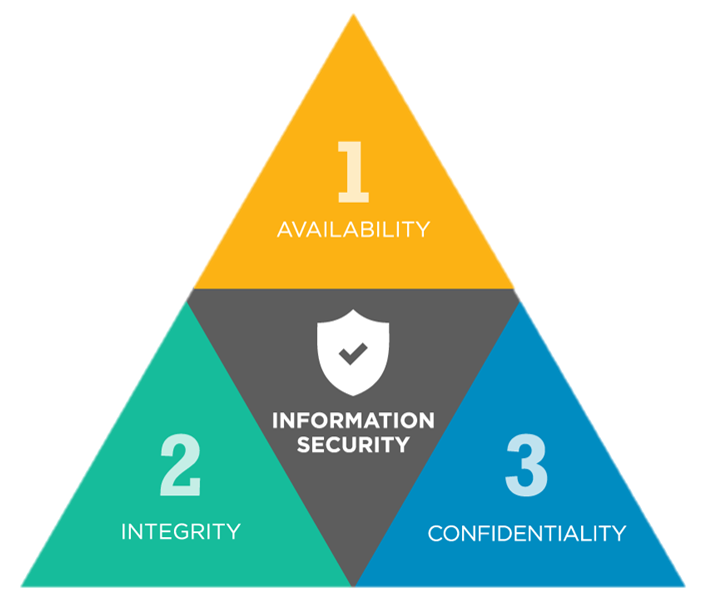
\includegraphics[width=0.5\textwidth]{images/CIA-graph.png}
    \caption{Principles of information security}
    \label{fig:cia-graph}
\end{figure}

\paragraph{Confidentiality} 
Confidentiality ensures that sensitive information is only accessible to authorized users. Techniques such as encryption, user authentication, and access control policies prevent unauthorized data access. While DoS attacks do not typically aim to breach confidentiality directly, successful exploitation may lead to indirect confidentiality violations if attackers cause service misconfigurations or force failovers to insecure states.

\paragraph{Integrity} 
Integrity guarantees that data is accurate and unaltered. It is maintained through cryptographic hash functions, checksums, and digital signatures that validate whether data has been tampered with. During a DoS attack, integrity may be compromised by interrupting legitimate updates or corrupting processes due to system overload.

\paragraph{Availability} 
Availability ensures that services and systems remain accessible to legitimate users at all times. This principle is the primary target of DoS attacks, which flood networks or services with excessive requests, causing slowdowns or complete denial of access. Maintaining availability involves redundancy, load balancing, and proactive mitigation strategies like rate limiting and firewalls.

\subsubsection{Extended Security Principles}
\paragraph{Non-repudiation} 
Non-repudiation guarantees that an entity cannot deny having performed a particular action, such as sending a message or initiating a transaction. This is enforced through digital signatures and secure logging mechanisms. In the context of DoS attacks, non-repudiation helps trace attack origins and supports legal accountability.

\paragraph{Authenticity} 
Authenticity confirms that data, communications, or users are genuine and not forged. Authentication protocols, digital certificates, and cryptographic techniques are used to ensure that data comes from trusted sources. This is crucial for filtering legitimate traffic from spoofed attack traffic in DoS scenarios.

\paragraph{Accountability} 
Accountability ensures that all actions within a system can be traced to responsible users or processes. It involves logging, auditing, and monitoring to track behavior. Accountability is vital for forensic analysis after a DoS attack and for strengthening defenses against future intrusions.

\section{Denial-of-Service (DoS) Attacks}
\paragraph{Introduction} 
Denial-of-Service (DoS) attacks aim to make a system or network resource unavailable to its intended users by overwhelming it with excessive traffic or exploiting protocol-level vulnerabilities. These attacks can disrupt services, degrade performance, or completely shut down access. The most common types include:

\begin{figure}[ht]
    \centering
    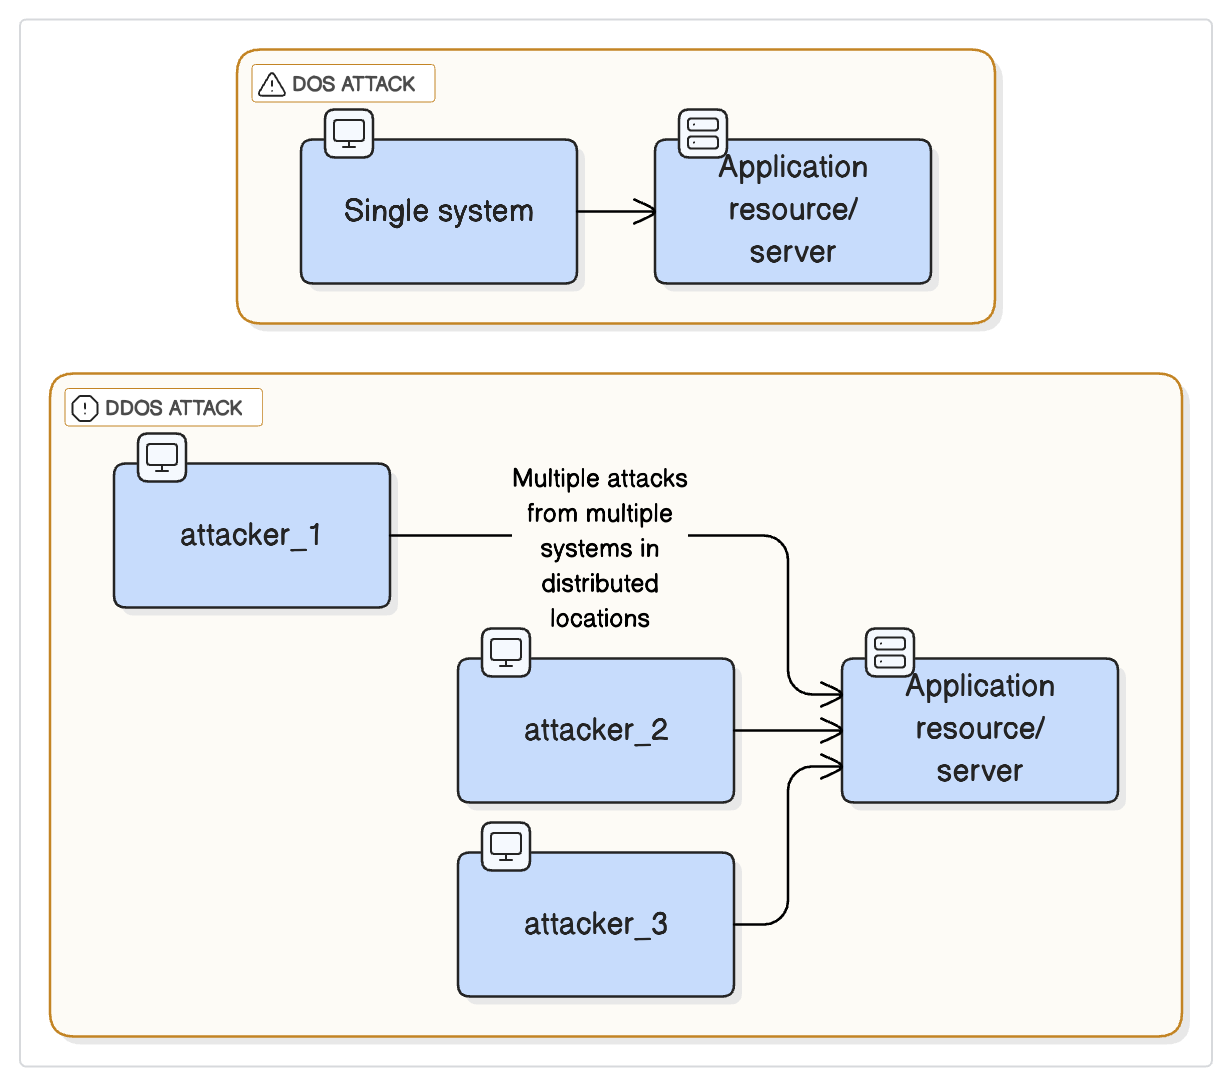
\includegraphics[width=0.8\textwidth]{images/dos-ddos-graph.png}
    \caption{DoS and DDoS Attack Traffic Comparison}
    \label{fig:dos-ddos-graph}
    \vspace{-0.5em}
\end{figure}

\subsection{Volumetric Attacks}
Volumetric attacks aim to saturate a target’s bandwidth by generating an overwhelming amount of traffic. This often involves amplification techniques or high-rate packet floods. Common examples include UDP floods and DNS amplification attacks, which leverage misconfigured servers to multiply traffic directed at the victim~\cite{fidelis_dos}.

In a UDP flood, attackers send large numbers of spoofed UDP packets to random or specific ports, consuming bandwidth and processing power. DNS amplification uses small queries to open resolvers with the victim’s IP address, causing them to return large responses to the victim. 

A notable example is the Mirai botnet, which infected hundreds of thousands of insecure IoT devices to coordinate massive traffic streams toward its targets~\cite{fidelis_dos}. The goal of volumetric attacks is to clog network links (Gbps or Tbps scale), preventing legitimate access.

\subsection{Protocol Attacks}
Protocol attacks exploit weaknesses in Layer 3/4 protocols (network or transport layer) to exhaust server or network resources. Unlike volumetric attacks, they do not require high bandwidth but instead consume stateful resources like connection tables or CPU cycles~\cite{fidelis_dos}.

A classic example is the TCP SYN flood, where attackers send numerous SYN packets without completing the handshake, filling the server’s connection queue~\cite{imperva_dos}. ICMP floods and Ping of Death attacks exploit the Internet Control Message Protocol to crash or freeze systems by sending malformed or excessive traffic.

Other examples include fragmentation attacks (e.g., Teardrop), which send overlapping IP fragments to crash reassembly logic, and ACK/FIN floods that exhaust firewall state tables.

\subsection{Application Layer Attacks}
Application-layer (Layer 7) attacks generate traffic that appears legitimate at the application level but consumes excessive server resources such as CPU, memory, or threads~\cite{fidelis_dos}. These attacks are difficult to detect because they mimic real user behavior.

HTTP GET/POST floods can overwhelm web servers by triggering costly operations. A well-known example is Slowloris, which sends partial HTTP headers slowly to hold open many connections and exhaust the web server’s pool~\cite{netscout_slowloris}. Other examples include RUDY (R-U-Dead-Yet) attacks and HTTP floods targeting dynamic or database-backed content.

\subsection{Distributed Denial-of-Service (DDoS)}
DDoS attacks use multiple compromised machines (botnets) to launch coordinated attacks, making them harder to block and vastly more powerful than single-source DoS attacks~\cite{fidelis_dos}.

Botnets like Mirai leverage IoT devices to simultaneously launch volumetric or protocol-based attacks. Reflective amplification (e.g., using open DNS/NTP servers) further increases traffic impact. Mitigation requires upstream filtering, rate-limiting, and often third-party scrubbing services.

\subsection{Network Traffic Analysis}
Mitigating DoS/DDoS attacks relies on monitoring and anomaly detection. This involves establishing a baseline of normal network behavior and identifying deviations in volume, protocol use, or source IPs~\cite{fidelis_dos, mdpi_dos}.

Anomaly-based intrusion detection systems (IDS) can flag unusual spikes, connection patterns, or TCP flag anomalies. Signature-based systems match known attack patterns. Flow analysis tools (e.g., NetFlow, sFlow) help detect irregular byte/packet rates or unusual source-destination pairs.

Advanced methods include machine learning to classify deviations. Once detected, defenses such as rate limiting, traffic shaping, or redirection to mitigation services are employed to maintain availability.

\section{Intrusion Detection Systems (IDS)}
An \textbf{Intrusion Detection System (IDS)} is a cybersecurity solution designed to monitor network or system activities for malicious actions or policy violations. Upon detecting such activities, the IDS typically alerts system administrators or integrates with centralized security tools like Security Information and Event Management (SIEM) systems to facilitate a coordinated response \cite{ibm_ids}.

\subsection{IDS Architecture}
\begin{figure}[H]
    \centering
    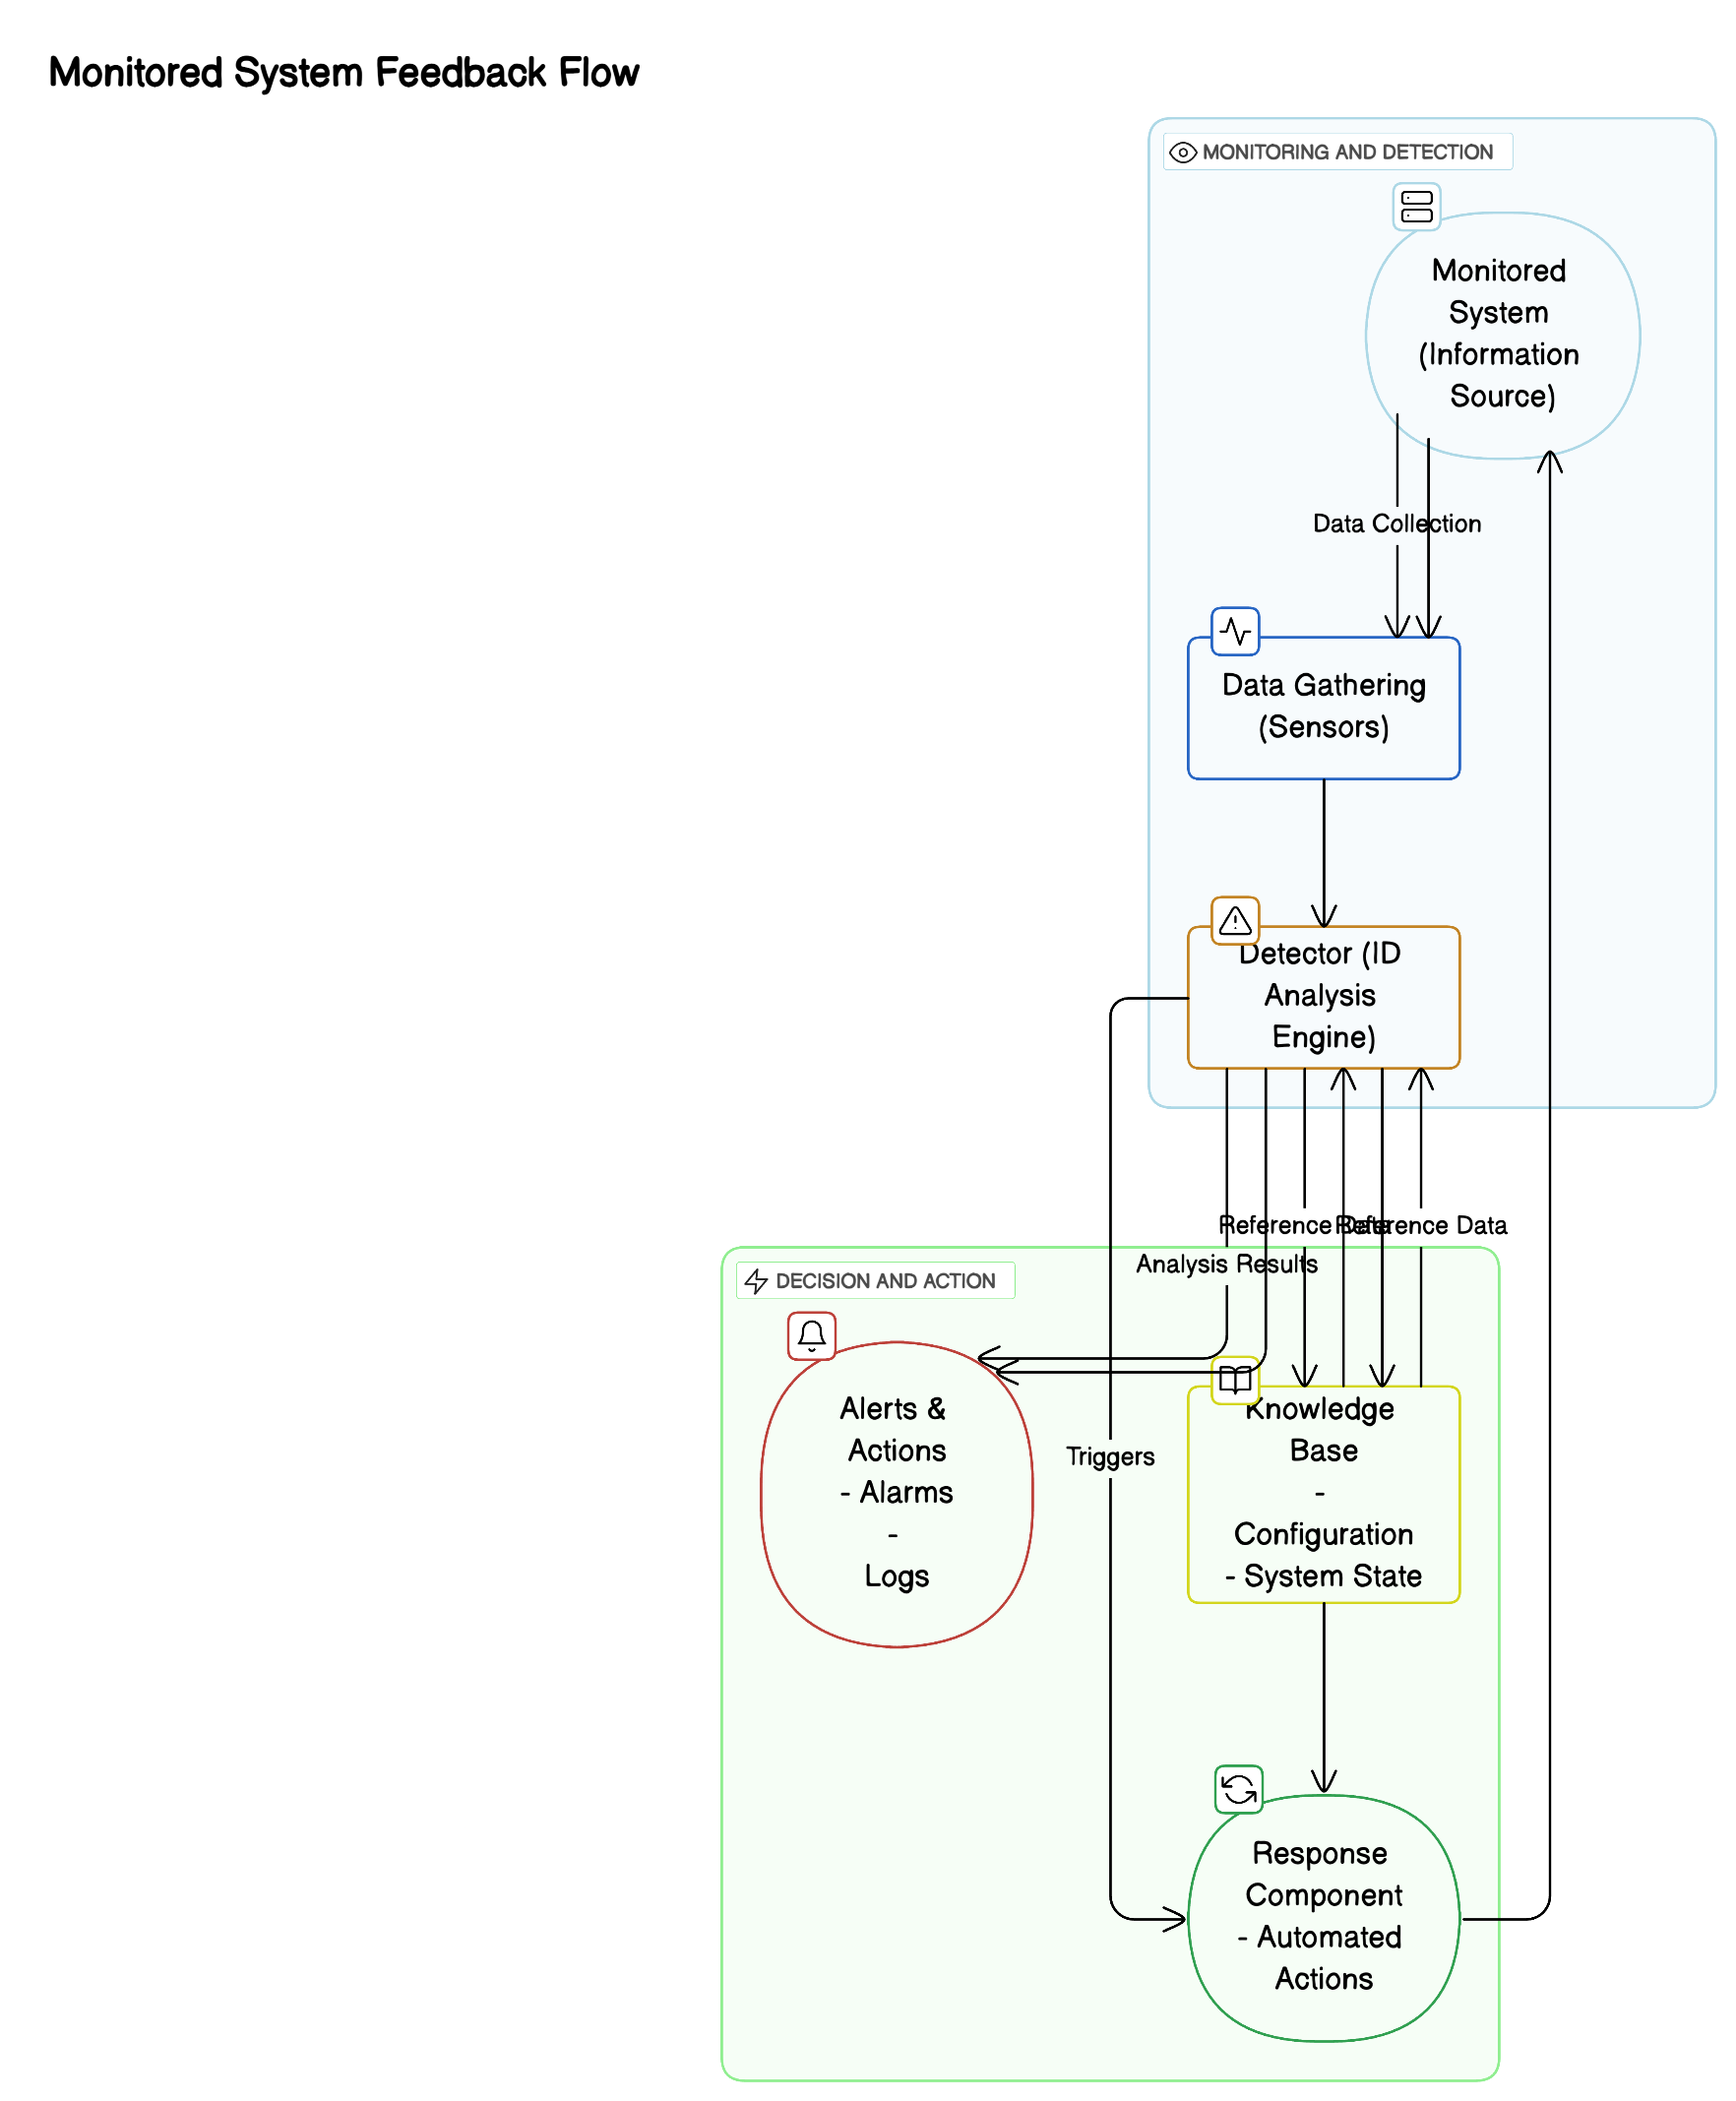
\includegraphics[width=0.8\textwidth]{images/ids-arch-diagram.png}
    \caption{Network-based Intrusion Detection System (NIDS) Architecture}
    \label{fig:nids-architecture}
\end{figure}

Modern IDS platforms implement modular architectures with several key components:
\begin{itemize}
    \item \textbf{Sensors:} are the front line of an IDS, deployed at strategic network chokepoints—such as mirror (SPAN) ports, network taps, or virtual interfaces in cloud environments—to collect raw traffic data.
    \item \textbf{Analysis Engines:} form the IDS's "brain," taking the sensor-collected data and applying a mixture of rule-based and intelligent techniques to detect threats.
    \item \textbf{Knowledge Base:} underpins all detection logic by maintaining up-to-date signatures, behavioral profiles, and historical datasets.
    \item \textbf{Response Systems:} close the loop between detection and defense. Once the analysis engine assigns a confidence score to an event, the response component generates alerts.
\end{itemize}
For DOS attack detection, these components must operate with high efficiency and scale to process enormous traffic volumes during attack scenarios.

\subsection{IDS Types and Functionality}
Intrusion Detection Systems serve as the primary monitoring and detection layer for network security threats, including DOS attacks:
\begin{itemize}
    \item \textbf{Network-based IDS (NIDS):} A NIDS is a monitoring solution placed at key junctions within a network to passively capture and inspect all passing traffic.
        \begin{figure}[ht]
            \centering
            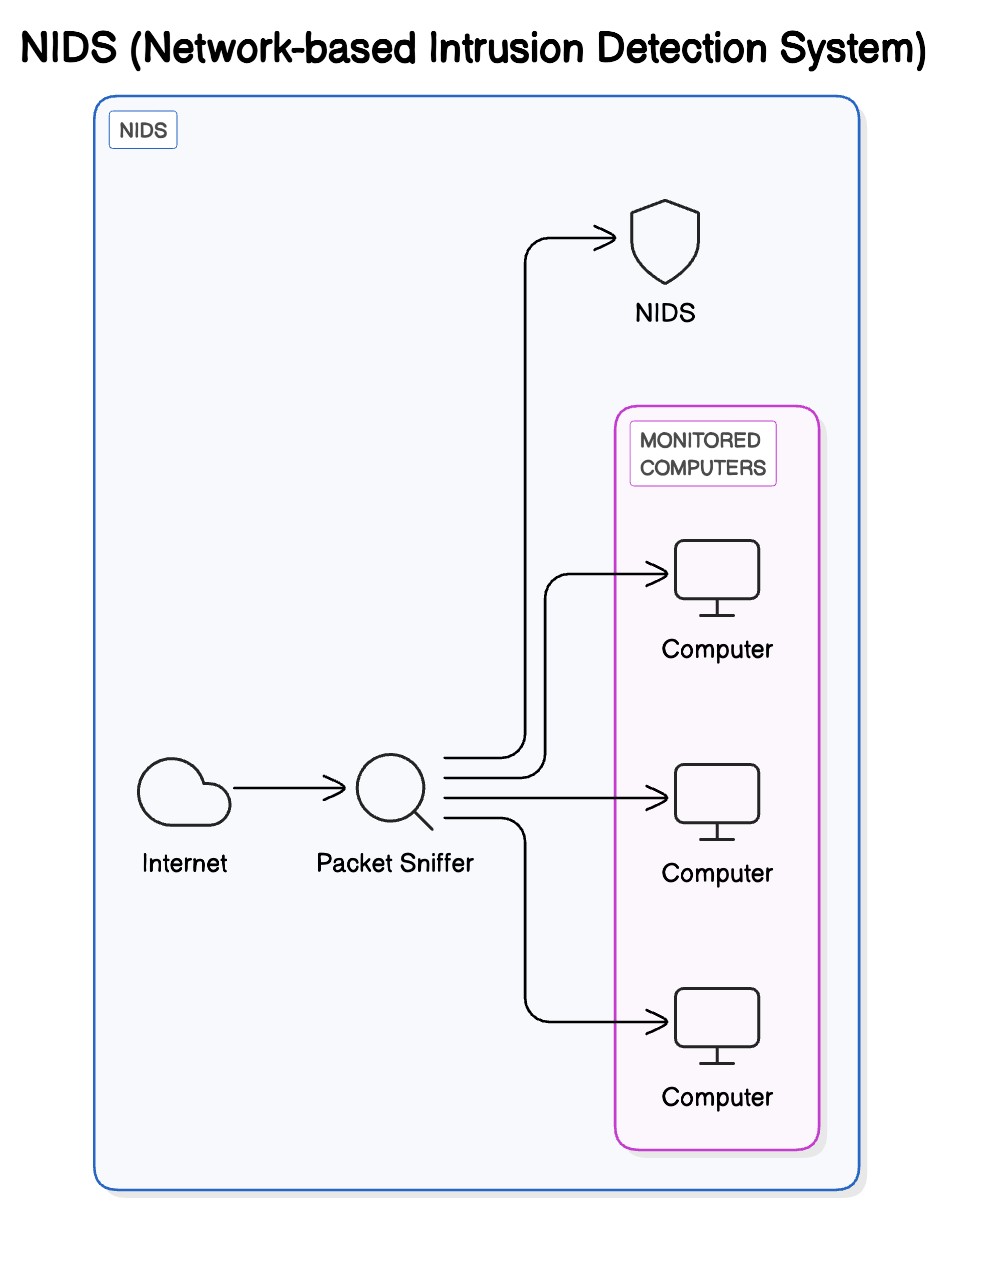
\includegraphics[width=0.8\textwidth]{images/nids-diagram.png}
            \caption{Network-based Intrusion Detection System (NIDS) Diagram}
            \label{fig:nids-diagram}
        \end{figure}
    \item \textbf{Host-based IDS (HIDS):} A HIDS operates at the level of individual endpoints or servers, offering deep visibility into system-specific activities.
        \begin{figure}[ht]
            \centering
            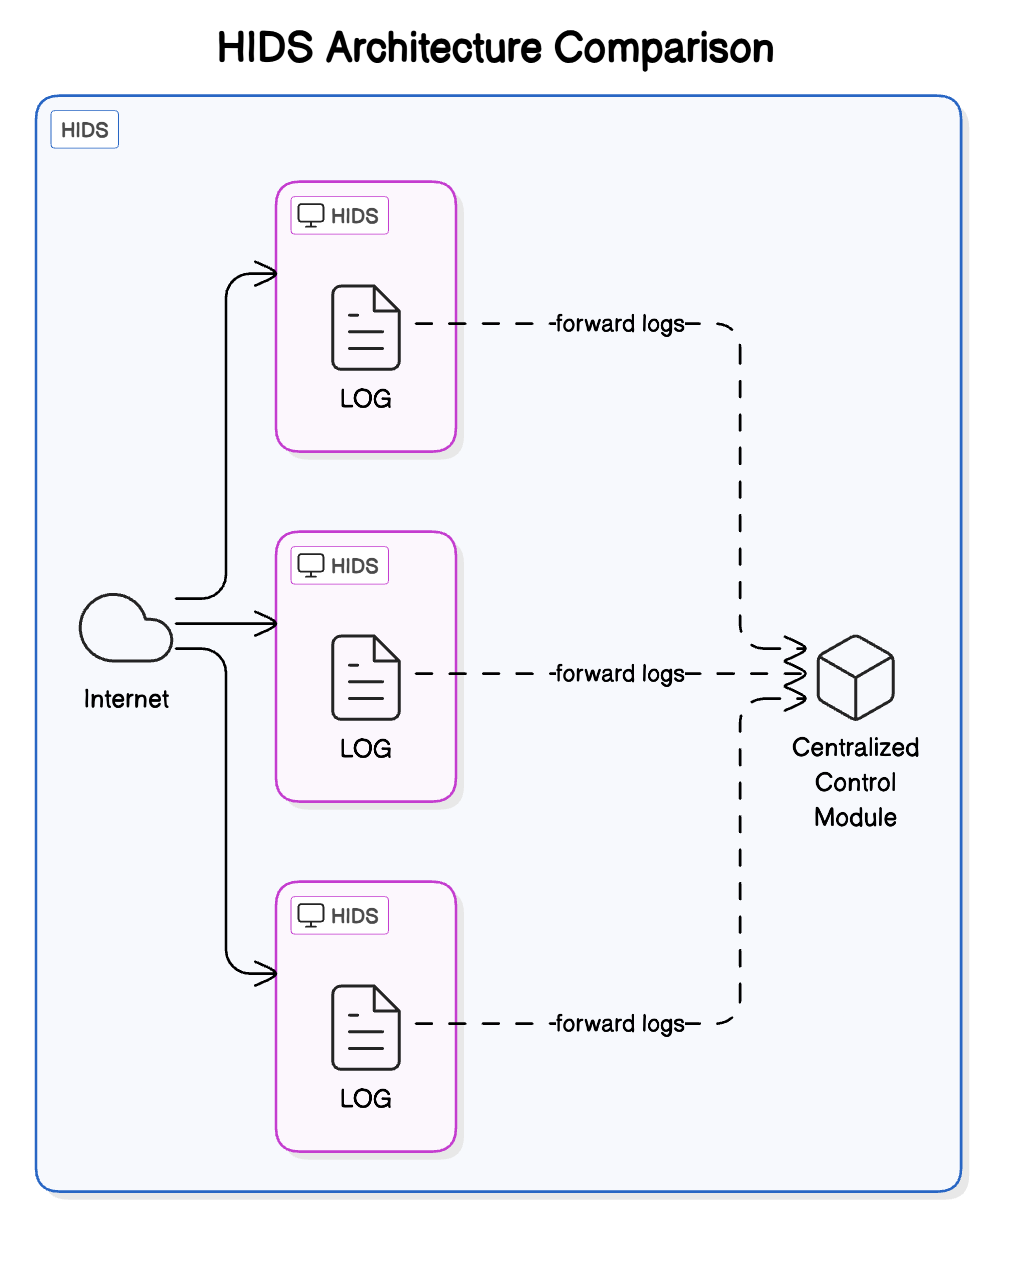
\includegraphics[width=0.8\textwidth]{images/hids-diagram.png}
            \caption{Host-based Intrusion Detection System (HIDS) Diagram}
            \label{fig:hids-diagram}
        \end{figure}
    \item \textbf{Detection Methodologies:}
    \begin{itemize}
        \item \textbf{Signature-based:} Matches observed traffic against known attack patterns (signatures). Highly effective for known attacks but ineffective against zero-day attacks.
        \item \textbf{Anomaly-based:} Establishes baselines of normal behavior and flags significant deviations. Can detect unknown attacks but may generate more false positives.
        \item \textbf{Hybrid Systems:} Combine both methodologies to leverage their respective strengths and reduce false positives.
    \end{itemize}
\end{itemize}

Limitations of Traditional IDS for DOS attack detection include difficulty processing high-volume traffic, distinguishing flash crowds from attacks, limited adaptation, high false-positive rates, and high resource consumption. These limitations necessitate AI-driven approaches like reinforcement learning.

\section{Classification in Security Contexts}
\subsection{Classification Paradigms}
Classification forms the foundation of automated threat detection:
\textbf{Binary Classification:} Distinguishes between normal and attack traffic.
\textbf{Multi-class Classification:} Distinguishes between multiple attack types.
\textbf{Hierarchical Classification:} Structures threats in a tree-like format.
\textbf{Multi-label Classification:} Assigns multiple categories to a single traffic flow.

\section*{What is Machine Learning?}
Machine learning (ML) is a branch of artificial intelligence (AI) focused on enabling computers and machines to imitate the way that humans learn. The learning system consists of a decision process, an error function, and a model optimization process.

\subsection{Machine Learning Techniques}
\section*{Supervised Learning}
Supervised learning involves training on labeled datasets. Common algorithms include Random Forests, Support Vector Machines (SVM), and Neural Networks.

\section*{Unsupervised Learning}
Unsupervised learning focuses on uncovering patterns in unlabeled data. Techniques include clustering (k-means) and anomaly detection (Isolation Forest).

\section*{Semi-Supervised Learning}

\chapter{Deep Q-Learning for Intrusion Detection}
\label{chap:dqn-for-ids}

\section{Introduction}
This chapter establishes the theoretical foundation for the novel intrusion detection methodology proposed in this thesis. The objective is to move beyond traditional, static detection systems by leveraging the adaptive and autonomous capabilities of modern artificial intelligence. We begin by introducing the key concepts of Deep Learning (DL), which provides the powerful function approximation tools needed to handle complex, high-dimensional data.

Subsequently, we delve into the paradigm of Reinforcement Learning (RL), a field of machine learning focused on goal-oriented learning through interaction. We will outline the fundamental components of an RL system—the agent, environment, states, actions, and rewards—that form the basis of sequential decision-making.

The core of this chapter brings these two fields together in the form of Deep Q-Learning (DQN). We will explain how DQN combines the perceptive power of deep neural networks with the decision-making framework of Q-learning to solve complex problems with large state spaces. Finally, we discuss the application of these advanced techniques to the domain of Intrusion Detection Systems (IDS), setting the stage for the specific architectural designs and experiments detailed in the subsequent chapters.

\section{Deep Learning: Key Concepts}
Deep Learning (DL) is a subfield of machine learning inspired by the structure and function of the human brain, utilizing artificial neural networks with multiple layers—hence the term "deep." Unlike traditional machine learning models that often rely on manually engineered features, deep learning models are designed to learn hierarchical representations of data automatically. By processing data through successive layers, they can identify simple patterns at the initial layers and compose them into more complex and abstract patterns at deeper layers. This makes them exceptionally powerful for finding intricate structures in large, high-dimensional datasets, such as those found in network traffic analysis.

\begin{figure}[H]
    \centering
    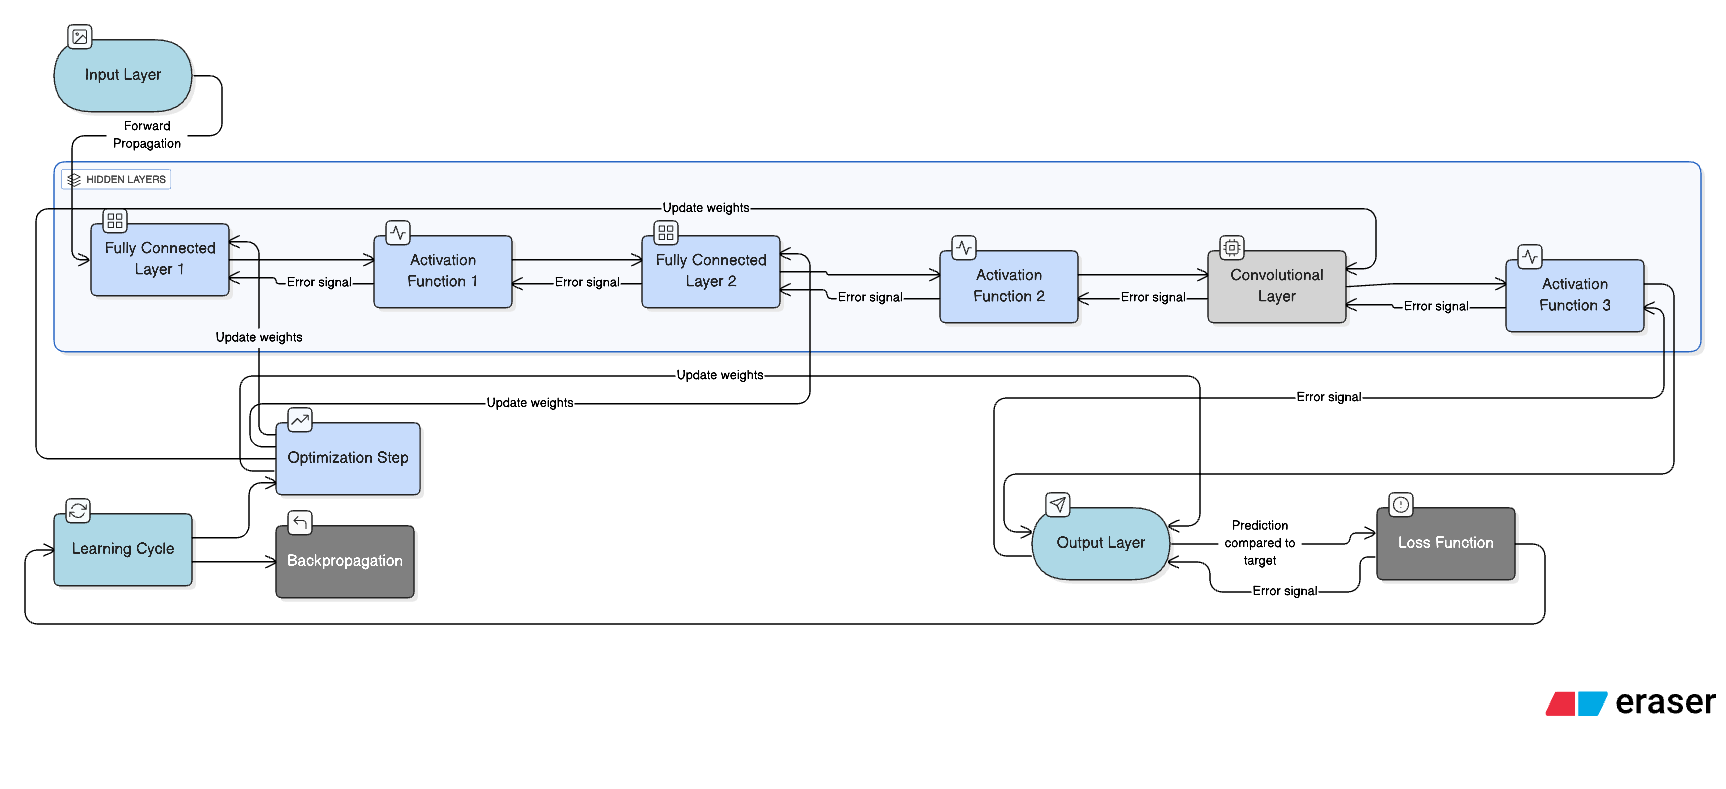
\includegraphics[width=0.8\textwidth]{images/deep-learning-graph.png}
    \caption{Fundamental structure of a deep neural network, showing the flow from input data through hidden layers to an output prediction.}
    \label{fig:deep-learning-graph}
\end{figure}

A typical neural network, as illustrated in Figure \ref{fig:deep-learning-graph}, consists of an input layer, one or more hidden layers, and an output layer. Each layer contains interconnected nodes known as \textbf{neurons}. A neuron computes a weighted sum of its inputs, adds a bias term, and then passes this result through a non-linear \textbf{activation function}. The purpose of the activation function (e.g., ReLU, Sigmoid, Tanh) is crucial: it introduces non-linearity into the model, enabling the network to learn complex relationships that a purely linear model could not capture. The connections between neurons have associated \textbf{weights} and \textbf{biases}, which are the learnable parameters that the network adjusts during training to minimize its prediction error.

The process of training a deep neural network is an iterative optimization cycle aimed at finding the optimal set of weights and biases. This cycle generally involves the following steps:
\begin{enumerate}
    \item \textbf{Forward Propagation:} Input data (e.g., a feature vector from a network flow) is fed into the network's input layer. The data then propagates forward through the hidden layers. At each layer, every neuron performs its computation, and its output becomes the input for the next layer. This process continues until a final prediction is generated at the output layer. This step is essentially the network making its "best guess" based on its current parameters.

    \item \textbf{Loss Function:} The network's prediction is compared to the true value (the ground-truth label) using a \textbf{loss function}. The loss function quantifies the discrepancy or error between the prediction and the actual target. For classification tasks like ours, the \textbf{Cross-Entropy loss} is commonly used. A high loss value indicates a poor prediction, while a low loss value signifies a good one. The goal of training is to minimize this loss.

    \item \textbf{Backpropagation:} This is the core mechanism for learning. Based on the calculated loss, the error is propagated backward through the network, from the output layer to the input layer. Using the chain rule from calculus, backpropagation efficiently calculates the gradient of the loss function with respect to each weight and bias in the network. This gradient essentially represents the contribution of each parameter to the total error—it tells the network "in which direction" and "by how much" each weight should be adjusted to reduce the error.

    \item \textbf{Optimization:} An \textbf{optimization algorithm}, such as Adam or Stochastic Gradient Descent (SGD), uses the gradients computed during backpropagation to update the network's weights and biases. It adjusts the parameters in the opposite direction of their gradient, effectively taking a small step towards a lower loss. The size of this step is controlled by a hyperparameter called the \textbf{learning rate}.
\end{enumerate}
This cycle of forward propagation, loss calculation, backpropagation, and optimization is repeated for many iterations (or "epochs") over the training dataset. With each iteration, the network's parameters are fine-tuned, and it gradually becomes better at making accurate predictions, converging towards a state of minimal error.

In this thesis, we utilize two primary deep learning architectures to serve as the Q-network for our agent:

\paragraph{Multi-Layer Perceptron (MLP)} The MLP is the quintessential deep learning model. It consists of one or more fully connected hidden layers, where every neuron in a given layer is connected to every neuron in the subsequent layer. It is a universal function approximator, well-suited for processing structured, tabular data where the input is a flat vector of features and there is no inherent spatial or temporal relationship between them.

\paragraph{Convolutional Neural Network (CNN)} Originally designed for image processing, CNNs excel at detecting spatial hierarchies and patterns in grid-like data. They use specialized layers with filters (or kernels) that slide across the input, detecting local patterns such as edges or textures. By stacking these layers, a CNN can learn to recognize increasingly complex features. As we will detail later, we adapt this powerful architecture to our tabular network data by reshaping the 1D feature vector into a 2D "feature-image," allowing the CNN to discover localized correlations between related network features.
\section{Reinforcement Learning}
Reinforcement Learning (RL) is a paradigm of machine learning where an autonomous \textbf{agent} learns to make optimal decisions by interacting with an \textbf{environment}. Unlike supervised learning, the agent is not given explicit correct answers. Instead, it receives feedback in the form of numerical \textbf{rewards} or penalties for its actions, and its goal is to learn a strategy, or \textbf{policy}, that maximizes its cumulative reward over time.

The core components of the RL framework are (see Figure \ref{fig:rl-diagram}):
\begin{itemize}
    \item \textbf{Agent:} The learner and decision-maker. In our context, this is the intrusion detection model.
    \item \textbf{Environment:} The external world with which the agent interacts. For our task, this is the network traffic environment.
    \item \textbf{State ($s_t$):} A snapshot of the environment at a specific time step $t$. This could be a vector of features describing a network flow.
    \item \textbf{Action ($a_t$):} A choice made by the agent in a given state. For example, classifying the traffic as 'Benign' or 'Attack'.
    \item \textbf{Reward ($r_t$):} A scalar feedback signal the agent receives after taking an action. A positive reward encourages the action, while a negative reward (penalty) discourages it.
\end{itemize}

\begin{figure}[H]
    \centering
    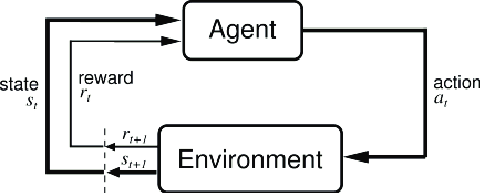
\includegraphics[width=0.8\textwidth]{images/rl-diagram.png}
    \caption{The Agent-Environment Interaction Loop in Reinforcement Learning}
    \label{fig:rl-diagram}
\end{figure}

The agent's goal is to learn a policy $\pi(a|s)$ that maps states to actions in a way that maximizes the expected cumulative discounted reward, known as the \textit{return}. A fundamental challenge in RL is the \textbf{exploration-exploitation trade-off}: the agent must exploit its current knowledge to get high rewards but also explore new, untried actions to discover potentially better strategies.

To guide its decisions, the agent learns a \textbf{value function}. A key type is the action-value function, or \textbf{Q-function}, denoted as $Q(s, a)$. This function estimates the expected return of taking action $a$ in state $s$ and then following the policy thereafter. The optimal Q-function, $Q^*(s, a)$, provides the maximum possible return, and an agent that knows this function can act optimally by simply choosing the action with the highest Q-value in any given state.

\section{Deep Q-Learning (DQN)}
Traditional Q-learning algorithms use a table (a "Q-table") to store the Q-value for every possible state-action pair. This approach becomes completely infeasible for problems with large or continuous state spaces, such as those encountered in network traffic analysis, where the number of possible states is virtually infinite.

\textbf{Deep Q-Learning (DQN)} overcomes this limitation by merging deep learning with Q-learning. Instead of a Q-table, DQN uses a deep neural network as a function approximator to estimate the Q-function, $Q(s, a; \theta)$, where $\theta$ represents the network's weights. The network takes a state $s$ as input and outputs a Q-value for each possible action.

To ensure stable learning, the original DQN algorithm introduced two key innovations:
\begin{enumerate}
    \item \textbf{Experience Replay:} The agent stores its experiences—tuples of $(s_t, a_t, r_t, s_{t+1})$—in a large memory buffer. During training, it samples random mini-batches of experiences from this buffer to update the Q-network. This technique breaks the temporal correlations between consecutive samples, leading to more stable and efficient learning.
    \item \textbf{Target Network:} DQN uses a second, separate neural network called the target network. This network is a periodically updated copy of the main (online) Q-network. It is used to generate stable "target" Q-values for the learning updates. The loss is calculated as the difference between the Q-value predicted by the online network and the target value calculated using the Bellman equation with the target network:
\end{enumerate}

The target Q-value, $y_t$, is computed as:
\begin{equation}
y_t = r_t + \gamma \max_{a'} Q(s_{t+1}, a'; \theta^-)
\end{equation}
Here, $\gamma$ is the discount factor that balances immediate and future rewards, $\theta$ represents the parameters of the online network, and $\theta^-$ represents the parameters of the fixed target network. The network is then trained by minimizing a loss function (e.g., Mean Squared Error) between its prediction $Q(s_t, a_t; \theta)$ and the target $y_t$.
 Deep Q-Learning is a powerful extension of the traditional Q-Learning algorithm that leverages deep neural networks to approximate the Q-value function. In standard Q-Learning, an agent maintains a Q-table that maps state-action pairs to expected future rewards. However, this becomes impractical for environments with large or continuous state spaces. Deep Q-Learning addresses this limitation by using a deep neural network, known as a Q-network, to estimate Q-values directly from raw input states.

In reinforcement learning, the agent interacts with the environment in discrete time steps. At each step $t$, the agent observes a state $s_t$, selects an action $a_t$, receives a reward $r_t$, and transitions to a new state $s_{t+1}$. The goal is to learn a policy $\pi$ that maximizes the expected cumulative reward over time.

The Q-value function $Q(s, a)$ represents the expected return of taking action $a$ in state $s$ and following the policy thereafter. In Deep Q-Learning, the Q-network is trained to minimize the difference between the predicted Q-value and the target Q-value, which is computed using the Bellman equation:

\begin{equation}
Q(s\_t, a\_t) = r\_t + \gamma \max\_{a'} Q(s\_{t+1}, a'; \theta^-)
\end{equation}

Here, $\gamma$ is the discount factor, $\theta$ are the parameters of the current Q-network, and $\theta^-$ are the parameters of a target network that is periodically updated to stabilize training.

To improve learning stability and efficiency, Deep Q-Learning introduces two key techniques:
\begin{itemize}
\item \textbf{Experience Replay:} Stores past experiences in a replay buffer and samples mini-batches randomly during training to break correlations between consecutive samples.
\item \textbf{Target Network:} Uses a separate, periodically updated target network to compute the target Q-values, reducing oscillations and divergence.
\end{itemize}

Deep Q-Learning has been successfully applied to various complex decision-making tasks, such as playing Atari games directly from raw pixels, demonstrating its potential in handling high-dimensional input spaces.


%  \begin{center}
%     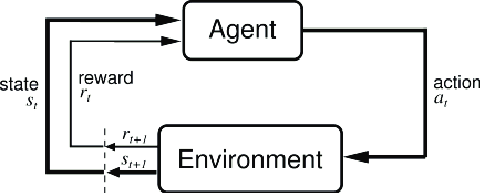
\includegraphics[width=0.8\textwidth]{images/rl-diagram.png} \\
%     \textit{Figure: Basic Components of Reinforcement Learning}
%   \end{center}

\section{Environment Modeling for DoS Detection}

The foundation of any RL application is a well-designed environment that accurately represents the problem domain. For DoS detection, this environment must model network traffic patterns and attack scenarios in a way that enables effective learning.

\subsection{State Space Design}

The state space in a reinforcement learning (RL) framework for Denial-of-Service (DoS) detection encodes the essential characteristics of network traffic that the agent uses to make decisions. A well-designed state space should reflect a comprehensive yet efficient representation of the network environment, enabling the RL agent to distinguish between normal and malicious activity. This design typically integrates four categories of features: traffic volume metrics, statistical distribution properties, temporal behavior indicators, and content-based descriptors. Each category offers a unique perspective on the nature of the traffic, contributing to a robust and informative state representation.

Traffic volume features quantify the scale and frequency of network activity. These include metrics such as packets per second, bytes per second, flow initiation rates, and the number of concurrent connections. These indicators are particularly useful for detecting volumetric DoS attacks, which are characterized by sudden spikes in traffic volume designed to overwhelm network resources. By monitoring these patterns, the RL agent can quickly recognize and react to abnormal surges in activity.

Statistical distribution features capture how traffic attributes are spread across various dimensions. Entropy values of source and destination IP addresses, protocol usage percentages, port distributions, and packet size variation are key indicators in this category. These features help identify anomalies that are not necessarily reflected in overall traffic volume but manifest as irregularities in distribution patterns, such as a high concentration of traffic targeting a specific port or originating from a narrow set of addresses.

Temporal pattern features provide insight into the evolution of traffic over time. By analyzing short-term trends, comparing current behavior to historical baselines, or evaluating periodicity, the agent can detect subtle or persistent attack patterns. Features such as time-of-day normalization or trend analysis allow the RL agent to differentiate between expected daily fluctuations and genuinely suspicious behavior, such as traffic bursts that align with known attack schedules.

Content-based features delve into the specifics of packet content and header information. This includes identifying protocol anomalies, unusual header field values, payload characteristics (when available), and application-layer request patterns. Such features are crucial for detecting more sophisticated attacks that may not exhibit volume or distribution anomalies but instead exploit specific protocol vulnerabilities or payload structures.

A critical aspect of state space design is balancing informativeness with efficiency. High-dimensional state representations can slow down learning and lead to overfitting. To mitigate this, techniques like feature selection, dimensionality reduction, and hierarchical representations can be employed. These methods help retain the most relevant features while reducing computational overhead, ultimately enhancing the agent’s learning performance and scalability.

\subsection{Action Space Definition}

The action space defines the set of all possible decisions or interventions that the reinforcement learning (RL) agent can make in response to observed network conditions. In the context of DoS detection systems, these actions are typically organized into three main categories: detection-related, response-related, and adaptive actions. Each category serves a distinct role in enabling the agent to not only identify malicious activity but also to react appropriately and adjust its behavior over time.

Detection-related actions allow the agent to classify the nature of incoming traffic. These may include flagging traffic as normal, marking it as a potential DoS attack with low confidence, confirming it as a high-confidence DoS event, or requesting additional inspection to reduce uncertainty. These actions contribute to the agent’s ability to differentiate between benign and malicious behavior with varying degrees of certainty.

Response-related actions are used to enforce protective measures against suspicious or confirmed attack traffic. These actions include allowing traffic to proceed unimpeded, rate-limiting suspected malicious flows, blocking specific traffic patterns known to be harmful, or redirecting traffic for more detailed analysis by external systems. Such actions form the core of the system's active defense mechanism, enabling real-time mitigation of ongoing threats.

Adaptive actions provide the agent with the ability to adjust its operational parameters in response to evolving threat landscapes. This includes actions such as modifying monitoring sensitivity, tuning feature extraction processes, escalating suspicious cases to human analysts, or gathering additional contextual data to refine future decision-making. These adaptive strategies are essential for maintaining long-term performance in dynamic environments.

The granularity of the action space plays a critical role in determining both the learning efficiency and the practical utility of the RL system. An overly coarse action space may restrict the agent's responsiveness and lead to underfitting, whereas an excessively fine-grained space can increase the complexity of the learning problem and slow convergence. Therefore, careful design of the action space is essential to strike an optimal balance between expressiveness and tractability.


\subsection{Reward Function Design}

The reward function plays a pivotal role in shaping the learning behavior of the reinforcement learning (RL) agent, guiding it toward effective and efficient DoS detection strategies. A well-crafted reward function must strike a balance between multiple, often competing objectives such as detection accuracy, operational efficiency, and timely response.

In terms of detection accuracy, the agent is incentivized through positive rewards for correctly identifying attacks, while being penalized for false positives and false negatives. These penalties and rewards may be further weighted based on the severity of the detected attack and the agent’s confidence in its classification. This ensures that the agent not only learns to detect attacks but also to assess their impact and act accordingly.

Operational efficiency is also integral to the reward function. Small penalties may be applied to account for resource consumption, including computational overhead and bandwidth usage. Additionally, time-based rewards can encourage early detection, while excessive inspection of normal traffic or inefficient use of mitigation mechanisms can incur penalties. These components help align the agent’s behavior with real-world constraints and performance expectations.

A typical structure for the reward function may take the following form:

\begin{equation}
R(s, a, s') = w_{1} \times \text{DetectionAccuracy} + w_{2} \times \text{TimeToDetect} + w_{3} \times \text{ResourceEfficiency}
\end{equation}

In this formulation, \textit{DetectionAccuracy} reflects the correctness of the classification, considering true positives, false positives, and false negatives. \textit{TimeToDetect} quantifies the latency in identifying an attack, and \textit{ResourceEfficiency} evaluates how judiciously the system utilizes its resources during detection and response. The weights \(w_{1}, w_{2}, w_{3}\) are tunable parameters that allow the system to prioritize objectives based on organizational or operational goals.

Careful calibration of the reward function is essential to ensure that the agent develops policies that are not only accurate and robust but also practical within the resource constraints and real-time requirements of modern network environments.


\subsection{Environment Dynamics}

The environment dynamics define the mechanisms through which state transitions occur in response to the agent’s actions. In the context of DoS detection, these dynamics are influenced by both the underlying traffic patterns and the mitigation strategies employed by the agent. State transitions are often governed by probabilistic rules that reflect how network traffic evolves over time. For instance, specific traffic behaviors may be more or less likely to follow certain patterns, such as bursty traffic or sustained high-volume flows indicative of an ongoing attack.

The agent’s actions directly impact the state evolution. For example, blocking suspicious traffic may lead to a reduction in attack volume, altering the observable state characteristics. Similarly, redirecting traffic for analysis or applying rate limits can change flow distributions and entropy metrics within the network. It is also important to consider temporal aspects of the environment; the effects of certain actions may not be immediately visible. For instance, a rate-limiting policy might only manifest noticeable changes after a delay, as the network adapts or the attacker responds.

Modeling these dynamics accurately is essential for realistic simulation and effective training of reinforcement learning agents. It allows the agent to learn how its actions influence the environment and adjust its policy accordingly to achieve robust and adaptive DoS detection performance.



\subsection{Challenges in Applying RL to Security Domains}

While reinforcement learning (RL) holds significant potential for enhancing cybersecurity systems, its application to security contexts—particularly DoS detection—presents several unique challenges. One major hurdle is the high dimensionality of the state space. Network traffic generates vast and complex feature sets, requiring sophisticated representation and dimensionality reduction techniques to ensure tractable learning. 

Another difficulty lies in the delayed nature of rewards. In many cases, the outcome of a security-related decision—whether it successfully prevented an attack or caused unintended side effects—may only become clear after a considerable time delay. This complicates credit assignment and policy evaluation. Moreover, rewards in the security domain tend to be sparse; attack events are relatively rare in comparison to the continuous stream of benign network activity, making it difficult for the agent to gain useful feedback consistently.

Safety during the learning process is also a critical concern. Exploration, a core part of RL, must be managed carefully to avoid compromising system integrity. Unlike in traditional domains, erroneous actions in security systems can have severe consequences. Compounding this is the adversarial nature of the environment—attackers actively adapt their strategies to bypass detection mechanisms, forcing RL agents to learn in a moving target setting.

To address these challenges, structured educational frameworks and simulation environments can be employed. These offer controlled scenarios where RL techniques can be gradually introduced and refined before deployment in production systems.


\noindent\textbf{Source:} Adapted from GeeksforGeeks: What is Reinforcement Learning


Deep Q-Learning has been successfully applied to various complex decision-making tasks, such as playing Atari games directly from raw pixels, demonstrating its potential in handling high-dimensional input spaces.



\section{Conclusion}
This chapter has provided the essential theoretical background on Deep Learning, Reinforcement Learning, and their synthesis in Deep Q-Networks. We have established that the DQN framework, with its ability to handle high-dimensional data and learn optimal policies through interaction, is a powerful candidate for building a next-generation, adaptive Intrusion Detection System. By modeling the DoS detection task as an RL problem, we can leverage these advanced techniques to create a more intelligent and resilient defense mechanism. The following chapters will build upon this foundation to detail the specific implementation and empirical evaluation of our proposed DQN-based models.

\chapter{Designing DQN Architectures for DoS/DDoS Attack Detection}
\section{Introduction}

This chapter details the design and conceptualization of a robust Distributed Denial of Service (DDoS) attack detection system. We propose an innovative approach that leverages the power of Deep Q-Networks (DQN), a prominent algorithm in Reinforcement Learning (RL), by adapting it to the context of a supervised classification problem. The primary goal is to develop an intelligent agent capable of accurately identifying DoS/DDoS attacks in real-world network traffic scenarios.

The chapter begins by meticulously defining the problem within the RL framework, mapping traditional RL concepts such as states, actions, and rewards to the specifics of network intrusion detection. We then outline the comprehensive data preprocessing pipeline, which is crucial for preparing raw network traffic data for effective model training. Subsequently, we delve into the proposed Deep Q-Network (DQN) architectures, including discussions on the standard DQN and the enhanced Double DQN (DDQN), as well as integrating Convolutional Neural Networks (CNN) for advanced feature extraction. The operational mechanics of the DQN agent, encompassing the training loop and its core components, are thoroughly explained. This foundation lays the groundwork for the practical implementation and evaluation of these architectures in subsequent chapters.

% --- Preprocessing Pipeline Section ---
\section{Problem Modeling for DoS/DDoS Detection using DQN}

To leverage Reinforcement Learning (RL) for DDoS attack detection, we must reframe the classification task into an RL problem. This involves defining key RL components: the environment, rewards, agent's objective, and classification tasks within our context.

\subsection{Environment Definition}
In our framework, the "environment" is simulated by a preprocessed dataset. Each state (st​) is a single, preprocessed feature vector representing a snapshot of network traffic. Unlike traditional RL where states evolve from prior actions, here, the "next state" (st+1​) is functionally defined as the subsequent sample in a randomly shuffled batch. This approach allows us to estimate future value for Q-learning updates, even in a non-sequential data context. The dataset itself acts as the source of observations the agent makes at each "time step."

\subsubsection{Reward Function}

The reward ($r_t$) is an immediate scalar feedback signal provided by the simulated environment based on the agent's classification decision. It quantifies the quality of the agent’s chosen action ($a_t$) by directly comparing it with the known optimal action ($a_t^*$), i.e., the true label.

The reward function is defined as:

\[
r_t =
\begin{cases}
+10 & \text{if } a_t = a_t^* \quad \text{(Correct Classification)} \\
0   & \text{if } a_t \ne a_t^* \quad \text{(Incorrect Classification)}
\end{cases}
\]

Using a neutral reward of 0 for incorrect actions, rather than a negative penalty (e.g., $-1$), can lead to more stable training in some contexts, as it does not excessively punish the agent during its initial exploration phase. This reward mechanism forms the crucial bridge between the supervised ground-truth label and the reinforcement learning feedback loop.

\subsubsection{Agent's Objective}

The primary objective of the reinforcement learning (RL) agent is to learn an optimal detection policy $\pi(a \mid s)$ that maximizes its long-term cumulative reward. 

In the context of DDoS detection, this objective translates into maximizing the number of correct classifications—that is, accurately identifying both benign and malicious traffic. 

By continuously refining its understanding of the value associated with selecting a particular label in a given context, the agent aims to converge toward a strategy that minimizes misclassifications and ensures robust detection performance.

\subsubsection{Definition of Classification Tasks}

The problem is framed as a binary classification task to simplify the detection process. The agent's actions ($a_t$) correspond to the two possible classification labels:

\begin{itemize}
  \item \textbf{Action 0}: Classify the network traffic as \texttt{Benign}.
  \item \textbf{Action 1}: Classify the network traffic as \texttt{Attack} (encompassing any type of DoS/DDoS attack).
\end{itemize}

The multi-class labels present in the original dataset (e.g., \texttt{DrDoS\_NTP}, \texttt{SYN}, \texttt{UDP-lag}) are converted into this binary format during preprocessing. This transformation enables the model to focus on the fundamental task of distinguishing any malicious activity from normal network behavior.


\subsection{Data Preprocessing Pipeline}

The preprocessing phase is a fundamental component of building an effective machine learning model, ensuring that the input data is clean, consistent, and optimally formatted for the learning algorithm. Our approach involves several key steps:

\subsubsection{Dataset}

The primary dataset used for this research is a publicly available dataset. This dataset is highly relevant as it contains a variety of the most up-to-date common DDoS attacks alongside benign traffic, closely resembling real-world network scenarios. The data is provided in PCAP format and has been pre-processed using a specialized tool to generate labeled flows in CSV files. Each flow is characterized by features based on its time stamp, source and destination IPs, source and destination ports, and the protocol used.

\subsubsection{Step 1: Data Cleaning}
The initial phase focuses on cleaning the dataset to ensure its quality and integrity. This involves three key actions:

\begin{itemize}
    \item \textbf{Handling Null Values:} The dataset is first inspected for any missing or null values. Rows containing such values are dropped entirely. This step is crucial to prevent computational errors during model training and to ensure that the model learns from complete, high-quality samples.

    \item \textbf{Dropping Irrelevant Features:} Certain features that are unique to individual flows and do not contribute to generalizable attack patterns are removed. Including them would introduce noise and create a high risk of overfitting, where the model memorizes specific instances from the training data rather than learning the underlying behavior of attacks.

    \item \textbf{Numeric Conversion:} All remaining feature values are converted to a numeric data type. Machine learning models, and particularly neural networks like the DQN, require numerical input for their mathematical operations. This step ensures that all data, including any encoded categorical features, is in a format that the model can process.
\end{itemize}

\subsubsection{Step 2: Feature Selection using Random Forest Classifier}

Feature selection is a critical process for reducing the dimensionality of the dataset, which in turn reduces model complexity, decreases training time, and mitigates the risk of overfitting. For this task, we utilize the \textit{Random Forest Classifier}.

Random Forest is an ensemble learning method that constructs a multitude of decision trees during training. It provides a built-in measure of feature importance, which reflects the degree to which each feature contributes to improving the purity of the nodes in the trees. The process is as follows:

\begin{itemize}
    \item A Random Forest Classifier is trained on the cleaned dataset.
    
    \item The \texttt{feature\_importances\_} attribute of the trained model is used to extract an importance score for each feature.
    
    \item Features are ranked based on these scores, and only the top-ranked features that contribute most significantly to the model’s predictive power are retained for subsequent steps.
\end{itemize}

\subsubsection{Step 3: Data Normalization}


After feature selection, the data is normalized to ensure that all features contribute equally to the model’s learning process. We employ \textit{Min-Max normalization}, which scales each feature to a fixed range between 0 and 1.

This technique is essential for neural networks, as it prevents features with larger numeric ranges from dominating the learning process and helps stabilize the gradient descent optimization, leading to faster convergence.

The Min-Max normalization formula for a feature \( X \) is given by:

\[
X_{\text{normalized}} = \frac{X - X_{\min}}{X_{\max} - X_{\min}}
\]

where:

\begin{itemize}
    \item \( X_{\text{normalized}} \) is the scaled value,
    \item \( X \) is the original feature value,
    \item \( X_{\min} \) is the minimum value of the feature in the dataset,
    \item \( X_{\max} \) is the maximum value of the feature in the dataset.
\end{itemize}

\subsubsection{Step 4: Dataset Balancing with Random Undersampling}

The dataset exhibits a significant class imbalance, with a much larger proportion of attack traffic compared to benign traffic. Training a model on such an imbalanced dataset would bias it towards the majority class (attacks), leading to poor detection performance for the minority class (benign traffic) and a high false positive rate.

To address this, we apply \textit{random undersampling}. This technique balances the class distribution by reducing the number of samples from the majority class. Specifically, we randomly select and remove samples from the `attack` class until its size matches the number of samples in the `benign` class.

While this method risks discarding potentially useful information from the majority class, it is effective in creating a balanced dataset that enables the model to learn the distinguishing characteristics of both classes with equal importance. The result is a model that is more robust and accurate in classifying both attack and benign traffic.

\subsection{Proposed DQN Architectures for Attack Detection}

Having established the conceptual mapping between reinforcement learning and supervised classification, this section details the operational mechanics of the Deep Q-Network (DQN) agent and its proposed architectural implementations.

We begin by providing a high-level, component-wise breakdown of the unified training loop that forms the core of our methodology. This framework is \textit{architecturally agnostic}, meaning it governs the learning process regardless of the specific neural network used for the internal Q-network.

The primary goal is to iteratively refine the agent’s Q-network, which is responsible for approximating the optimal action-value function \( Q^*(s, a) \). This function estimates the long-term value of taking a specific action (i.e., making a classification) when presented with a particular state (i.e., a network traffic sample).

\subsubsection{Deep Q-Learning Architecture (DQN)}

The standard Deep Q-Learning (DQN) architecture is employed to learn the optimal Q-values. The training process involves continuous interaction with the simulated environment (the dataset) and iterative updates to the Q-network.

\subsubsection*{Component 1: Generic Sample and Data Provisioning}

The learning process begins with the provisioning of data to the agent. At each training step, a generic sample is drawn from the preprocessed and shuffled dataset. This sample is a tuple containing three critical elements required for the Q-learning update: \( (s_t, a^*_t, s_{t+1}) \).

\begin{itemize}
  \item \textbf{Current State (\( s_t \))}: The feature vector of the network traffic sample currently under evaluation.
  \item \textbf{Optimal Action (\( a^*_t \))}: The ground-truth label corresponding to state \( s_t \), re-conceptualized as the “optimal action.”
  \item \textbf{Next State (\( s_{t+1} \))}: The feature vector of the subsequent sample in the shuffled dataset, serving as a lookahead mechanism to estimate the value of the next state.
\end{itemize}

This data sampling process is formally represented by Algorithm~\ref{alg:data_sampling}.

\begin{algorithm}[H]
\caption{Data Sampling Step}
\label{alg:data_sampling}
\begin{algorithmic}[1]
\State // Retrieve a minibatch of \( N \) generic samples from the pre-structured dataset.
\State // Each sample is a tuple \( (s_t, a^*_t, s_{t+1}) \).
\State \( \text{minibatch} \gets \text{SampleFromDataset}(\text{dataset}, \text{batch\_size} = N) \)
\State // Unpack the minibatch into separate tensors for processing.
\State \( S_t, A^*_t, S_{t+1} \gets \text{unpack}(\text{minibatch}) \)
\State // \( S_t \): Current state vectors.
\State // \( A^*_t \): Ground-truth label indices (optimal actions).
\State // \( S_{t+1} \): Next state vectors.
\end{algorithmic}
\end{algorithm}

\subsubsection*{Component 2: The $\epsilon$-Greedy Policy and Action Selection}

Once presented with the current state $s_t$, the agent must select an action $a_t$. This decision is governed by an $\epsilon$-greedy policy—a fundamental strategy in reinforcement learning designed to manage the critical exploration-exploitation trade-off.

\begin{itemize}
    \item \textbf{Exploitation:} With probability $(1 - \epsilon)$, the agent chooses to exploit its current knowledge. It feeds the state $s_t$ into its Q-network, which predicts the Q-value for each possible action. The agent then greedily selects the action with the highest predicted Q-value: 
    \[
    a_t = \arg\max_a Q(s_t, a)
    \]
    
    \item \textbf{Exploration:} With probability $\epsilon$, the agent explores. It disregards its learned policy and selects an action at random from the available action space.
\end{itemize}

The parameter $\epsilon$ is a tunable hyperparameter that is typically annealed over the course of training, gradually decaying from a high initial value to a smaller value. This process is formally represented by Algorithm~\ref{alg:epsilon_greedy}.

\begin{algorithm}[H]
\caption{Epsilon-Greedy Action Selection}
\label{alg:epsilon_greedy}
\begin{algorithmic}[1]
\Function{SelectAction}{$\text{state},\ q\_network,\ \epsilon$}
    \State $p \gets \text{random\_float}(0, 1)$
    \If{$p < \epsilon$}
        \State \Return $\text{random\_choice}(\text{ACTION\_SPACE})$
    \Else
        \State $q\_values \gets q\_network.\text{predict}(\text{state})$
        \State \Return $\arg\max_a q\_values[a]$
    \EndIf
\EndFunction
\end{algorithmic}
\end{algorithm}

\subsubsection{Component 3: The Target Q-Value ($q_\text{ref}$) Calculation}

This step is one of the most sophisticated and innovative aspects of the entire training framework. In our DQN framework, the Q-network is trained against a dynamically constructed hybrid target vector, $q_\text{ref}$. This target ingeniously blends the explicit signal from the supervised label with the value-estimation principles of reinforcement learning.

The construction of this target vector for the current state $s_t$ proceeds as follows:

\begin{itemize}
    \item \textbf{Estimate Optimal Future Value:} The Q-network is used to predict the Q-values for the next state $s_{t+1}$. The maximum of these values is taken as the best estimate of the optimal value achievable from the next state:
    \[
    \max_a Q(s_{t+1}, a)
    \]
    
    \item \textbf{Initialize Target Vector:} A target vector $q_\text{ref}$, of the same dimension as the action space, is initialized with zeros:
    \[
    q_\text{ref} = \mathbf{0}
    \]

    \item \textbf{Inject the Supervised Signal:} A value of 1.0 is placed in the target vector at the index corresponding to the true label $a_t^*$:
    \[
    q_\text{ref}[a_t^*] = 1.0
    \]

    \item \textbf{Inject the Reinforcement Learning Signal:} The estimated optimal future value is discounted by a factor $\lambda$ and added to the index of the agent’s chosen action $a_t$:
    \[
    q_\text{ref}[a_t] += \lambda \cdot \max_a Q(s_{t+1}, a)
    \]
\end{itemize}

This dual-signal approach ensures the agent learns not only to identify the correct answer but also to accurately value its own decisions in the context of future possibilities. The entire process is formally described in Algorithm~\ref{alg:target_q_value}.

\begin{algorithm}[H]
\caption{Target Q-Value Calculation}
\label{alg:target_q_value}
\begin{algorithmic}[1]
\Function{CalculateTarget}{$q\_network,\ S_t,\ S_{t+1},\ A^*,\ A,\ \lambda$}
    \State $q\_next \gets q\_network.\text{predict}(S_{t+1})$
    \State $\text{max\_q\_next} \gets \max(q\_next,\ \text{axis}=1)$
    \State $q\_ref \gets \text{zeros\_like}(q\_network.\text{predict}(S_t))$
    \ForAll{$i$ in batch}
        \State $\text{true\_label} \gets A^*[i]$
        \State $\text{agent\_action} \gets A[i]$
        \State $\text{discounted\_future} \gets \lambda \cdot \text{max\_q\_next}[i]$
        \State $q\_ref[i][\text{true\_label}] \gets 1.0$
        \State $q\_ref[i][\text{agent\_action}] \gets q\_ref[i][\text{agent\_action}] + \text{discounted\_future}$
    \EndFor
    \State \Return $q\_ref$
\EndFunction
\end{algorithmic}
\end{algorithm}

\subsubsection{Component 4: Loss Calculation and Network Update}

The final step in the training loop is to update the Q-network’s parameters (weights and biases) to improve its predictions. This is achieved by quantifying the error between the network’s output and the hybrid target, and then adjusting the weights to minimize this error.

\begin{itemize}
    \item \textbf{Final Target Preparation:} 
    The hybrid target vector $q_{\text{ref}}$ may contain multiple non-zero values with continuous components. To make it compatible with a classification-style loss function, it is first converted into a definitive one-hot vector. This is done by finding the index of the maximum value in $q_{\text{ref}}$:
    \[
    i^* = \arg\max_i q_{\text{ref}}[i]
    \]
    The one-hot target vector $\hat{y}$ is then constructed such that:
    \[
    \hat{y}[i] = 
    \begin{cases}
        1 & \text{if } i = i^* \\
        0 & \text{otherwise}
    \end{cases}
    \]

    \item \textbf{Loss Function:}
    The discrepancy between the Q-network’s predicted Q-values (after applying the Softmax function to obtain a probability distribution) and the one-hot vector $\hat{y}$ is computed using the Cross-Entropy Loss:
    \[
    \mathcal{L} = -\sum_i \hat{y}[i] \cdot \log(\text{Softmax}(Q(s_t))[i])
    \]

    \item \textbf{Optimization:}
    The computed loss $\mathcal{L}$ is used to guide the optimization process. An optimizer such as Adam is employed to compute the gradients of the loss with respect to the network’s parameters.

    \item \textbf{Backpropagation:}
    These gradients are propagated backward through the layers of the Q-network using the backpropagation algorithm, from the output layer toward the input.

    \item \textbf{Weight Update:}
    The optimizer then updates the parameters of the Q-network in the direction that minimizes the loss. This parameter update is denoted by:
    \[
    Q^{(t)} \rightarrow Q^{(t+1)}
    \]
\end{itemize}

This complete update cycle forms a single iteration of the learning process. Repeating this process over many training samples and epochs enables the Q-network to gradually converge to an optimal policy, effectively learning to estimate the value of each classification choice for any given network traffic profile.

The architectural details of the Q-network will be discussed in the following subsections, specifically outlining both a Multi-Layer Perceptron (MLP) and a Convolutional Neural Network (CNN) based implementation.

\subsubsection{Double DQN Architecture (DDQN)}

The Double Deep Q-Network (DDQN) architecture is an extension of the standard DQN designed to mitigate the problem of overestimation of Q-values. In traditional DQN, the same Q-network is used for both selecting and evaluating actions, which can lead to optimistic value estimates and potentially cause the agent to learn suboptimal policies.

DDQN addresses this limitation by decoupling the action selection from the action evaluation. It introduces two separate Q-networks:

\begin{itemize}
    \item \textbf{Online Q-Network:} This network is actively updated during training and is responsible for selecting the greedy action for the next state.
    
    \item \textbf{Target Q-Network:} This network is a periodically updated copy of the Online Q-Network (updated less frequently). It is used to evaluate the Q-value of the action chosen by the Online Q-Network.
\end{itemize}

The target Q-value calculation in DDQN is modified to prevent overestimation. Instead of using the same network for both selecting and evaluating the next action, the Online Q-Network selects the best action, while the Target Q-Network evaluates it. The modified target is given by:

\[
q_{\text{ref}} = r_t + \lambda \cdot Q_{\text{target}}(s_{t+1}, \arg\max_{a'} Q_{\text{online}}(s_{t+1}, a'))
\]

This formulation ensures that the target value is based on a more stable and less biased estimate, effectively reducing the positive bias commonly observed in standard DQN.

The overall training process of DDQN follows that of standard DQN, with the key difference being in the construction of the target Q-value. By avoiding the overestimation of action values, DDQN leads to more stable learning and can yield improved performance, especially in environments where value overestimation significantly affects policy quality.

\subsubsection{CNN-DQN Architecture}

The Convolutional Neural Network (CNN)-based Q-network represents a sophisticated approach built on the hypothesis that meaningful, localized patterns and spatial correlations exist within the network traffic feature set. Unlike the Multi-Layer Perceptron (MLP), which treats input as a flat feature vector, the CNN is specifically designed to exploit spatial structures, enabling automatic and hierarchical feature extraction.

\subsubsection*{Transforming Tabular Data into a Feature-Image}

At the core of this method is the transformation of the one-dimensional feature vector into a two-dimensional \textit{feature-image}. This enables the application of convolutional operations, framing the classification task as an image recognition problem.

Given a state vector with $N$ features, it is reshaped into a grid of dimensions $H \times W$ such that $H \cdot W = N$. For instance, a 1D vector of 64 features can be reshaped into an $8 \times 8$ grid as follows:

\begin{itemize}
    \item Features 1--8 form the first row.
    \item Features 9--16 form the second row.
    \item \dots
    \item Features 57--64 form the eighth row.
\end{itemize}

Each cell in this $8 \times 8$ grid is treated as a pixel, where its value corresponds to a normalized feature value, resulting in a single-channel input image.

\subsubsection*{Feature Ordering Strategy}

The order in which features are arranged in the grid critically impacts the CNN’s ability to detect meaningful patterns. Several strategies can be adopted:

\begin{itemize}
    \item \textbf{Default Ordering:} Based on the output from the feature extraction pipeline.
    \item \textbf{Correlation-Based Ordering:} Positions highly correlated features adjacent to one another using a correlation matrix.
    \item \textbf{Domain Knowledge-Based Ordering:} Groups features by semantics, e.g., timing-based, size-based, or protocol-based.
\end{itemize}

These strategies aim to ensure that local neighborhoods within the feature-image encode relevant, structured information.

\subsubsection*{CNN Architecture}

\begin{description}[align=left, labelwidth=4.5cm]

\item[Input Normalization:] A 2D Batch Normalization layer is applied to stabilize input variance.

\item[First Convolutional Block (Low-Level Pattern Detection):]
    \begin{itemize}
        \item \textbf{Convolutional Layer:} 16 filters of size $3 \times 3$.
        \item \textbf{Activation:} ReLU.
        \item \textbf{Max Pooling:} Reduces spatial resolution, enabling translation invariance.
        \item \textbf{Spatial Dropout:} Dropout rate of 0.25 applied to 2D feature maps.
    \end{itemize}

\item[Second Convolutional Block (High-Level Abstraction):]
    \begin{itemize}
        \item \textbf{Convolutional Layer:} 32 filters of size $3 \times 3$.
        \item \textbf{Activation:} ReLU.
        \item \textbf{Dropout:} Spatial dropout applied again for regularization.
    \end{itemize}

\item[Fully Connected Head (Q-Value Estimation):]
    \begin{itemize}
        \item \textbf{Flattening:} Converts the feature map into a 1D vector.
        \item \textbf{Dense Layer:} Fully connected layer with 64 neurons, followed by BatchNorm and ReLU.
        \item \textbf{Dropout:} Dropout rate of 0.5 to prevent overfitting.
        \item \textbf{Output Layer:} Final linear layer mapping to the number of possible actions (e.g., 2 for binary classification), producing raw Q-values.
    \end{itemize}

\end{description}

These Q-values are suitable for downstream optimization using a classification loss such as Cross-Entropy. Softmax may be applied implicitly, depending on the loss function implementation.

\subsection{Conclusion}

This chapter has presented a comprehensive exposition of the design of our DQN-based DDoS detection system, with a specific emphasis on adapting reinforcement learning principles to a supervised classification context. 

We began by modeling the problem through formal definitions of environment states, action spaces, reward signals, and the agent's learning objective. Particular attention was given to the construction of the reward function, which serves as a crucial link between reinforcement learning and supervised labels.

The chapter also detailed the preprocessing pipeline, encompassing dataset cleaning, feature selection, normalization, and class balancing. These steps were shown to be essential in ensuring the quality and consistency of the data fed into the learning models.

Next, we introduced the architectural foundations of our proposed system, starting with the Deep Q-Network (DQN), extending to the Double DQN (DDQN) architecture for reducing overestimation bias, and culminating in the CNN-DQN design—leveraging convolutional layers to detect spatial patterns in structured network traffic data.

Together, these methodological components lay the groundwork for the implementation, training, and empirical evaluation phases discussed in the upcoming chapters, wherein the effectiveness of these approaches will be rigorously assessed in real-world DDoS detection scenarios.



\chapter{Experiments and Results}
\label{chap:experiments}

\section{Introduction}
This chapter presents the empirical evaluation of the Deep Q-Network (DQN) based models proposed in this thesis for the detection of DDoS attacks. The primary objective is to rigorously assess the performance, effectiveness, and viability of reframing the supervised classification task as a reinforcement learning problem. We conduct a series of experiments on the CIC-DDoS2019 dataset, evaluating our models on both binary and multi-class classification scenarios.

The evaluation is structured to answer several key questions:
\begin{itemize}
    \item How effectively can the MLP-based DQN and CNN-based DQN agents distinguish between benign and malicious traffic?
    \item What is the impact of a more stable learning algorithm, such as Double Deep Q-Network (DDQN), on detection performance?
    \item How does the performance of these models vary between a simple binary classification task (Attack vs. Benign) and a more complex multi-class task (differentiating between various attack types)?
\end{itemize}

This chapter begins by detailing the experimental setup, including the software environment and the performance metrics used for evaluation. Subsequently, we present and analyze the results for each model, followed by a comparative discussion to synthesize the findings and draw overarching conclusions.

\section{Development Tools and Experimental Setup}

\subsection{Development Environment}
All experiments were conducted within a Python-based environment, leveraging a suite of powerful open-source libraries for data science and machine learning. The key components of our development stack are outlined in Table \ref{tab:dev_tools}.

\begin{table}[H]
    \centering
    \caption{Development Tools and Libraries}
    \label{tab:dev_tools}
    \begin{tabular}{@{}ll@{}}
        \toprule
        \textbf{Tool/Library} & \textbf{Purpose} \\
        \midrule
        \textbf{Python 3.8+} & Core programming language. \\
        \textbf{PyTorch} & Primary deep learning framework for building and training the DQN models. \\
        \textbf{Pandas} & Used for data manipulation, cleaning, and preprocessing of the dataset. \\
        \textbf{Scikit-learn} & Employed for feature selection (Random Forest), data splitting, \\
                              & normalization (MinMaxScaler), and performance evaluation metrics. \\
        \textbf{NumPy} & Fundamental package for numerical computation and array manipulation. \\
        \textbf{Matplotlib \& Seaborn} & Used for data visualization, including plotting results and confusion matrices. \\
        \bottomrule
    \end{tabular}
\end{table}

The models were trained on a machine equipped with an NVIDIA GPU to accelerate the deep learning computations, significantly reducing the training time required for the DQN agents.

\subsection{Evaluation Metrics}
To provide a comprehensive and robust assessment of the models' performance, we used four standard classification metrics: Accuracy, Precision, Recall, and F1-Score. These metrics are derived from the four possible outcomes of a binary prediction, as captured in a confusion matrix:
\begin{itemize}
    \item \textbf{True Positives (TP):} Attack samples correctly classified as Attack.
    \item \textbf{True Negatives (TN):} Benign samples correctly classified as Benign.
    \item \textbf{False Positives (FP):} Benign samples incorrectly classified as Attack (Type I Error).
    \item \textbf{False Negatives (FN):} Attack samples incorrectly classified as Benign (Type II Error).
\end{itemize}

The metrics are defined as follows:

\begin{enumerate}
    \item \textbf{Accuracy:} The proportion of total predictions that were correct. It provides a general measure of the model's overall performance.
    \begin{equation}
        \text{Accuracy} = \frac{TP + TN}{TP + TN + FP + FN}
    \end{equation}

    \item \textbf{Precision:} The proportion of positive predictions that were actually correct. High precision is crucial for an IDS, as it minimizes false alarms that can lead to alert fatigue.
    \begin{equation}
        \text{Precision} = \frac{TP}{TP + FP}
    \end{equation}

    \item \textbf{Recall (Sensitivity):} The proportion of actual positives that were correctly identified. High recall is critical for ensuring that most attacks are detected, minimizing the risk of missed threats.
    \begin{equation}
        \text{Recall} = \frac{TP}{TP + FN}
    \end{equation}

    \item \textbf{F1-Score:} The harmonic mean of Precision and Recall. It provides a single score that balances both metrics, and is particularly useful for evaluating models on imbalanced datasets.
    \begin{equation}
        \text{F1-Score} = 2 \times \frac{\text{Precision} \times \text{Recall}}{\text{Precision} + \text{Recall}}
    \end{equation}
\end{enumerate}

For multi-class classification, these metrics are calculated for each class and then averaged (e.g., using a macro or weighted average) to provide an overall performance score.

\section{Description of Datasets}
The empirical evaluation of our proposed models was conducted using the \textbf{CIC-DDoS2019 dataset}, a modern and comprehensive benchmark created by the Canadian Institute for Cybersecurity (CIC) at the University of New Brunswick \cite{cicddos2019}. This dataset was specifically chosen for its realism and relevance to the current cyber threat landscape, making it an ideal choice for training and validating advanced intrusion detection systems.

\subsection{Dataset Characteristics and Relevance}
The CIC-DDoS2019 dataset stands out for several key reasons:

\begin{enumerate}     \item \textbf{Contemporary Attack Vectors:} Unlike older datasets, it features a wide array of modern DDoS attacks, encompassing both reflection-based and exploitation-based techniques. This diversity ensures that models trained on this data are exposed to a realistic variety of threat patterns.

    \item \textbf{Realistic Benign Traffic:} The dataset is not limited to attack traffic. It includes a substantial volume of benign (normal) traffic, generated by simulating realistic user behavior profiles. This includes activity across common protocols such as HTTP, HTTPS, FTP, SSH, and email protocols, which is crucial for training a model that can effectively minimize false positives.

    \item \textbf{High-Quality Feature Extraction:} The raw network data, captured in PCAP format, was processed using the \textbf{CICFlowMeter-V3} tool. This tool analyzes network traffic and extracts over 80 statistical and time-based features from each traffic flow. These features provide a rich, multi-dimensional representation of the traffic, capturing characteristics such as flow duration, packet counts and lengths, inter-arrival times, and flags, which are essential for machine learning-based detection.
\end{enumerate} 

\subsection{Preprocessing and Experimental Setup}
As detailed in Chapter 3, the raw dataset underwent a rigorous preprocessing pipeline. This included data cleaning, feature selection, and Min-Max normalization.

A critical step in preparing the data was splitting it into a training set and a testing set using an 80/20 ratio and addressing the inherent class imbalance:
\begin{itemize}
    \item \textbf{Training Set:} To prevent the model from developing a bias towards the majority class, the training set was balanced using \textbf{random undersampling}.
    \item \textbf{Testing Set:} Crucially, the testing set was left in its \textbf{original, imbalanced state}. Evaluating the model on this unmodified data provides a much more realistic assessment of its performance in a real-world scenario and ensures our evaluation metrics reflect the model's true generalization capability.
\end{itemize}\section{Binary Classification Results}
In this scenario, the models were trained to perform a binary classification task: distinguishing traffic as either 'Benign' (class 0) or 'Attack' (class 1).

\subsection{Results of MLP-DQN}
The standard DQN agent with an MLP-based Q-network was the first model evaluated. The MLP architecture, as described in Chapter 3, processes the flat feature vector to learn the underlying patterns of malicious versus normal traffic. The performance on the test set is summarized in Table \ref{tab:binary_dqn_results}.

\begin{table}[H]
    \centering
    \caption{Binary Classification Results for MLP-DQN}
    \label{tab:binary_dqn_results}
    \begin{tabular}{@{}lc@{}}
        \toprule
        \textbf{Metric} & \textbf{Score} \\
        \midrule
        Accuracy & 0.9965265932702745 \\
        Precision & 0.9965285132779168 \\
        Recall & 0.9965265932702745 \\
        F1-Score & 0.9965275032731734 \\
        \bottomrule
    \end{tabular}
\end{table}

The MLP-DQN model achieved a high F1-Score of 99.65\%, indicating a strong balance between precision and recall. The high recall (99.01\%) is particularly noteworthy, as it signifies the model's effectiveness in identifying the vast majority of attack instances.
\begin{figure}[htbp]
    \centering
    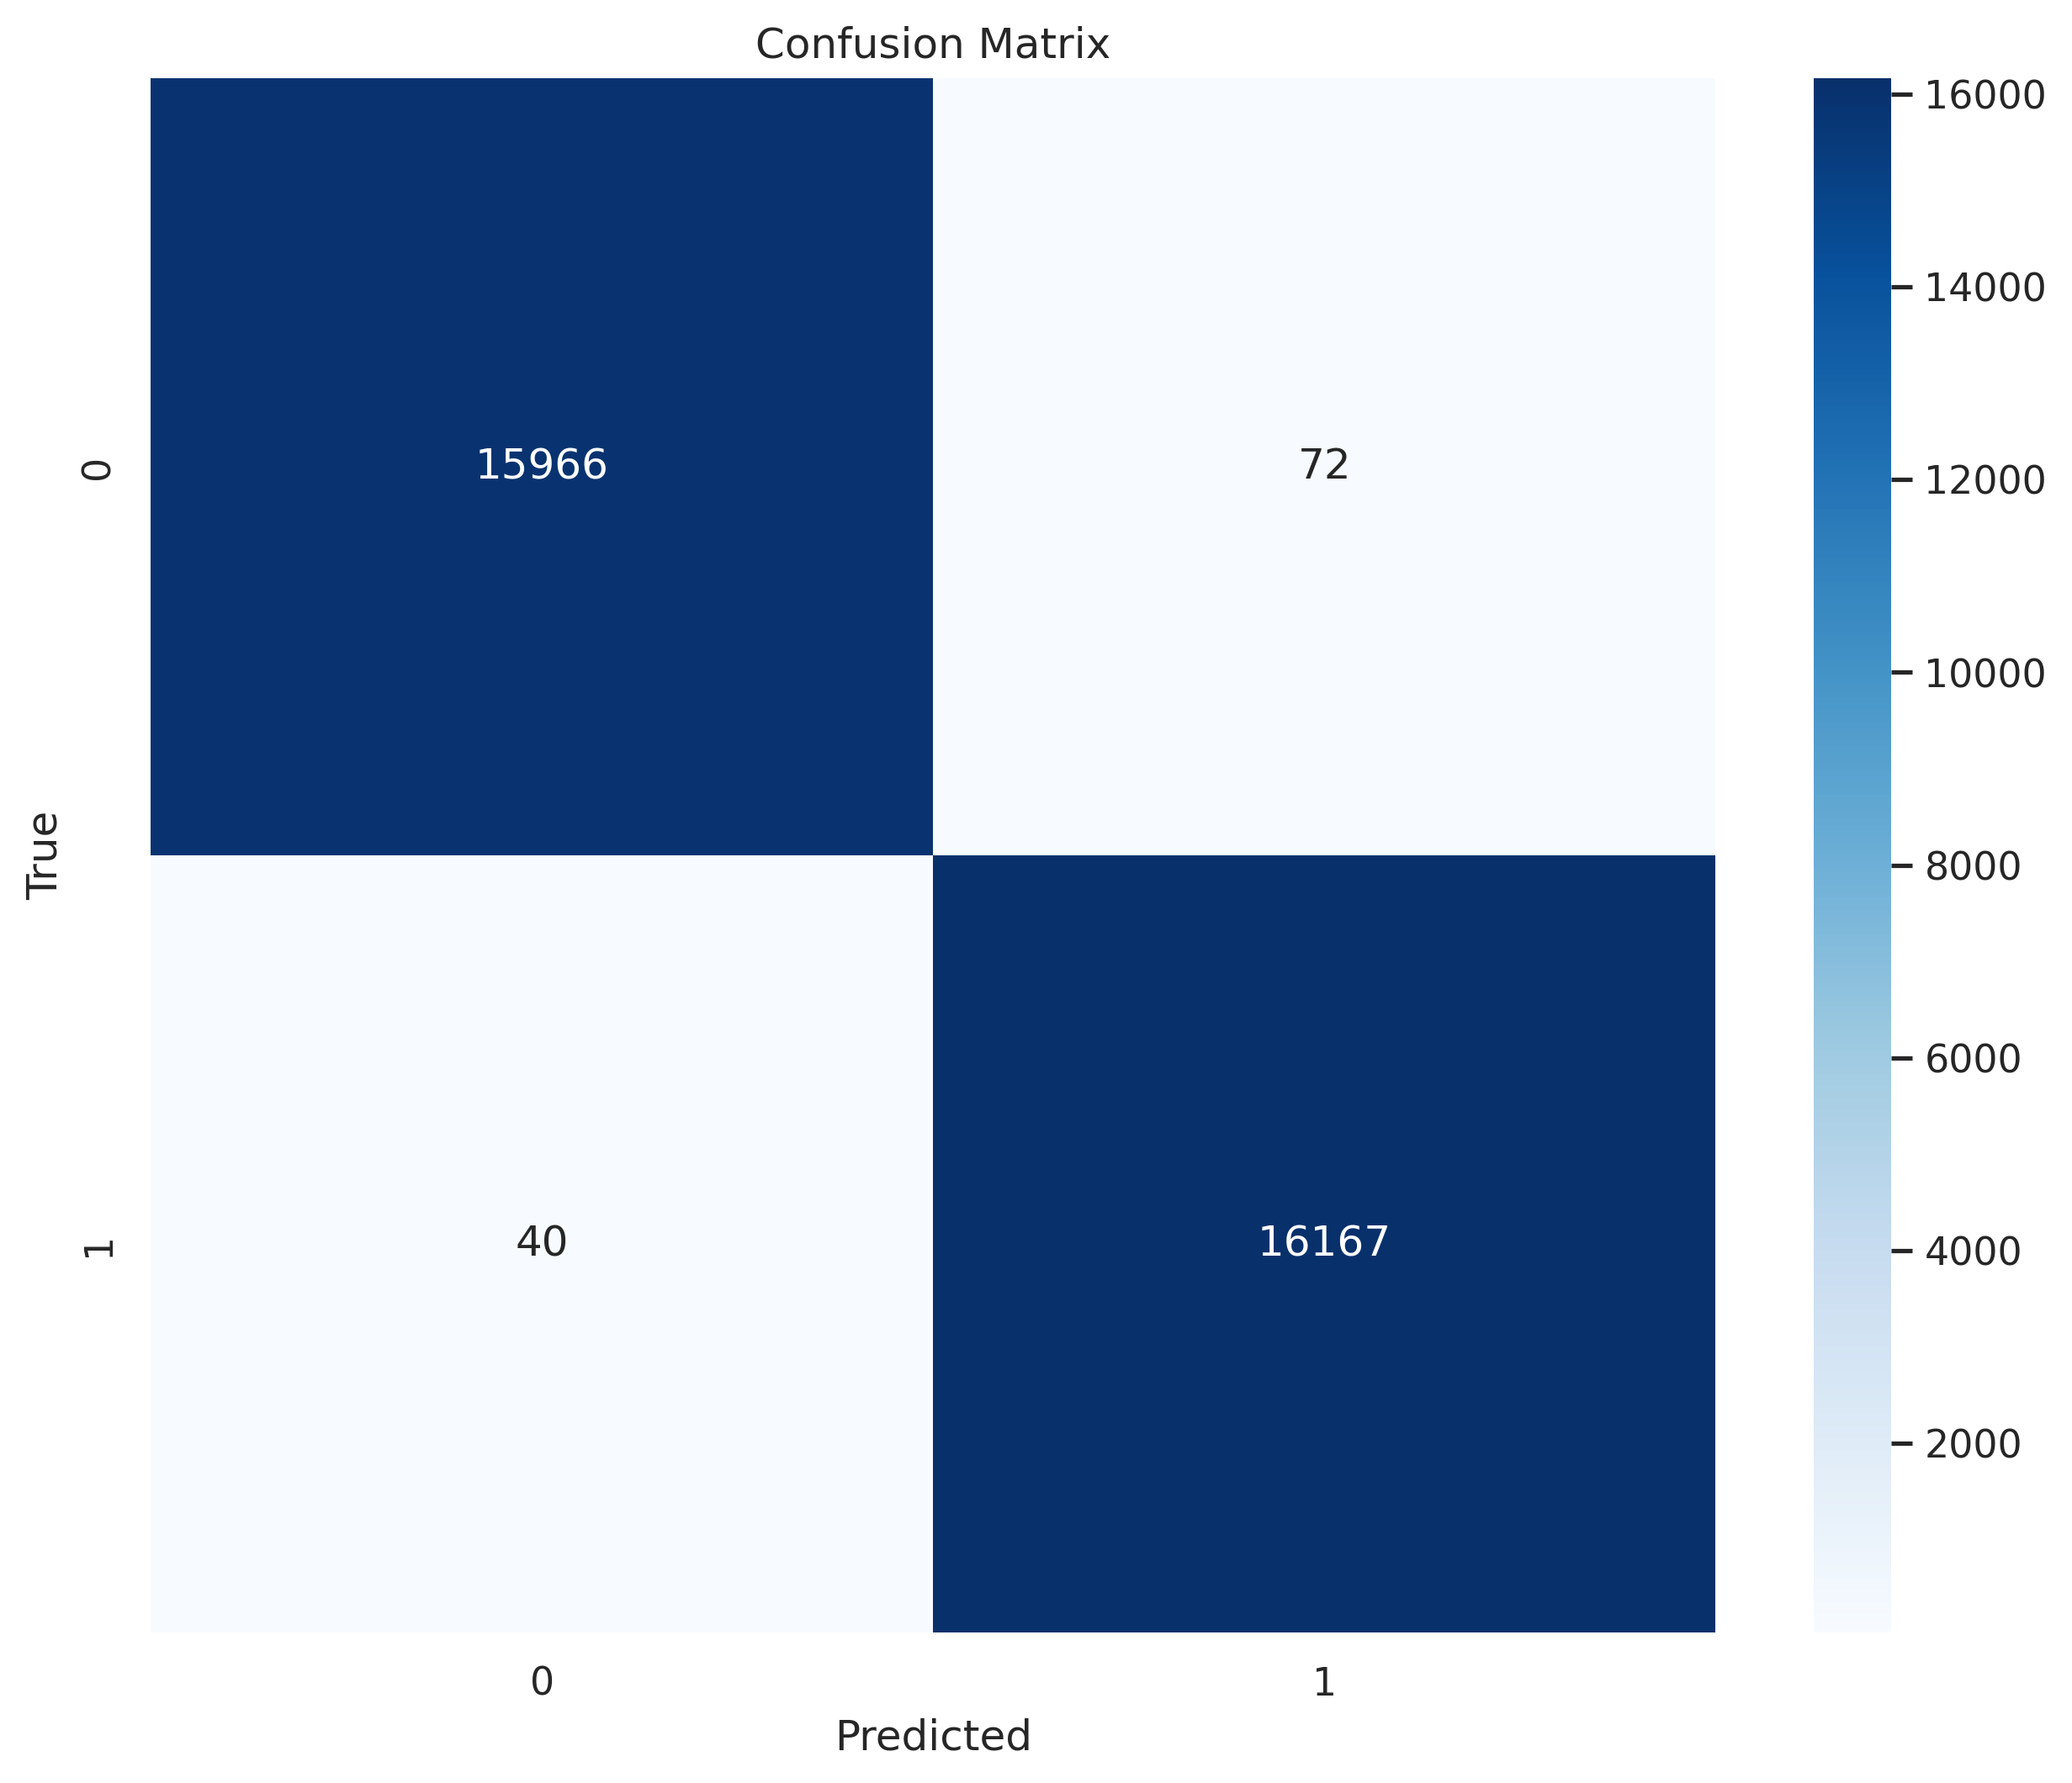
\includegraphics[width=0.8\textwidth]{images/dqn_nn_confusion_matrix.png}
    \caption{DQN-MLP confusion matrix.}
    \label{fig:dqn_nn_confusion}
\end{figure}

\vspace{0.5cm}

\begin{figure}[htbp]
    \centering
    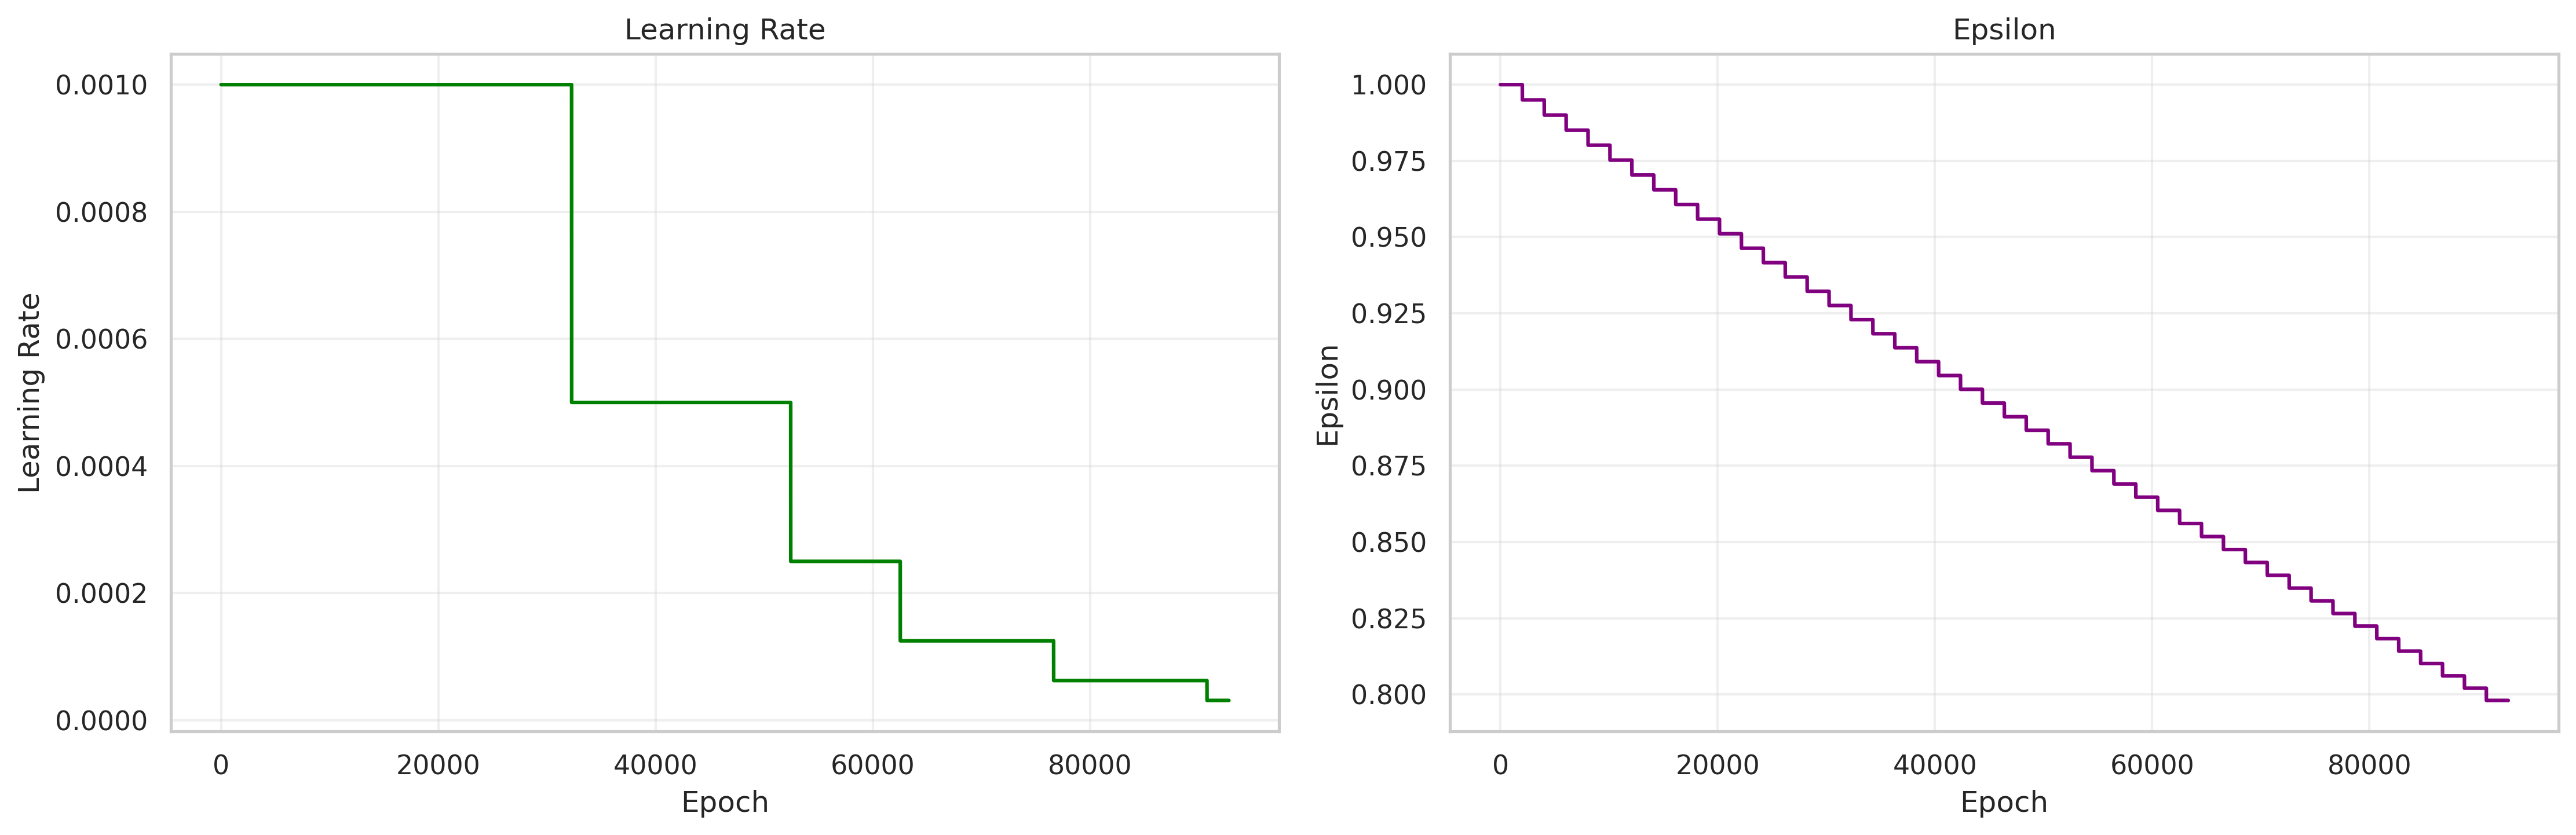
\includegraphics[width=0.8\textwidth]{images/dqn_nn_lr_epsilon.png}
    \caption{DQN-MLP learning rate and epsilon decay.}
    \label{fig:dqn_nn_lr_epsilon}
\end{figure}

\vspace{0.5cm}

\begin{figure}[htbp]
    \centering
    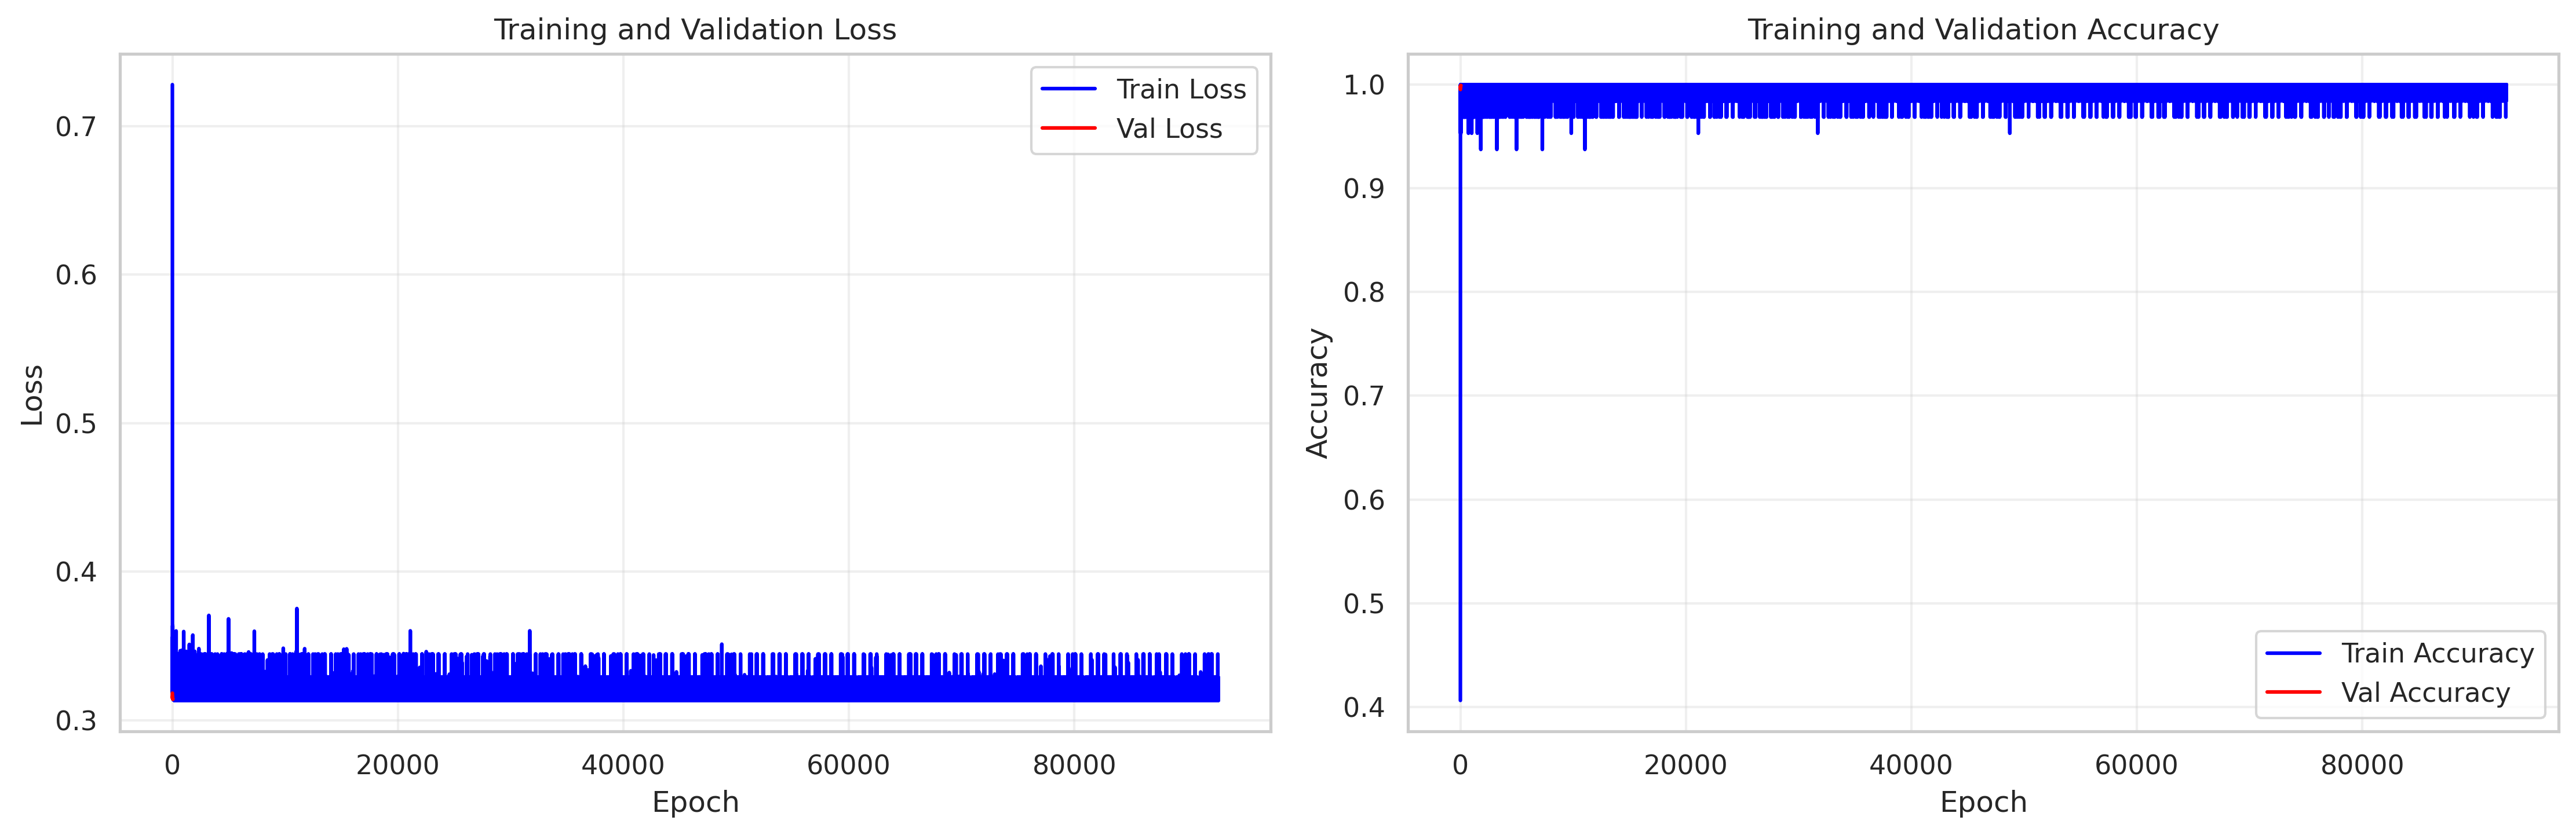
\includegraphics[width=0.8\textwidth]{images/dqn_nn_training_curves.png}
    \caption{DQN-MLP training curves.}
    \label{fig:dqn_nn_training_curves}
\end{figure}


\subsection{Results of MLP-DDQN}
To address the potential overestimation of Q-values inherent in the standard DQN algorithm, we also evaluated a Double DQN (DDQN) agent, which uses a decoupled action selection and evaluation mechanism. This model used the same MLP architecture as the standard DQN.

\begin{table}[H]
    \centering
    \caption{Binary Classification Results for MLP-DDQN}
    \label{tab:binary_ddqn_results}
    \begin{tabular}{@{}lc@{}}
        \toprule
        \textbf{Metric} & \textbf{Score} \\
        \midrule
        Accuracy & 0.9962474802294929 \\
        Precision & 0.9962559692934441 \\
        Recall & 0.9962474802294929 \\
        F1-Score & 0.9962516747433872 \\
        \bottomrule
    \end{tabular}
\end{table}
\begin{figure}[htbp]
    \centering
    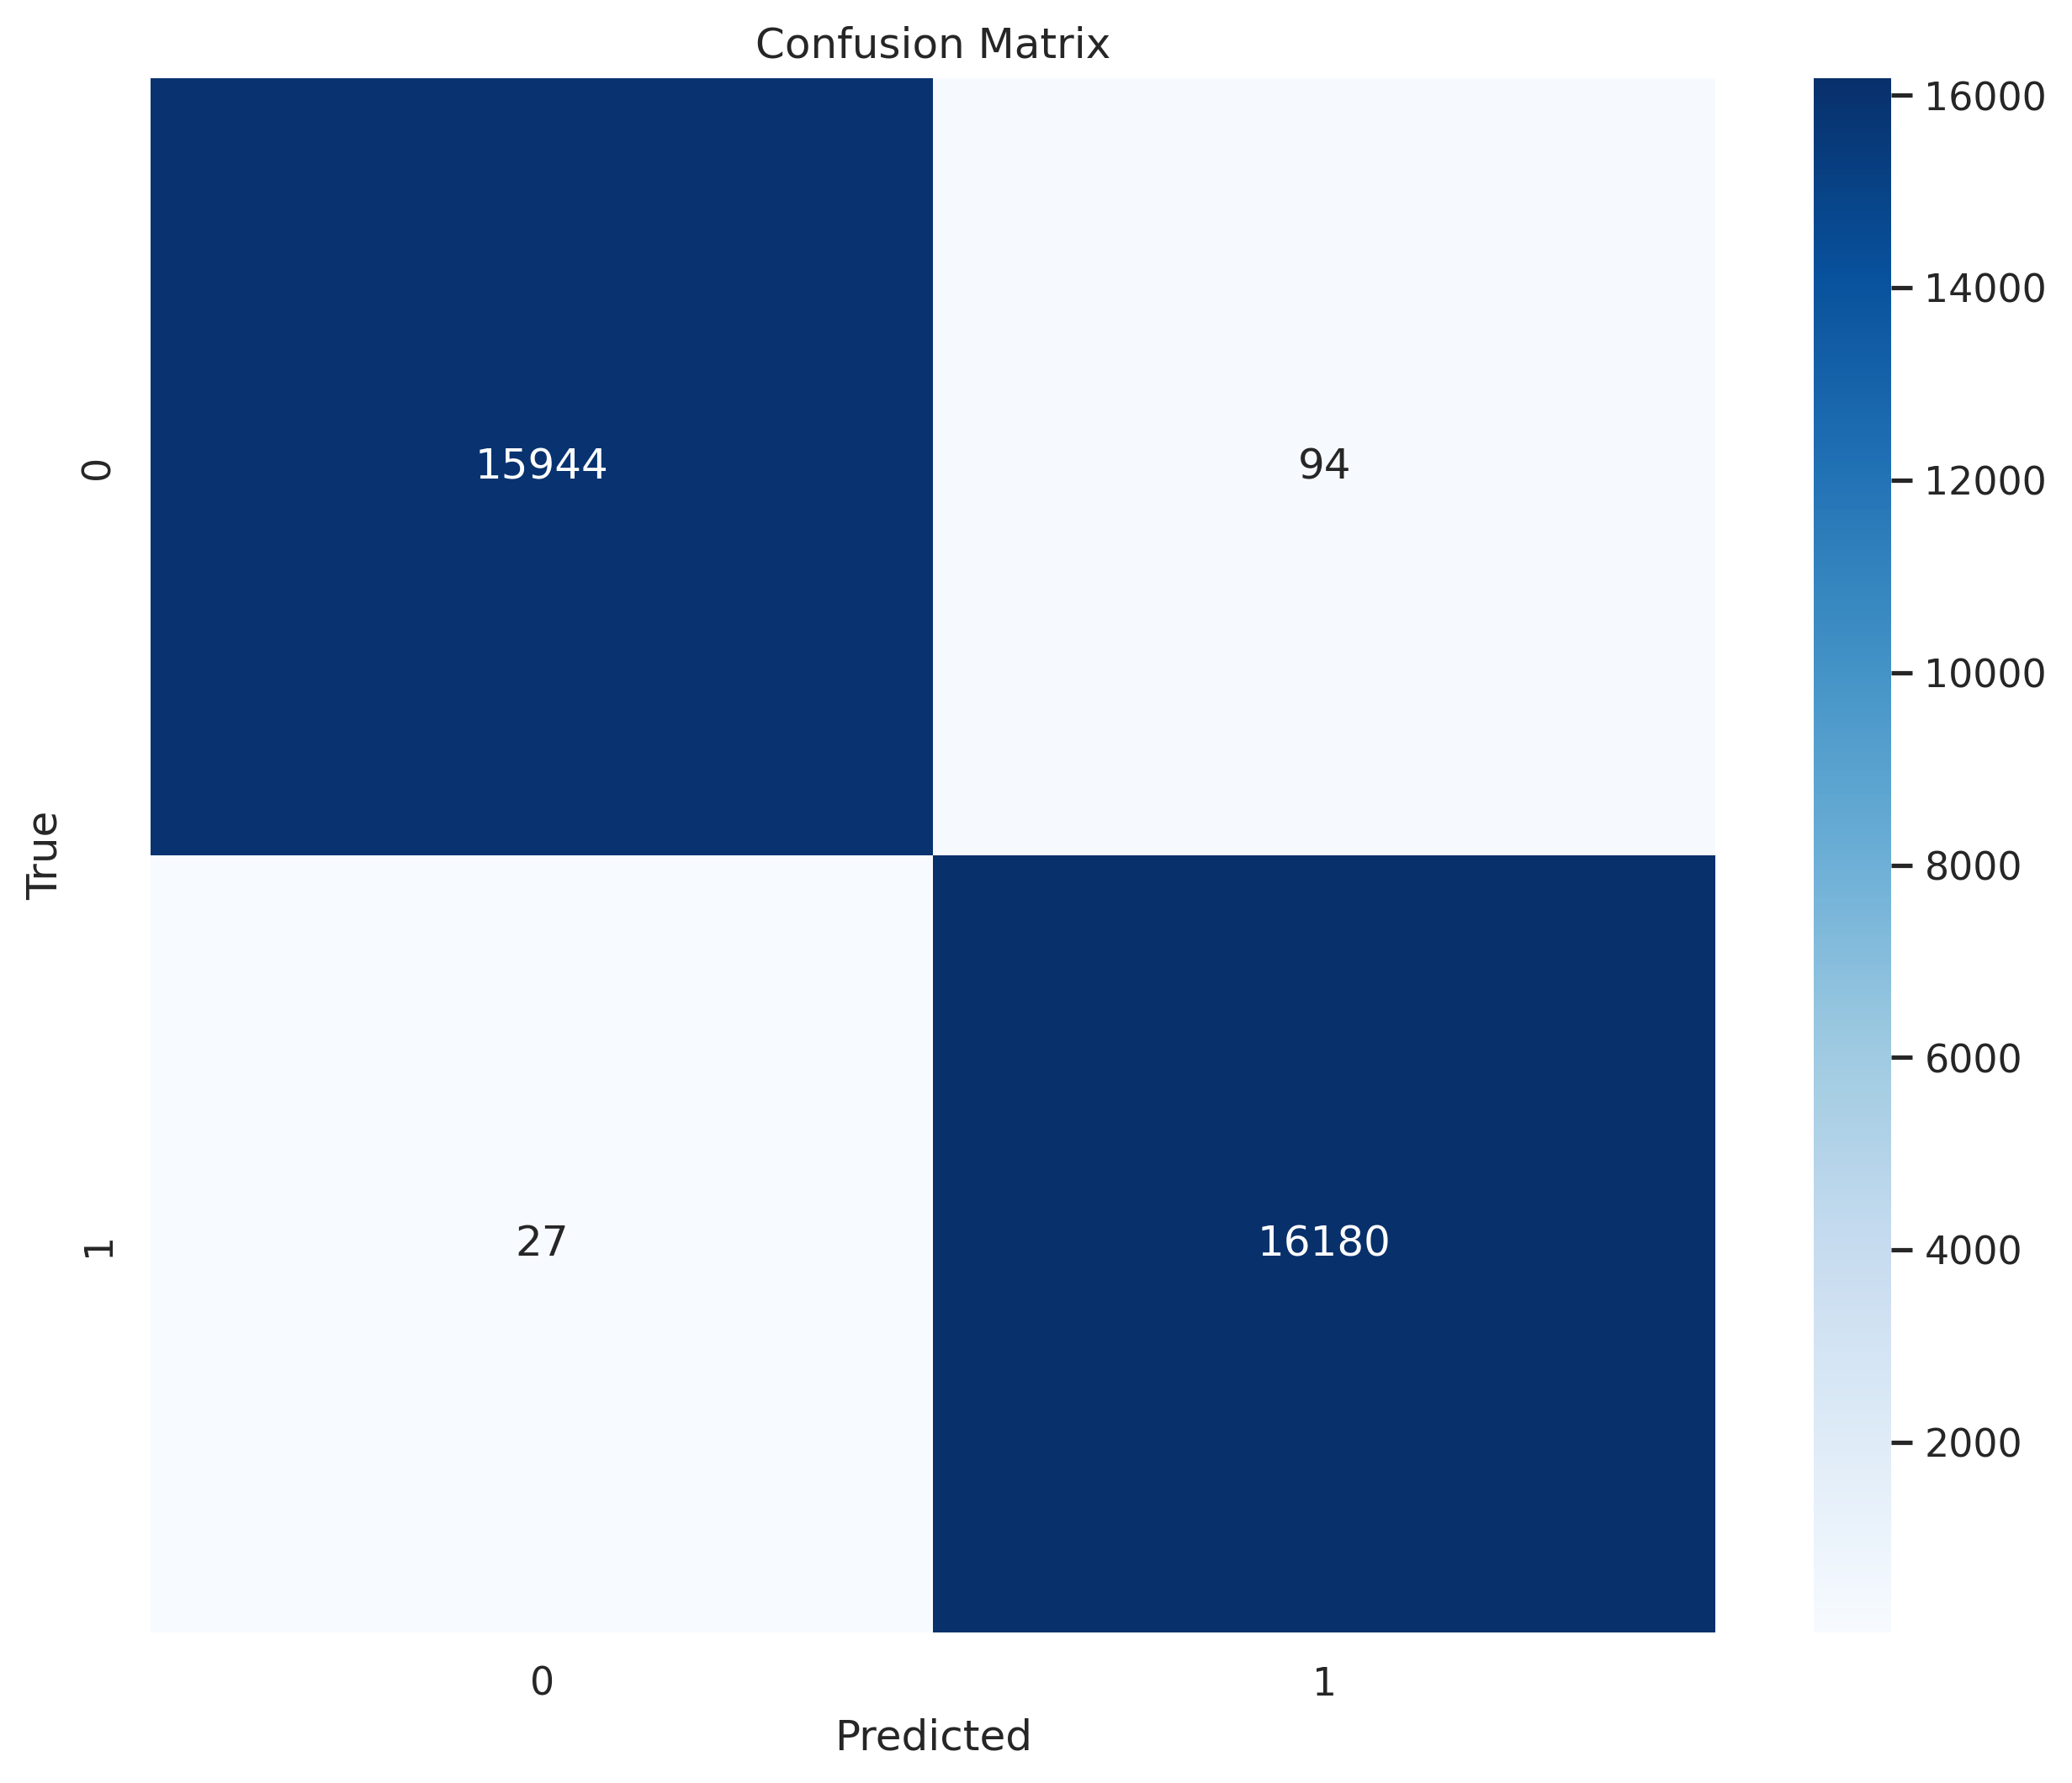
\includegraphics[width=0.7\textwidth]{images/double_dqn_nn_confusion_matrix.png}
    \caption{DDQN-MLP confusion matrix.}
    \label{fig:ddqn_nn_confusion}
\end{figure}

\vspace{0.5cm}

\begin{figure}[htbp]
    \centering
    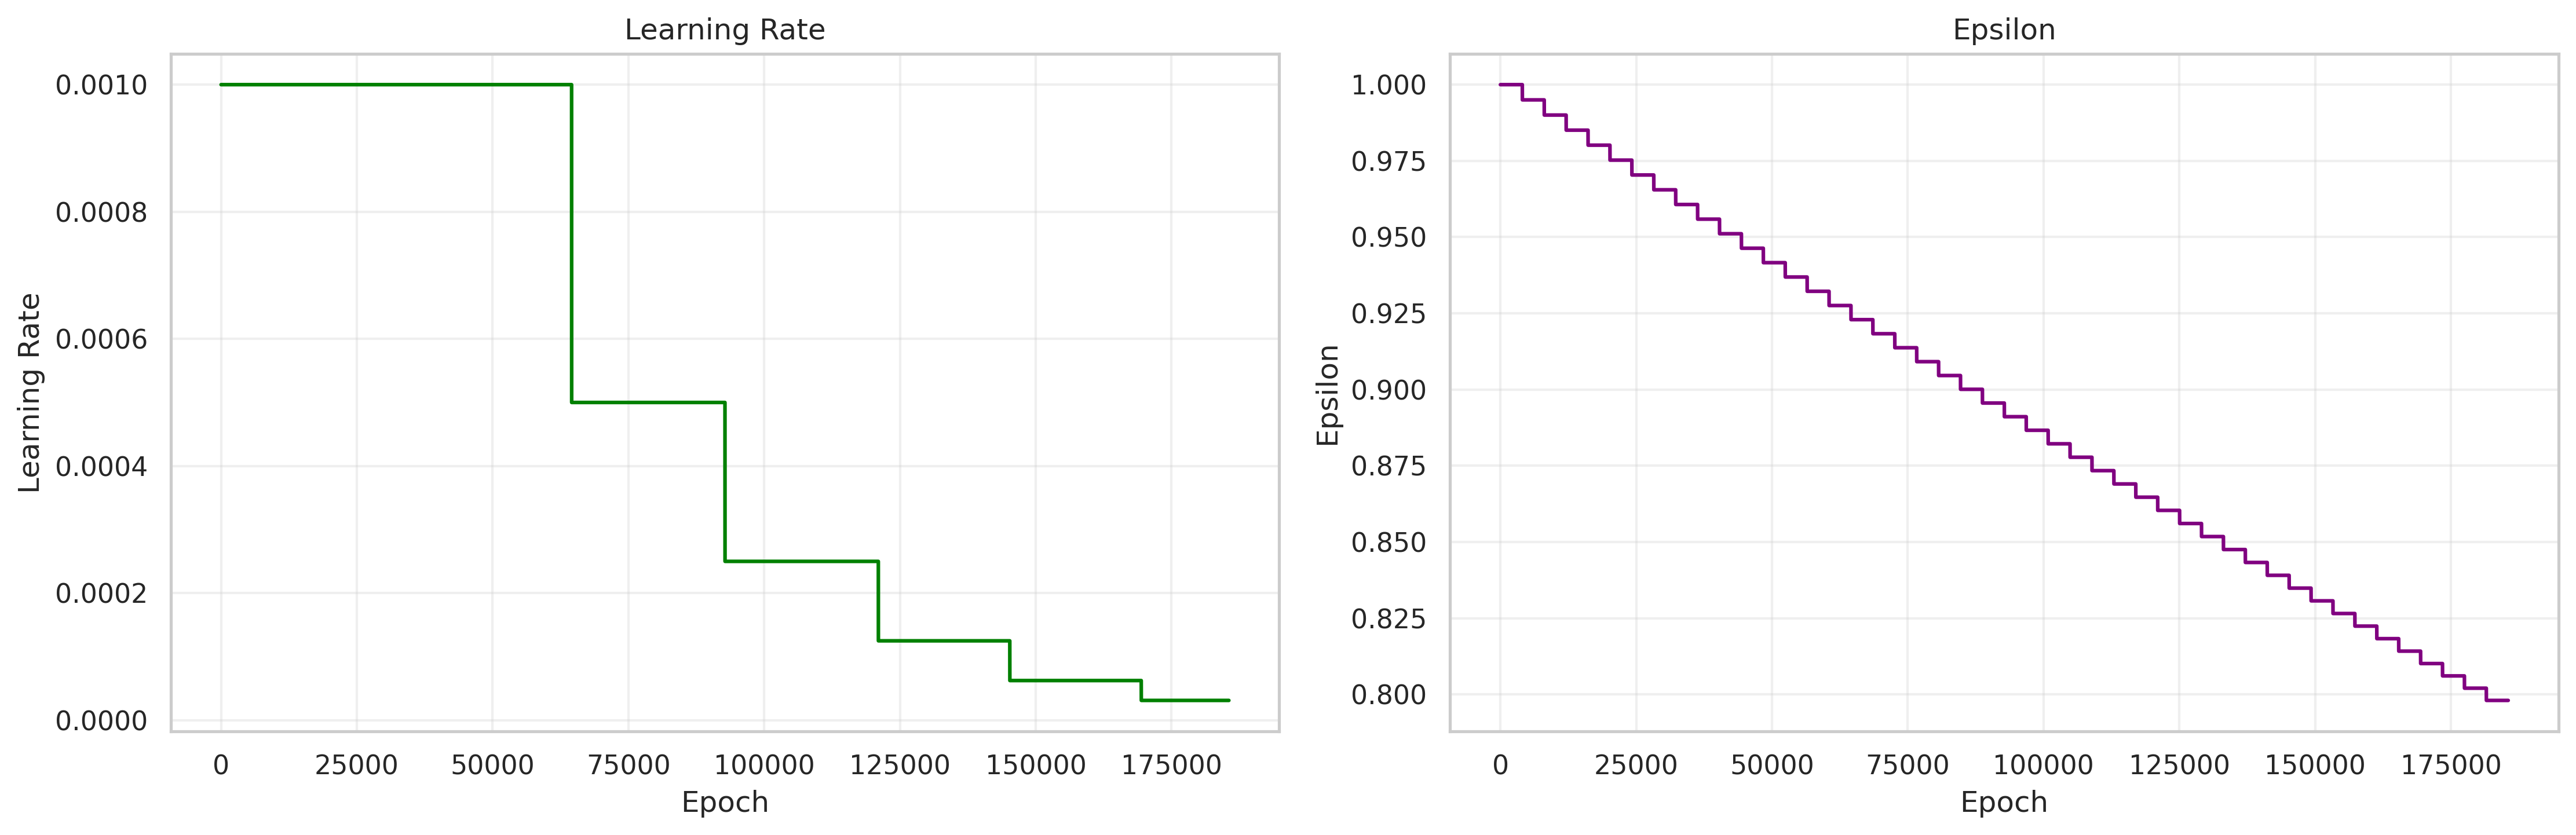
\includegraphics[width=0.7\textwidth]{images/double_dqn_nn_lr_epsilon.png}
    \caption{DDQN-MLP learning rate and epsilon decay.}
    \label{fig:ddqn_nn_lr_epsilon_nn}
\end{figure}

\vspace{0.5cm}

\begin{figure}[htbp]
    \centering
    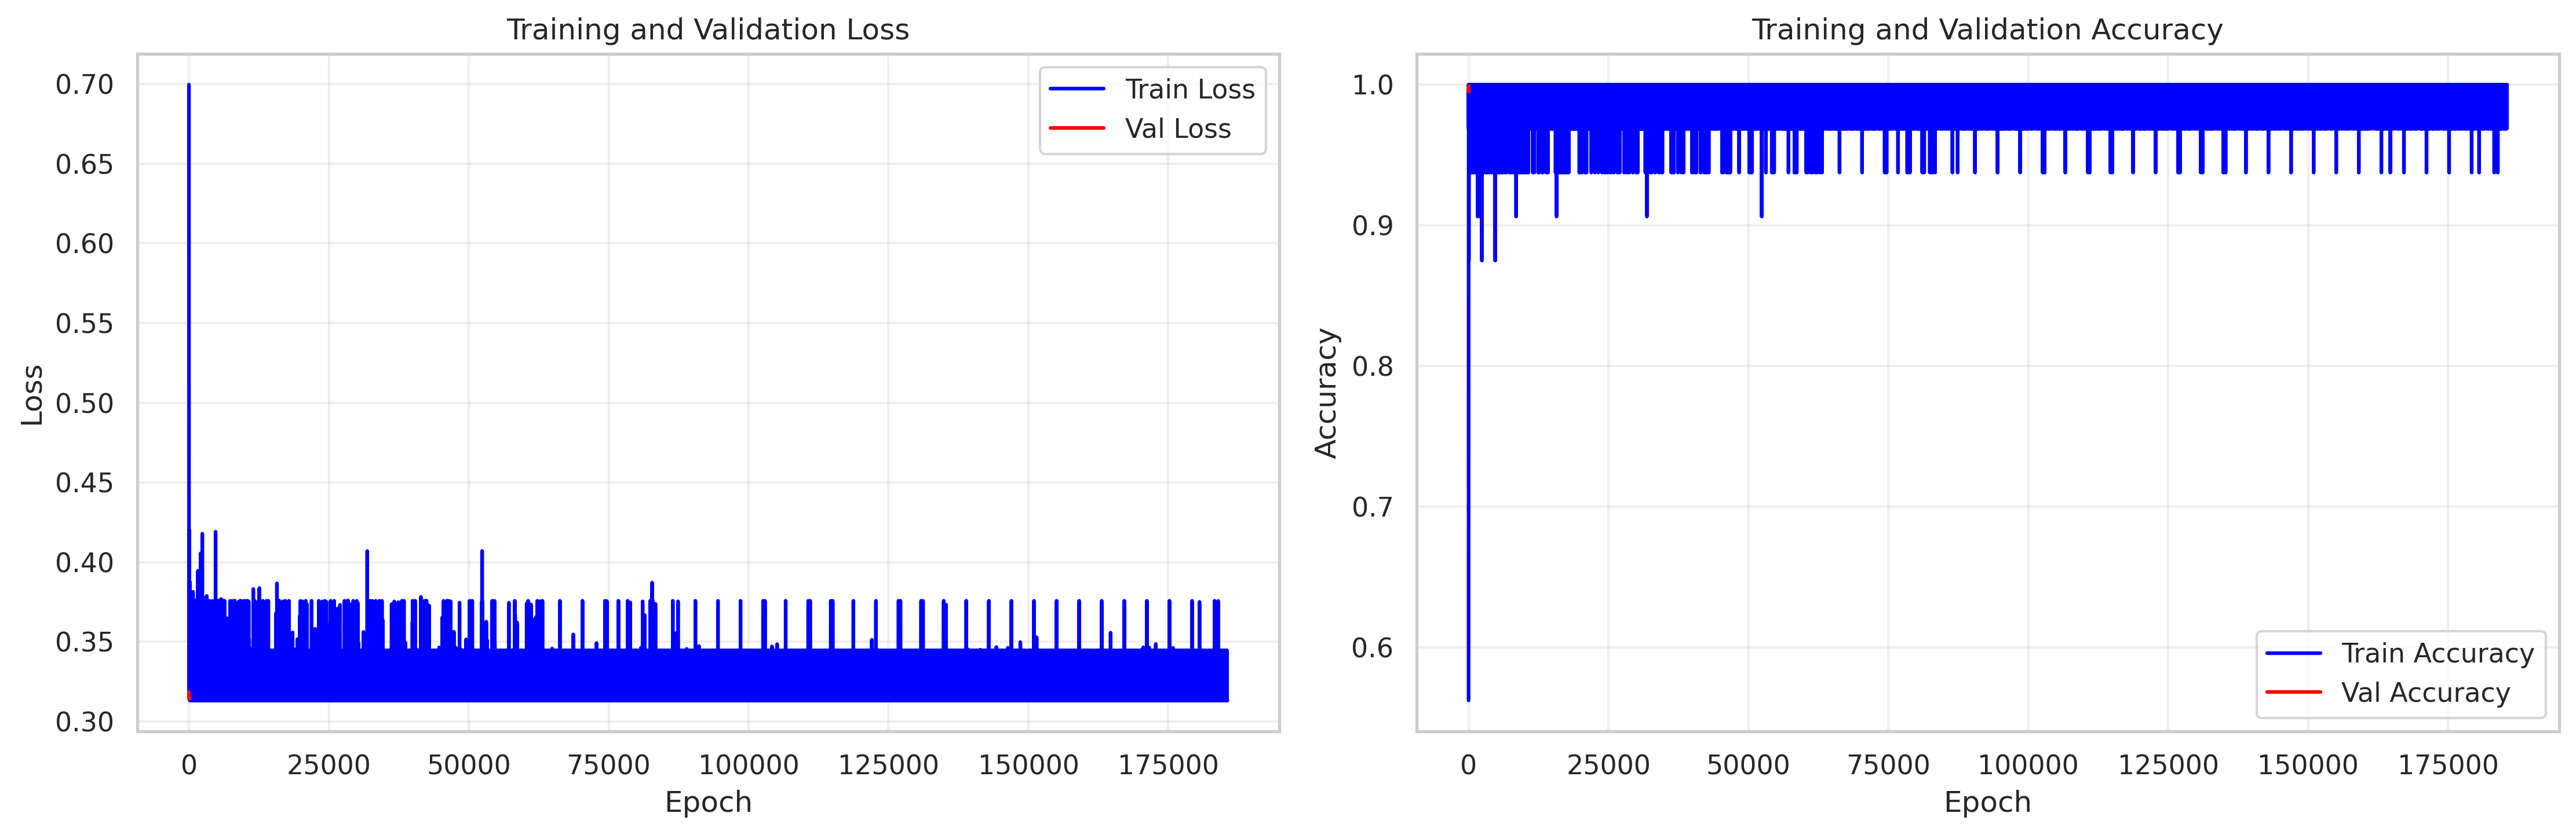
\includegraphics[width=0.7\textwidth]{images/double_dqn_nn_training_curves.png}
    \caption{DDQN-MLP training curves.}
    \label{fig:ddqn_nn_training_curves}
\end{figure}

The DDQN variant demonstrated a slight but consistent improvement across all metrics, achieving an F1-Score of 99.14 \%. This suggests that the more stable learning updates provided by the DDQN algorithm contribute to a more accurate and reliable final policy.

\newpage
\subsection{Results of CNN-DQN}
The CNN-based DQN agent was evaluated to test the hypothesis that spatial patterns within the feature-image representation could lead to superior performance. The results are shown in Table \ref{tab:binary_cnn_dqn_results}.

\begin{table}[H]
    \centering
    \caption{Binary Classification Results for CNN-DQN}
    \label{tab:binary_cnn_dqn_results}
    \begin{tabular}{@{}lc@{}}
        \toprule
        \textbf{Metric} & \textbf{Score} \\
        \midrule
        Accuracy & 0.9990702575386617 \\
        Precision & 0.9990703826387416 \\
        Recall & 0.9990702575386617 \\
        F1-Score & 0.9990702586745697 \\
        \bottomrule
    \end{tabular}
\end{table}

\begin{figure}[htbp]
    \centering
    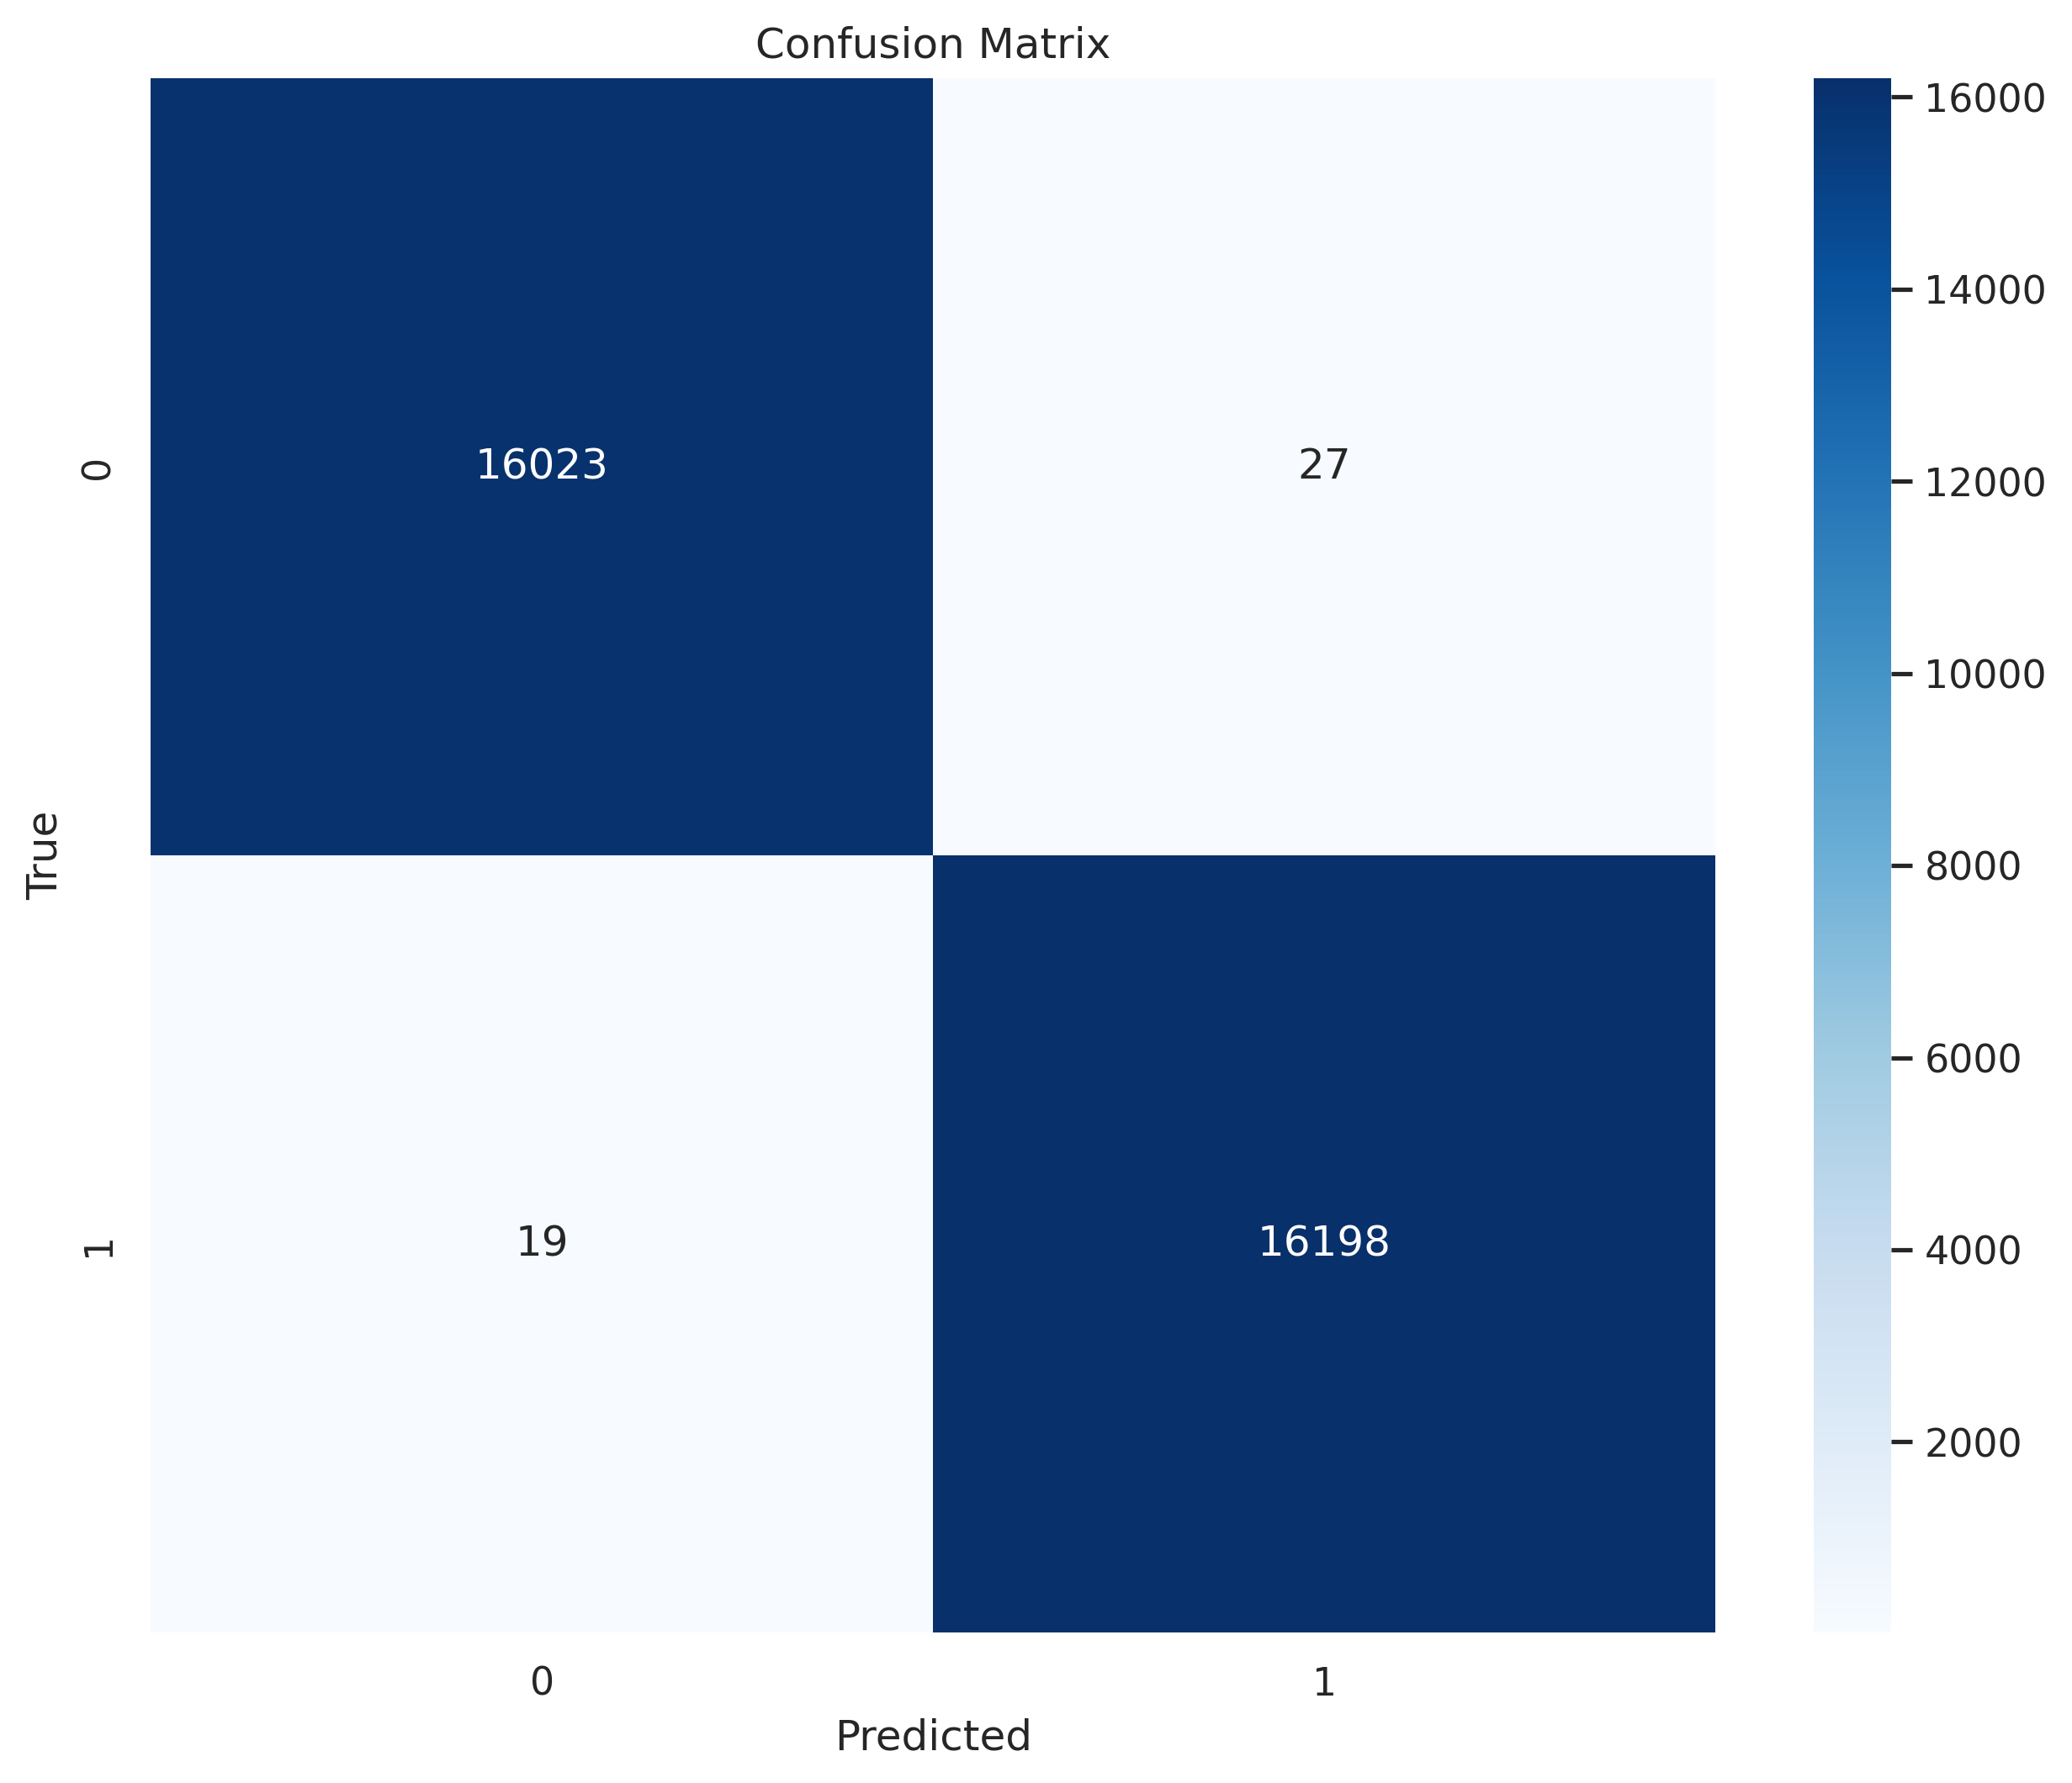
\includegraphics[width=0.7\textwidth]{images/dqn_cnn_confusion_matrix.png}
    \caption{DQN-CNN confusion matrix.}
    \label{fig:dqn_cnn_confusion}
\end{figure}

\vspace{0.5cm}

\begin{figure}[htbp]
    \centering
    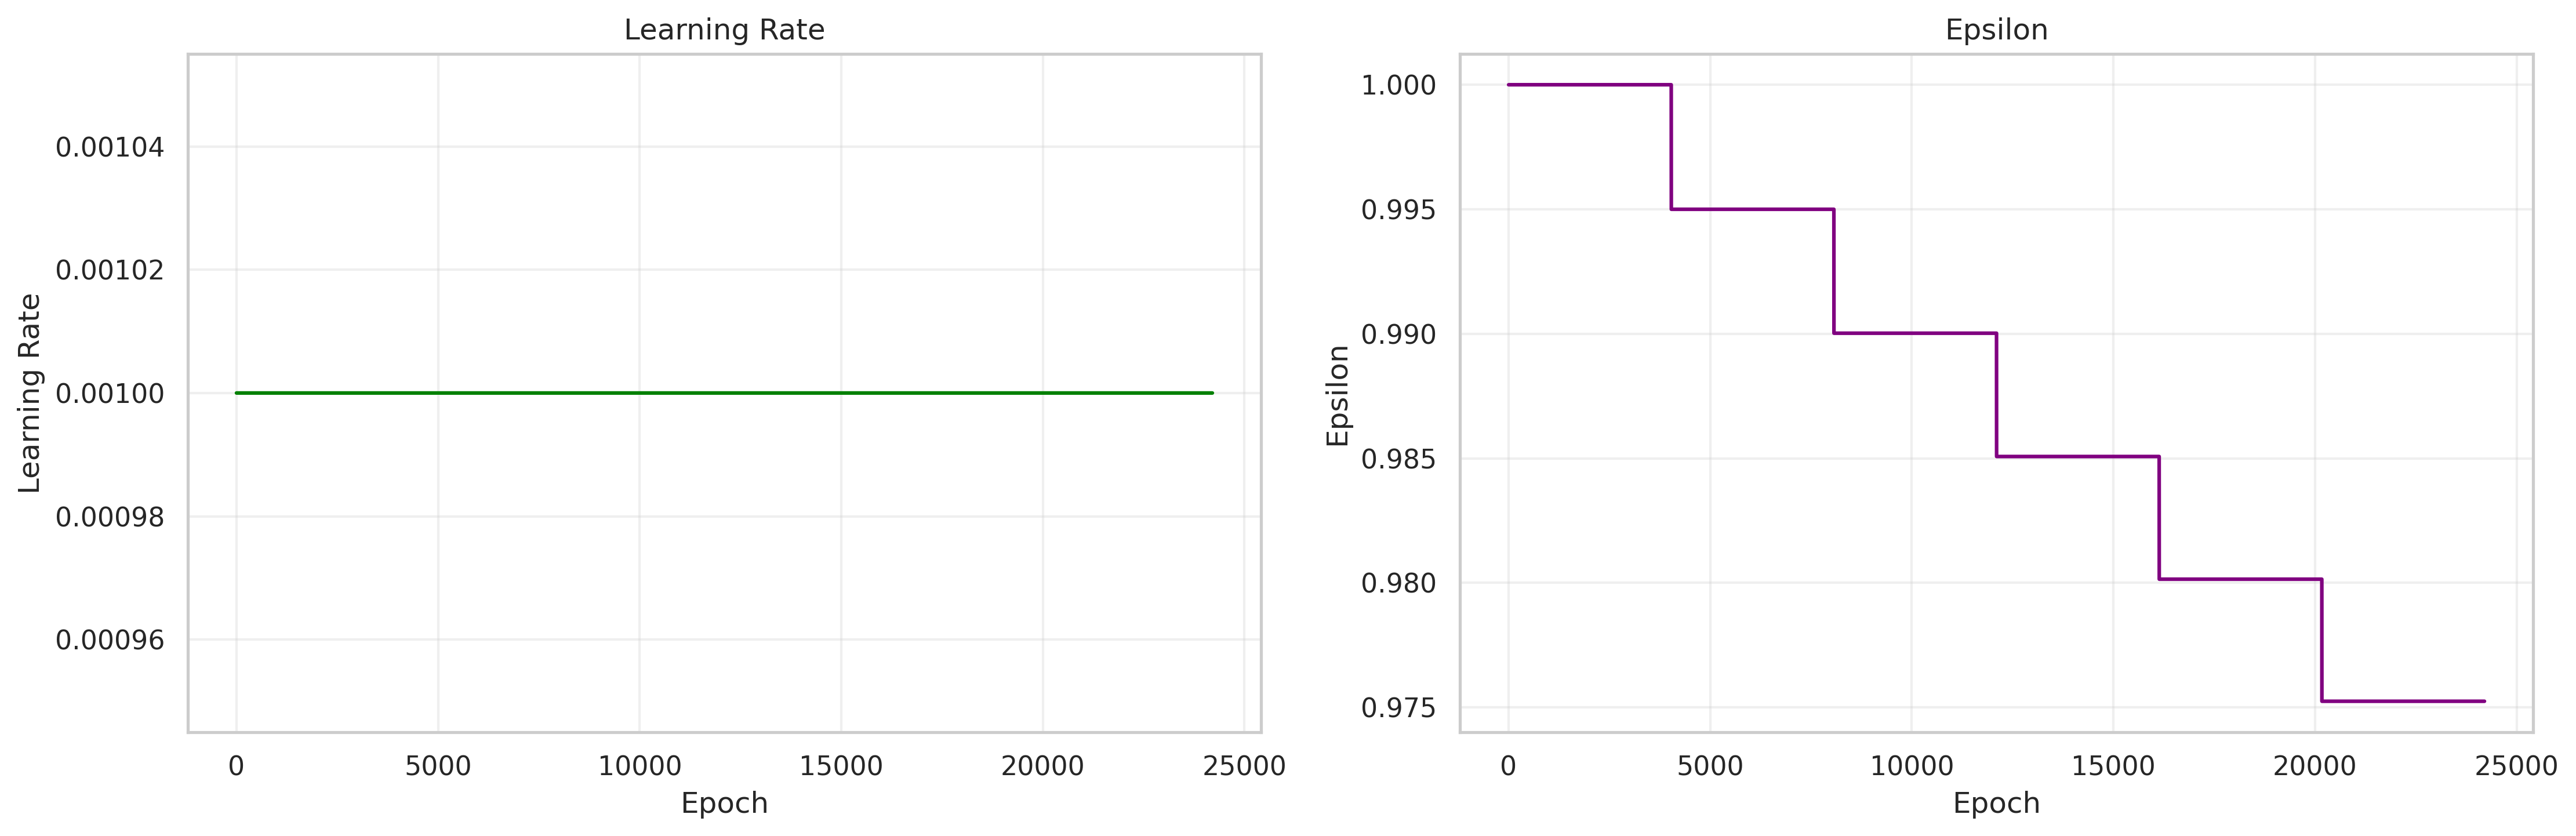
\includegraphics[width=0.7\textwidth]{images/dqn_cnn_lr_epsilon.png}
    \caption{DDQN-CNN learning rate and epsilon decay.}
    \label{fig:dqn_cnn_lr_epsilon_cnn}
\end{figure}

\vspace{0.5cm}

\begin{figure}[htbp]
    \centering
    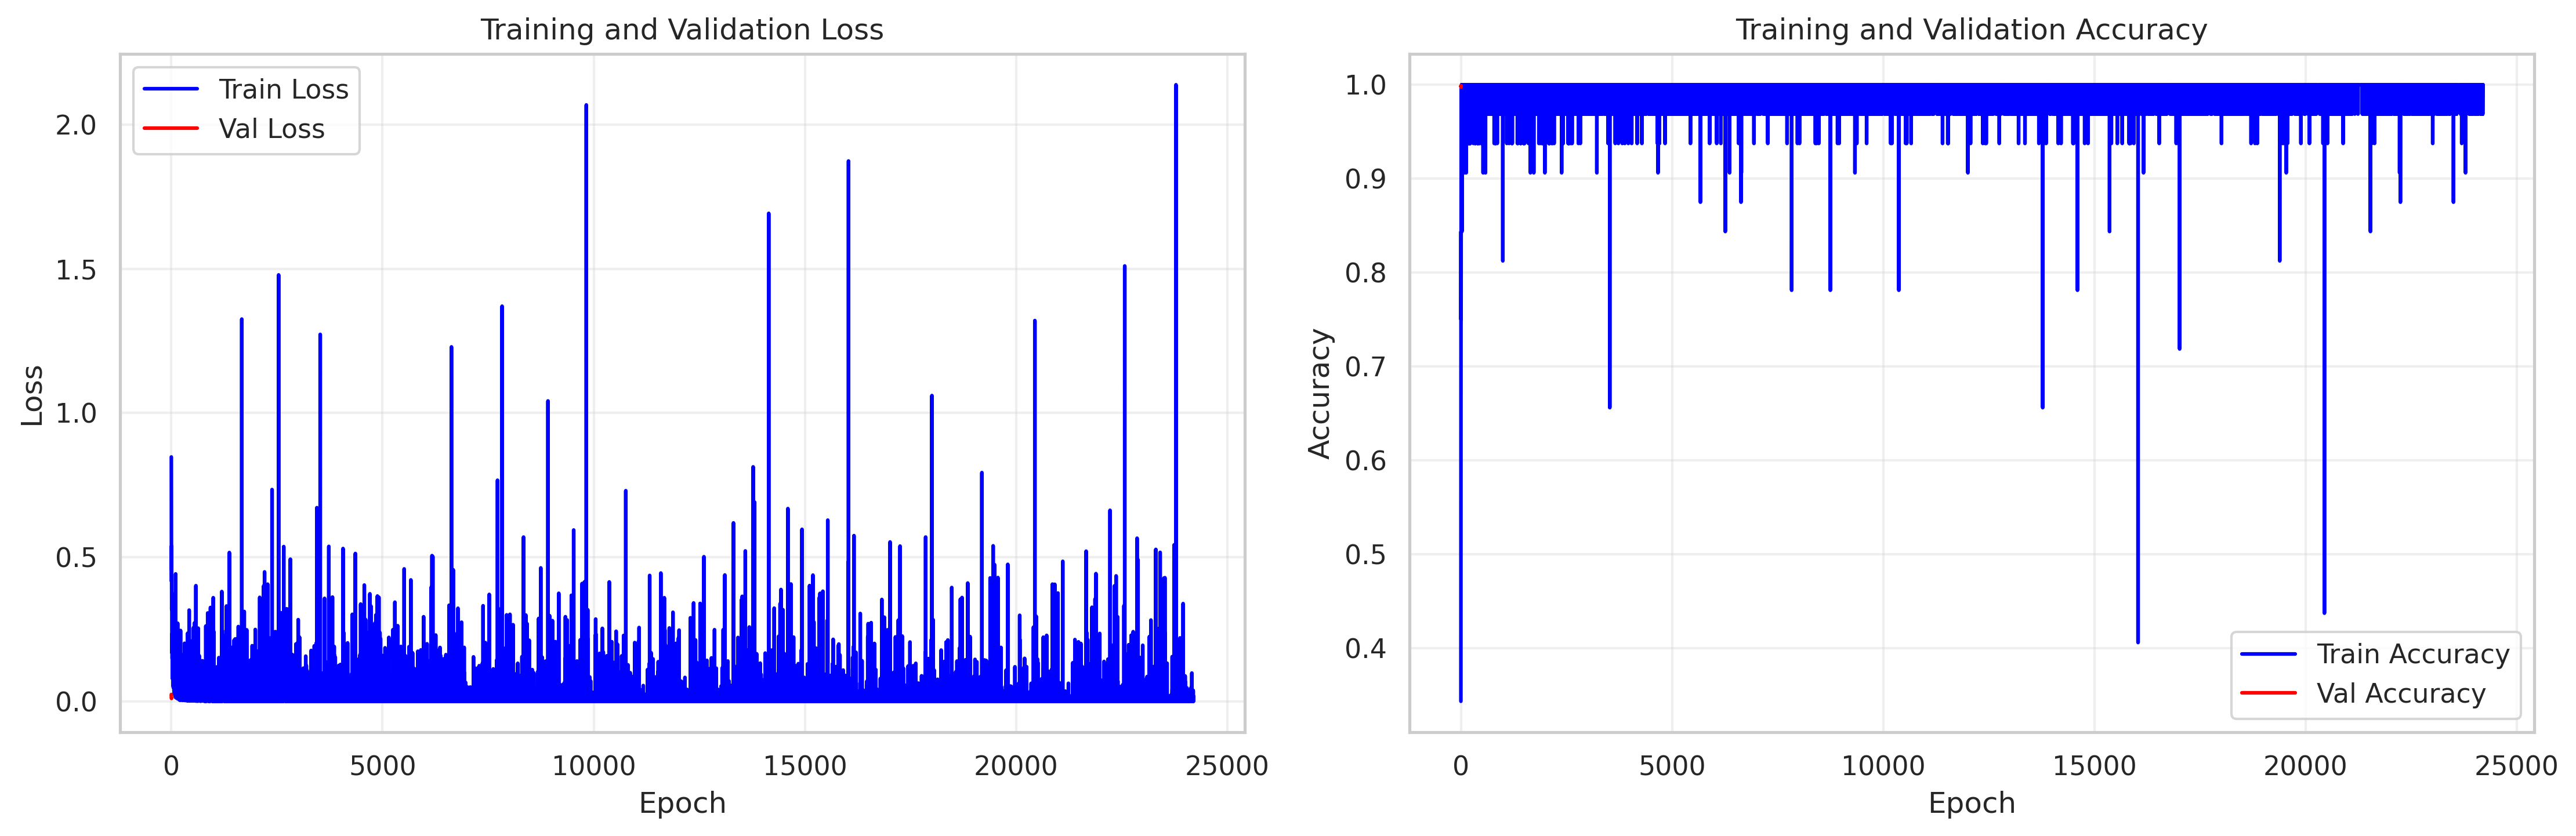
\includegraphics[width=0.7\textwidth]{images/dqn_cnn_training_curves.png}
    \caption{DDQN-CNN training curves.}
    \label{fig:dqn_cnn_training_curves}
\end{figure}

The CNN-DQN model emerged as the top performer in the binary classification task, with an impressive F1-Score of 99.46

\subsection{Results of CNN-DDQN}
The CNN-based DDQN agent was evaluated to test the hypothesis that spatial patterns within the feature-image representation could lead to superior performance. The results are shown in Table \ref{tab:binary_cnn_dqn_results}.

\begin{table}[H]
    \centering
    \caption{Binary Classification Results for CNN-DDQN}
    \label{tab:binary_cnn_ddqn_results}
    \begin{tabular}{@{}lc@{}}
        \toprule
        \textbf{Metric} & \textbf{Score} \\
        \midrule
        Accuracy & 0.9990082747079059 \\
        Precision & 0.9990083456349137 \\
        Recall & 0.9990082747079059 \\
        F1-Score & 0.9990082756280634 \\
        \bottomrule
    \end{tabular}
\end{table}

\begin{figure}[htbp]
    \centering
    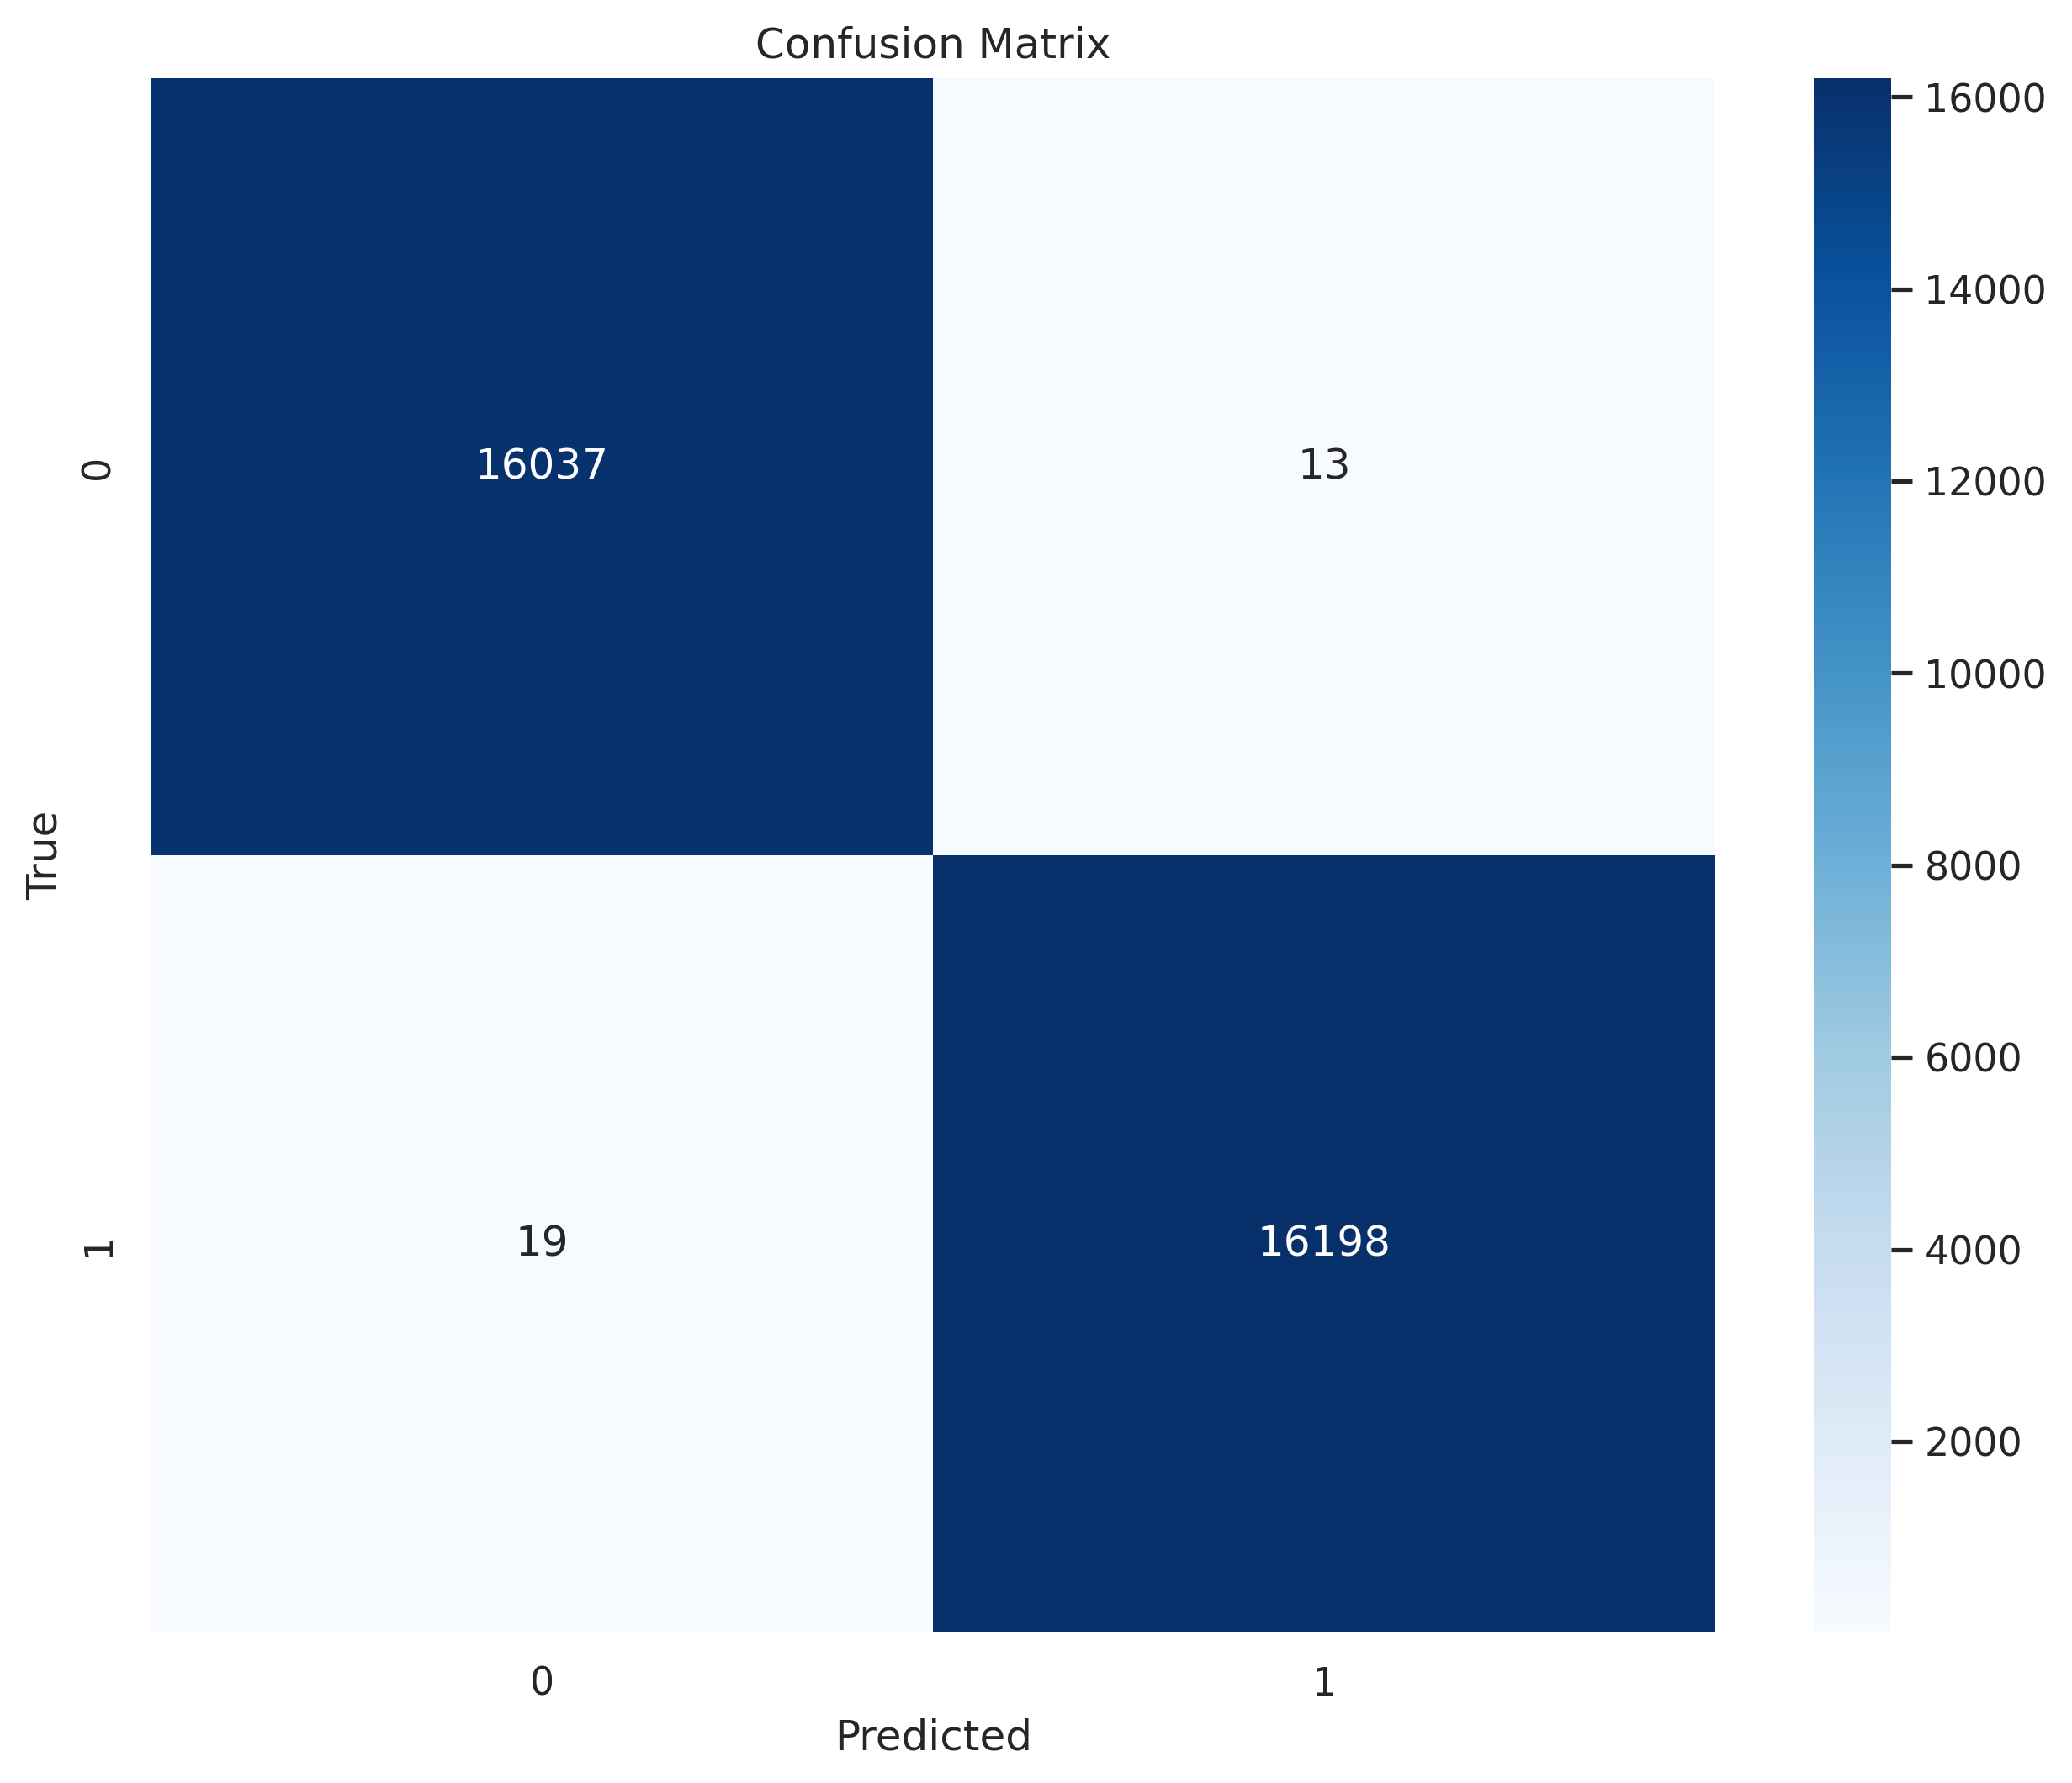
\includegraphics[width=0.7\textwidth]{images/double_dqn_cnn_confusion_matrix.png}
    \caption{DDQN-CNN confusion matrix.}
    \label{fig:ddqn_cnn_confusion}
\end{figure}

\vspace{0.5cm}

\begin{figure}[htbp]
    \centering
    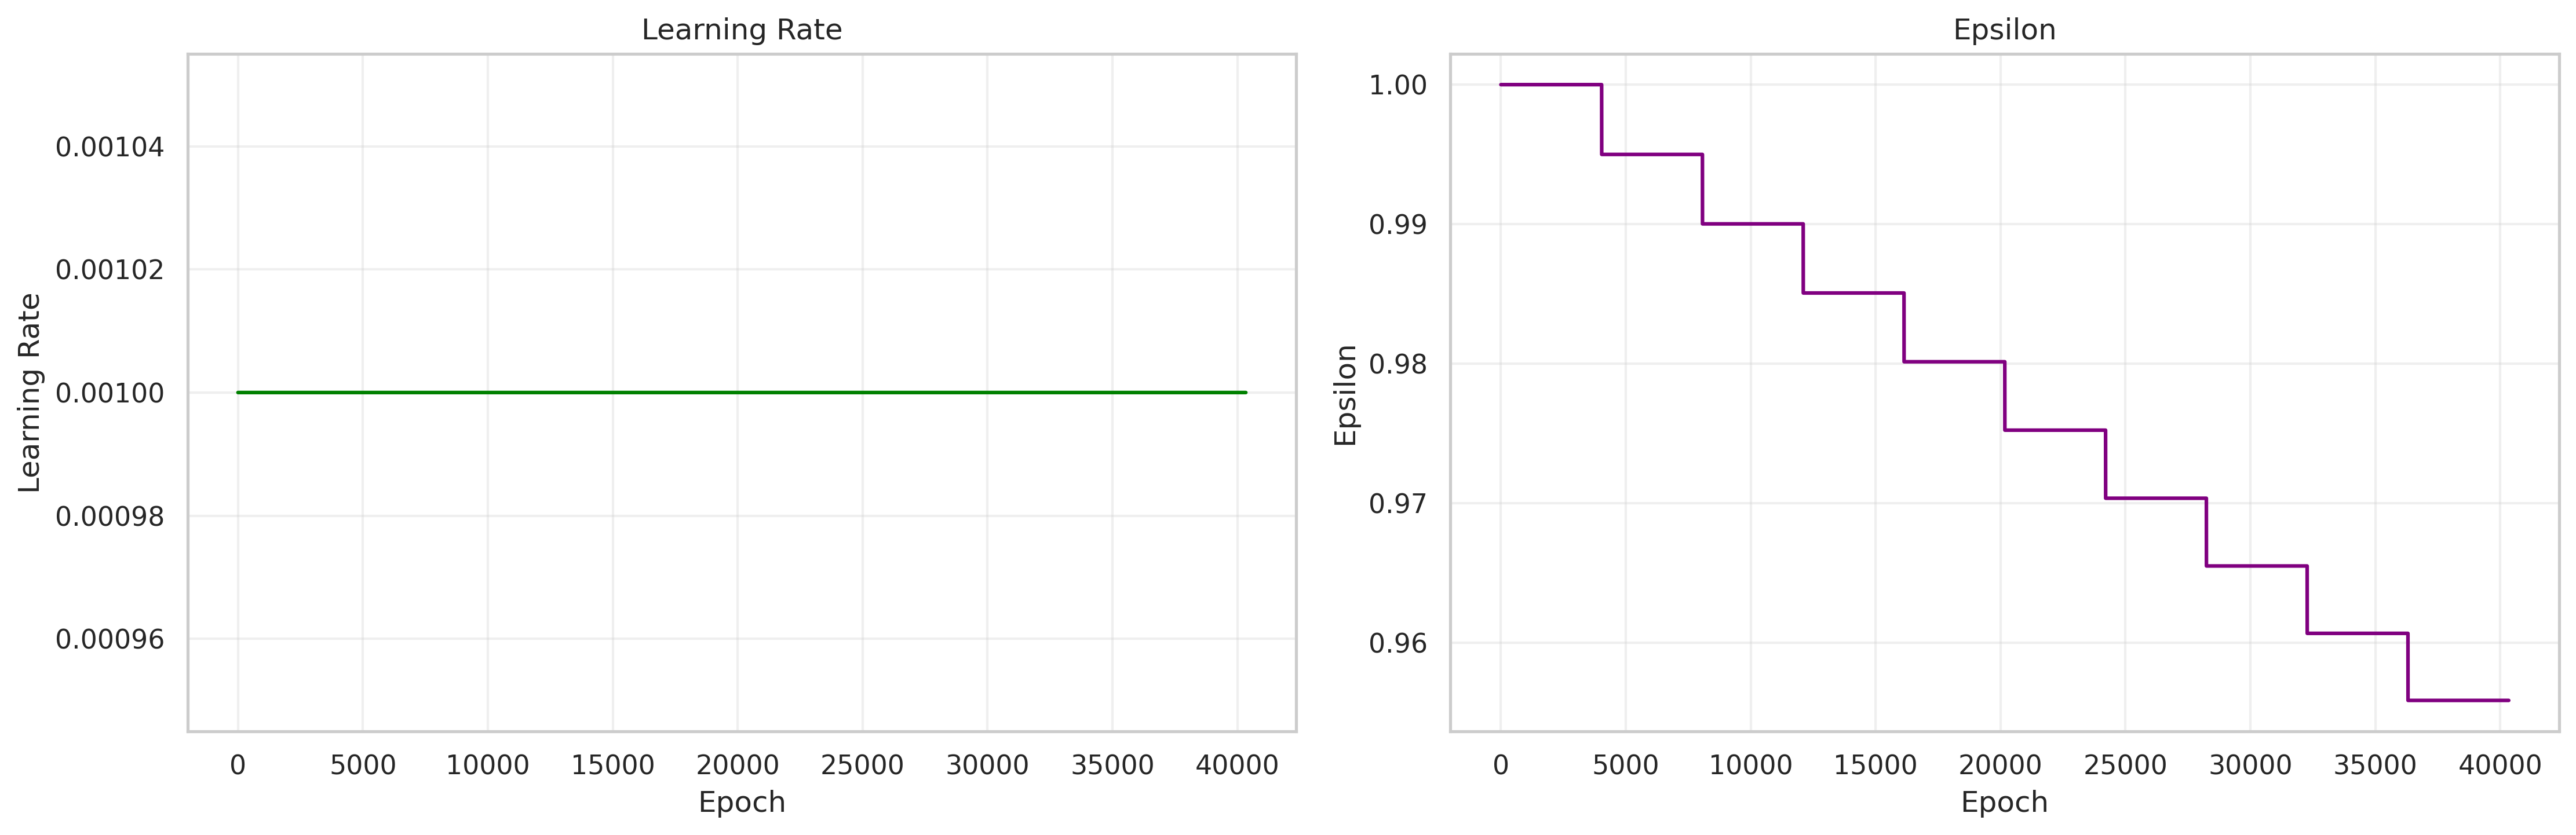
\includegraphics[width=0.7\textwidth]{images/double_dqn_cnn_lr_epsilon.png}
    \caption{DDQN-CNN learning rate and epsilon decay.}
    \label{fig:ddqn_cnn_lr_epsilon_cnn}
\end{figure}

\vspace{0.5cm}

\begin{figure}[htbp]
    \centering
    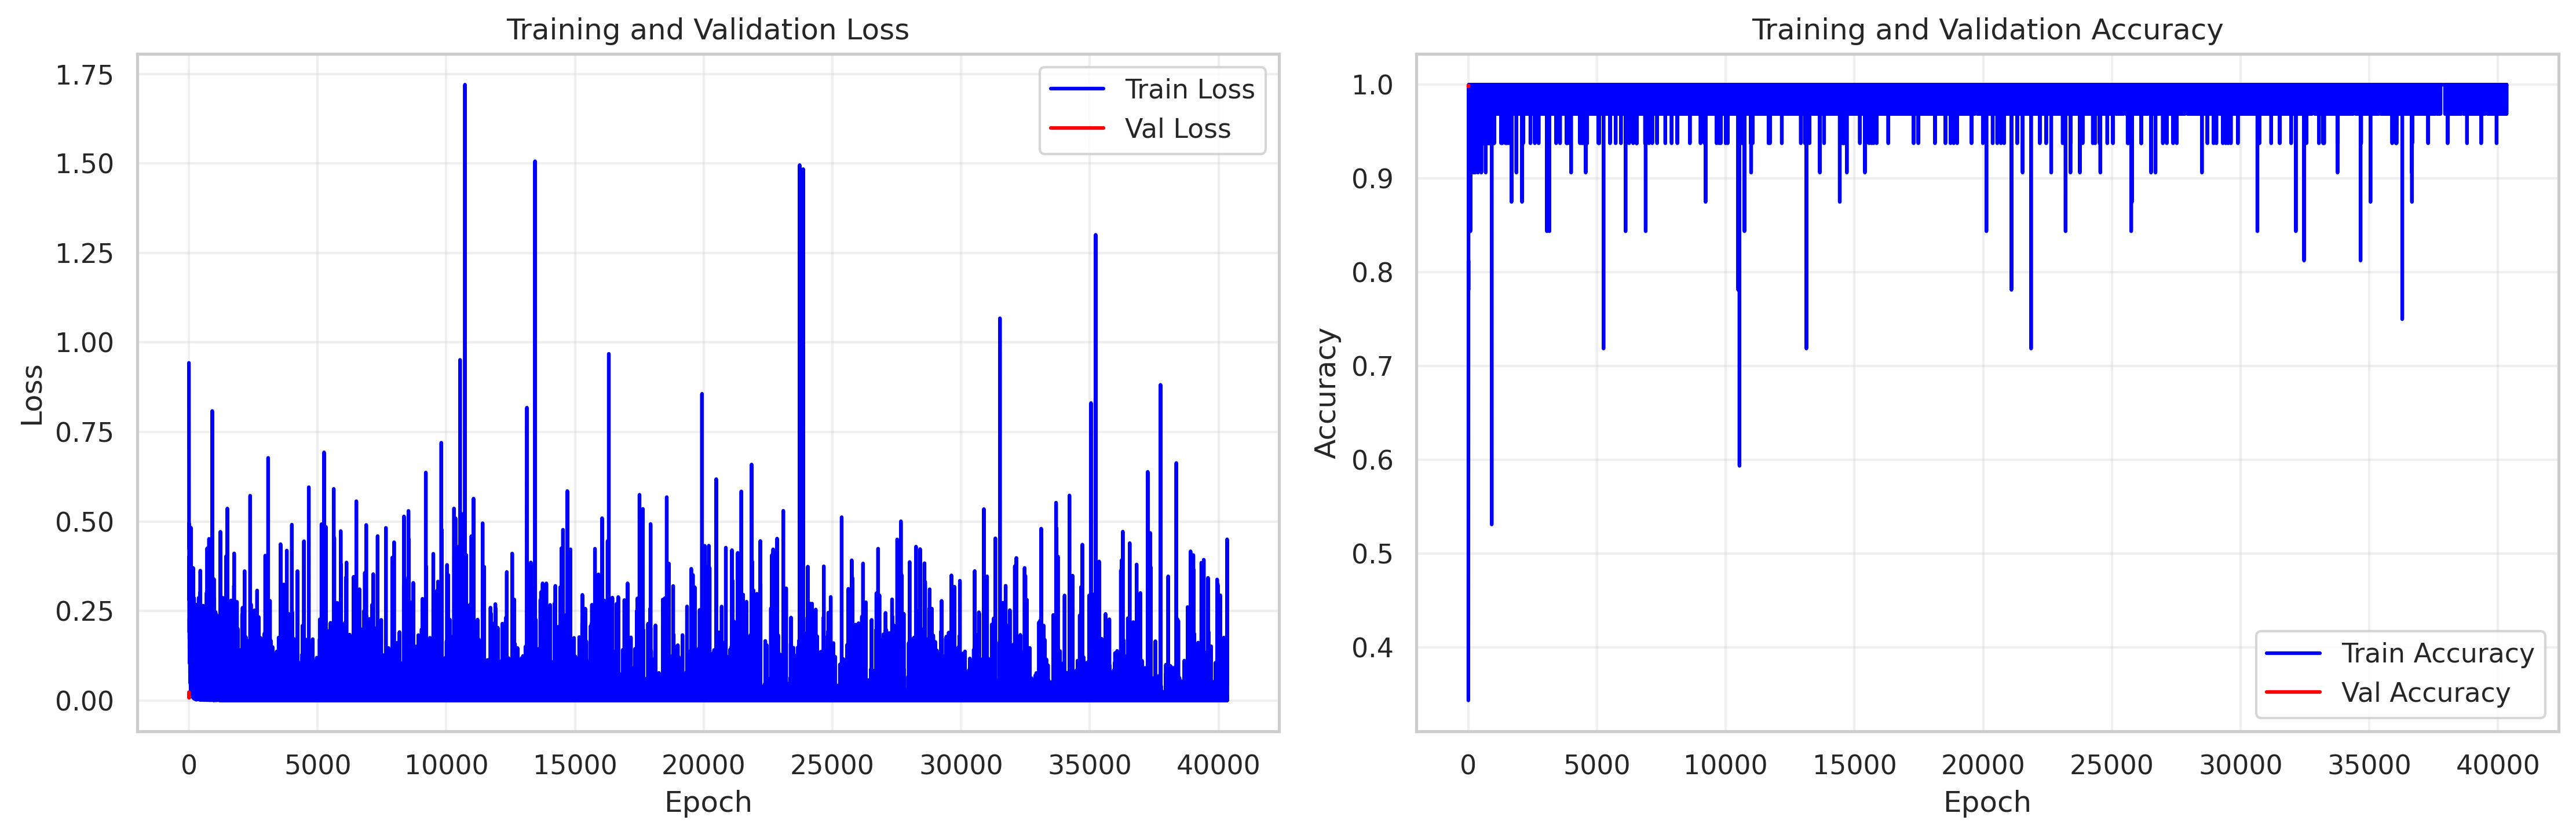
\includegraphics[width=0.7\textwidth]{images/double_dqn_cnn_training_curves.png}
    \caption{DDQN-CNN training curves.}
    \label{fig:ddqn_cnn_training_curves}
\end{figure}

The CNN-DQN model emerged as the top performer in the binary classification task, with an impressive F1-Score of 99.46

\newpage

\section{Comparison and Discussion}
The experimental results provide clear insights into the performance of the proposed models. A comparative summary is presented in Figure \ref{fig:f1_comparison}.

\begin{figure}[H]
    \centering
    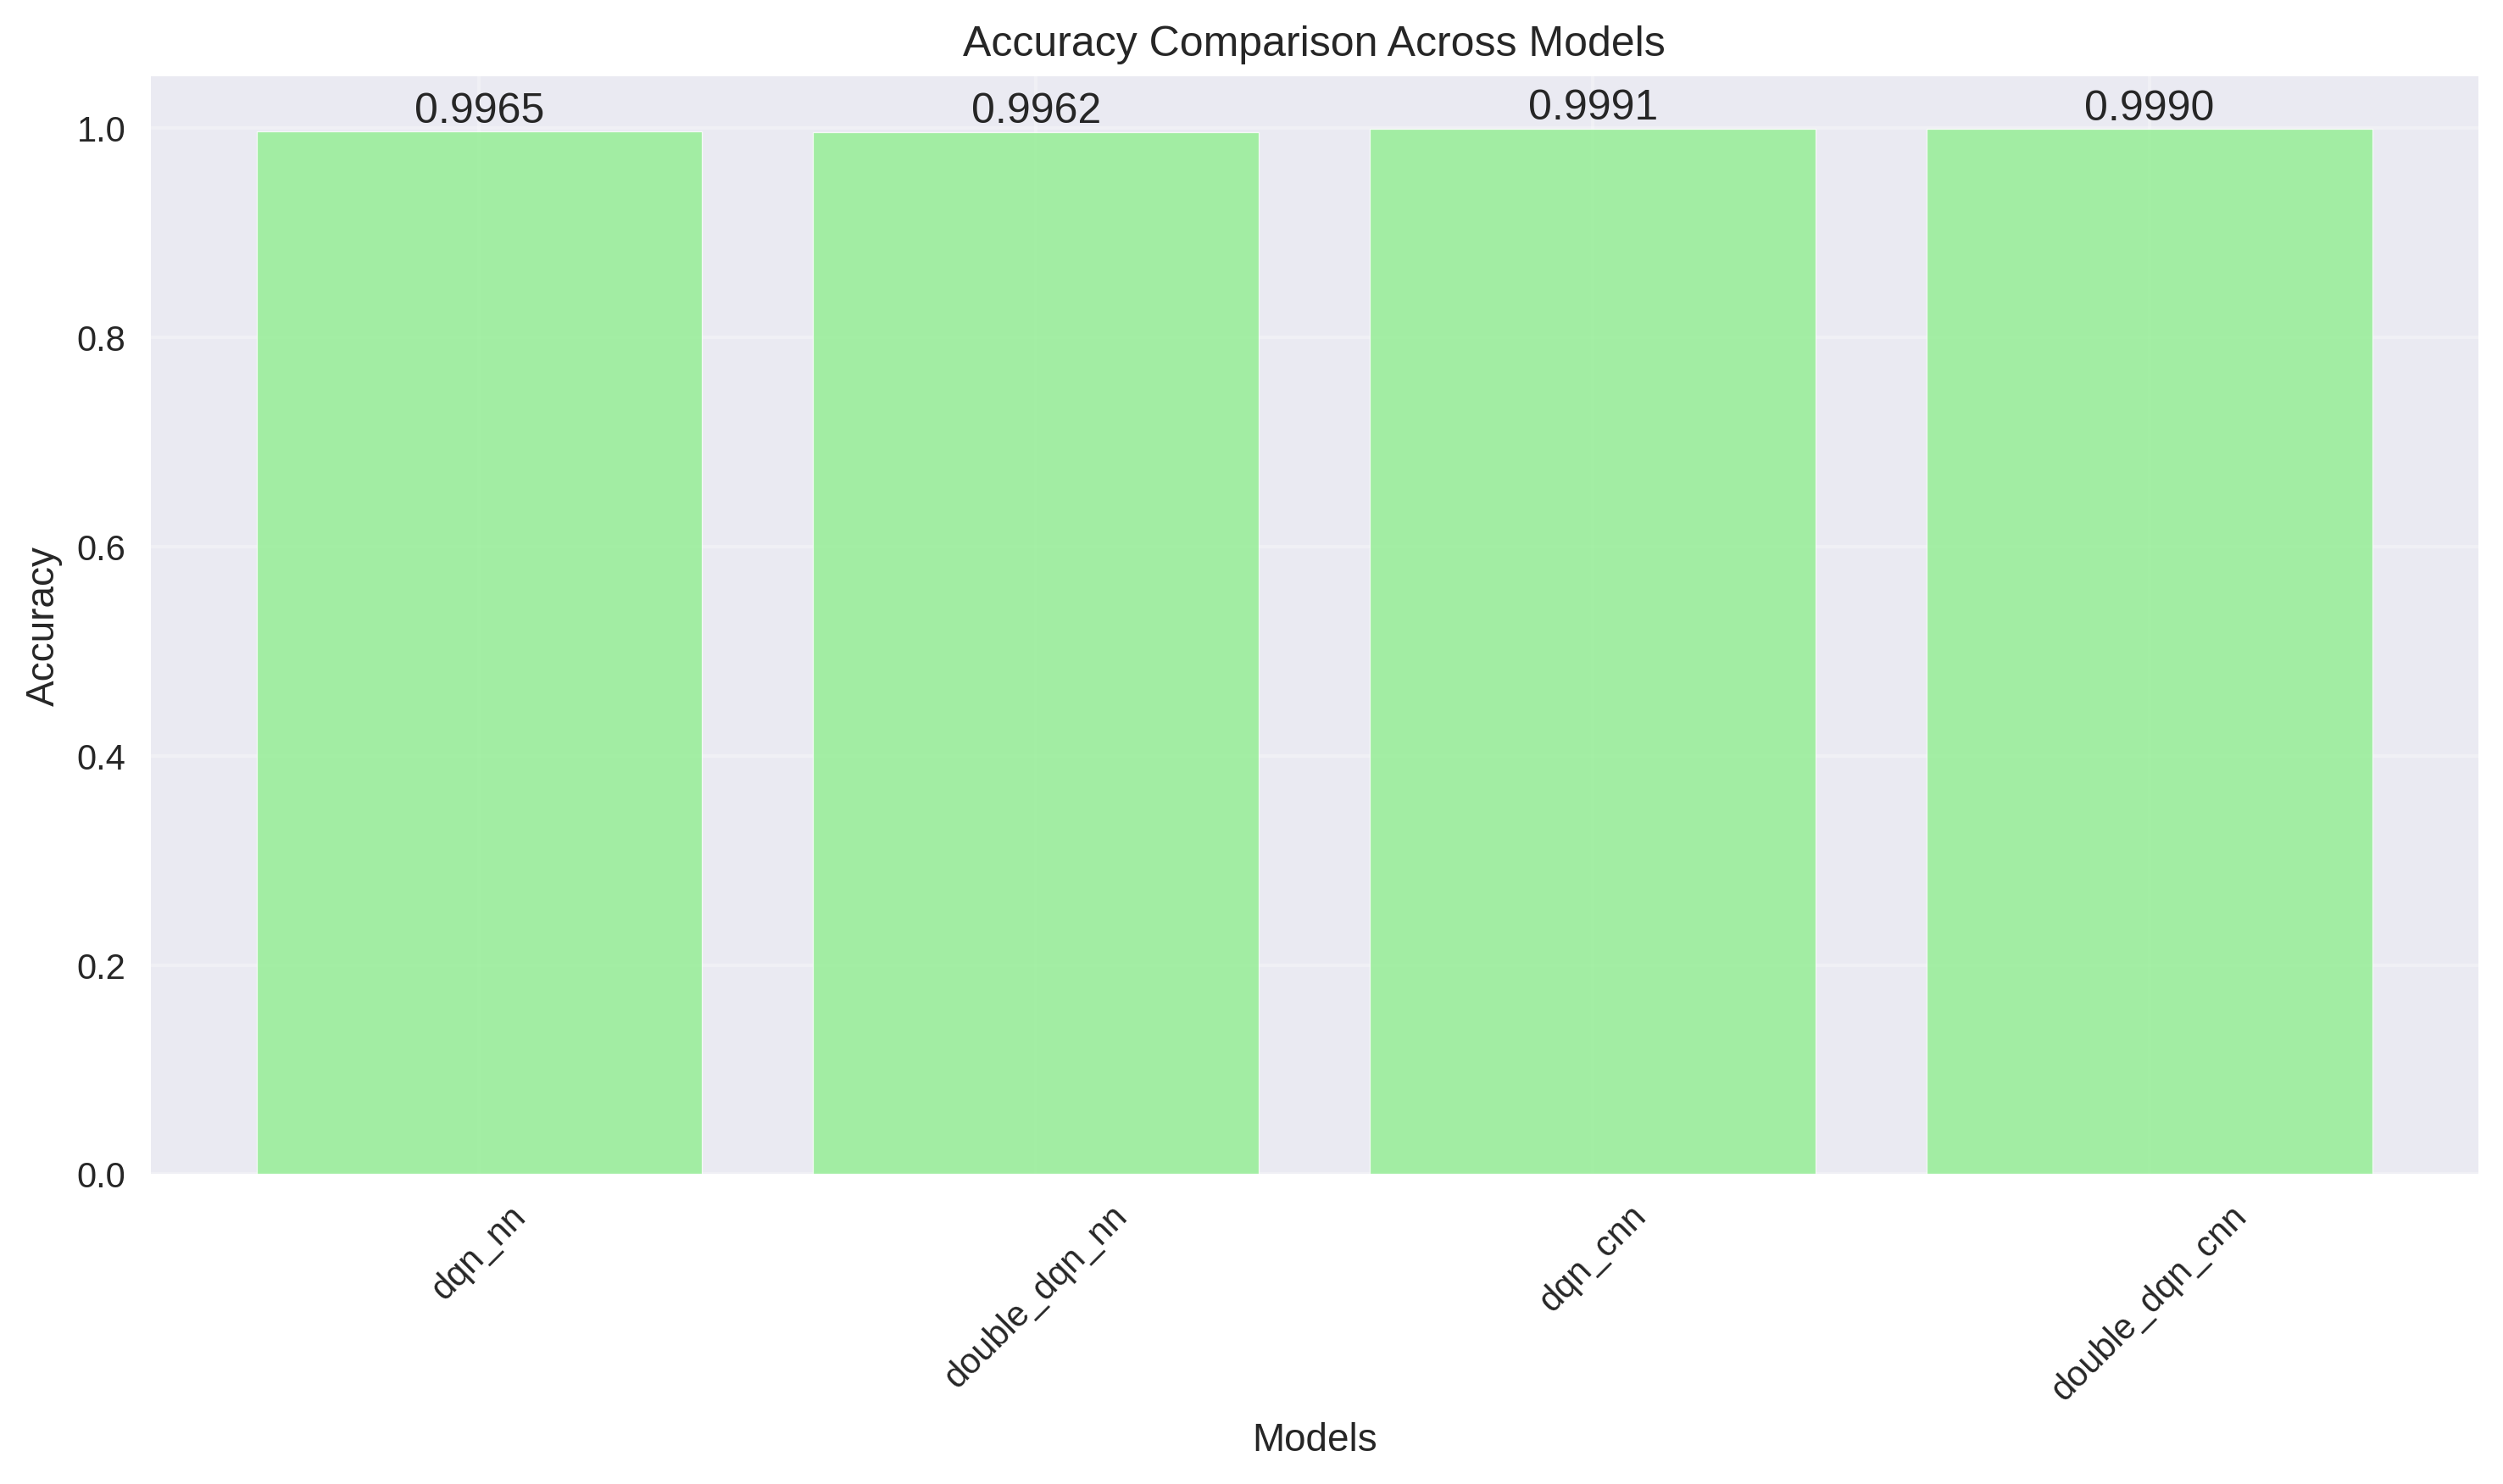
\includegraphics[width=0.8\textwidth]{images/accuracy_comparison.png} % Replace with your actual comparison bar chart
    \caption{Accuracy Comparison Across All Models and Tasks}
    \label{fig:accuracy_comparison}
\end{figure}
\begin{figure}[H]
    \centering
    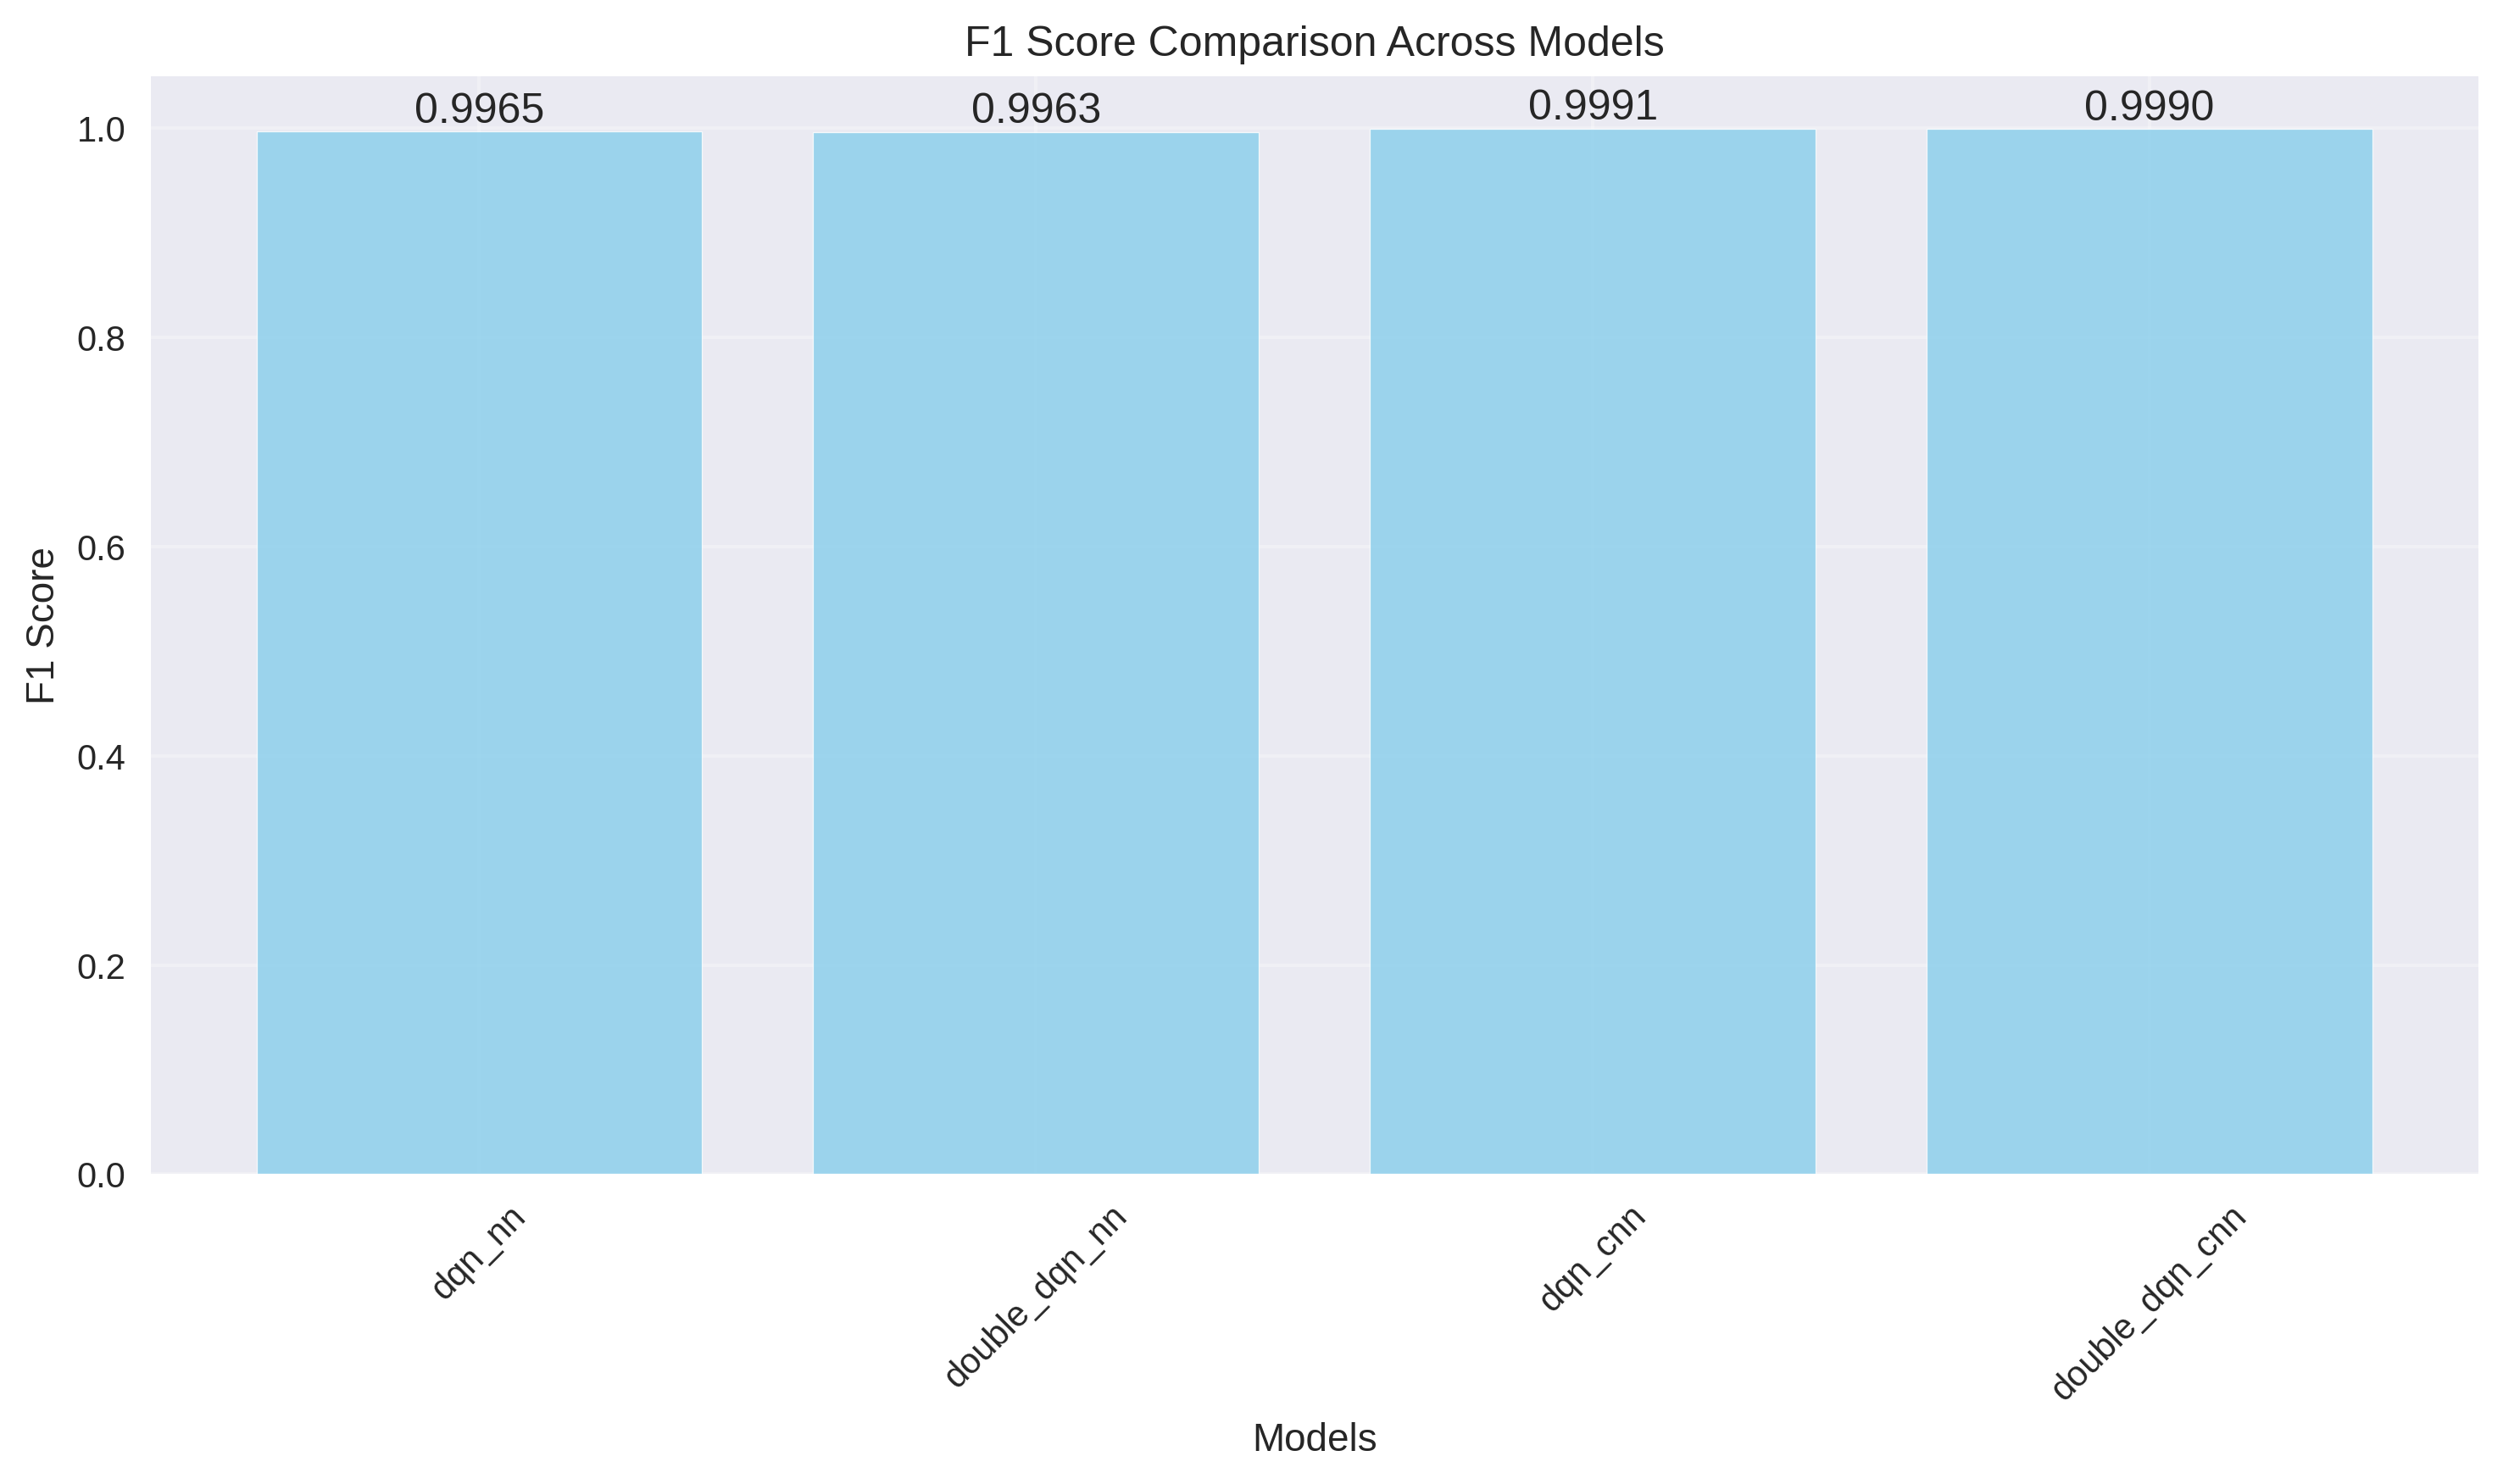
\includegraphics[width=0.8\textwidth]{images/f1_score_comparison.png} % Replace with your actual comparison bar chart
    \caption{F1-Score Comparison Across All Models and Tasks}
    \label{fig:f1_score_comparison}
\end{figure}
\begin{figure}[H]
    \centering
    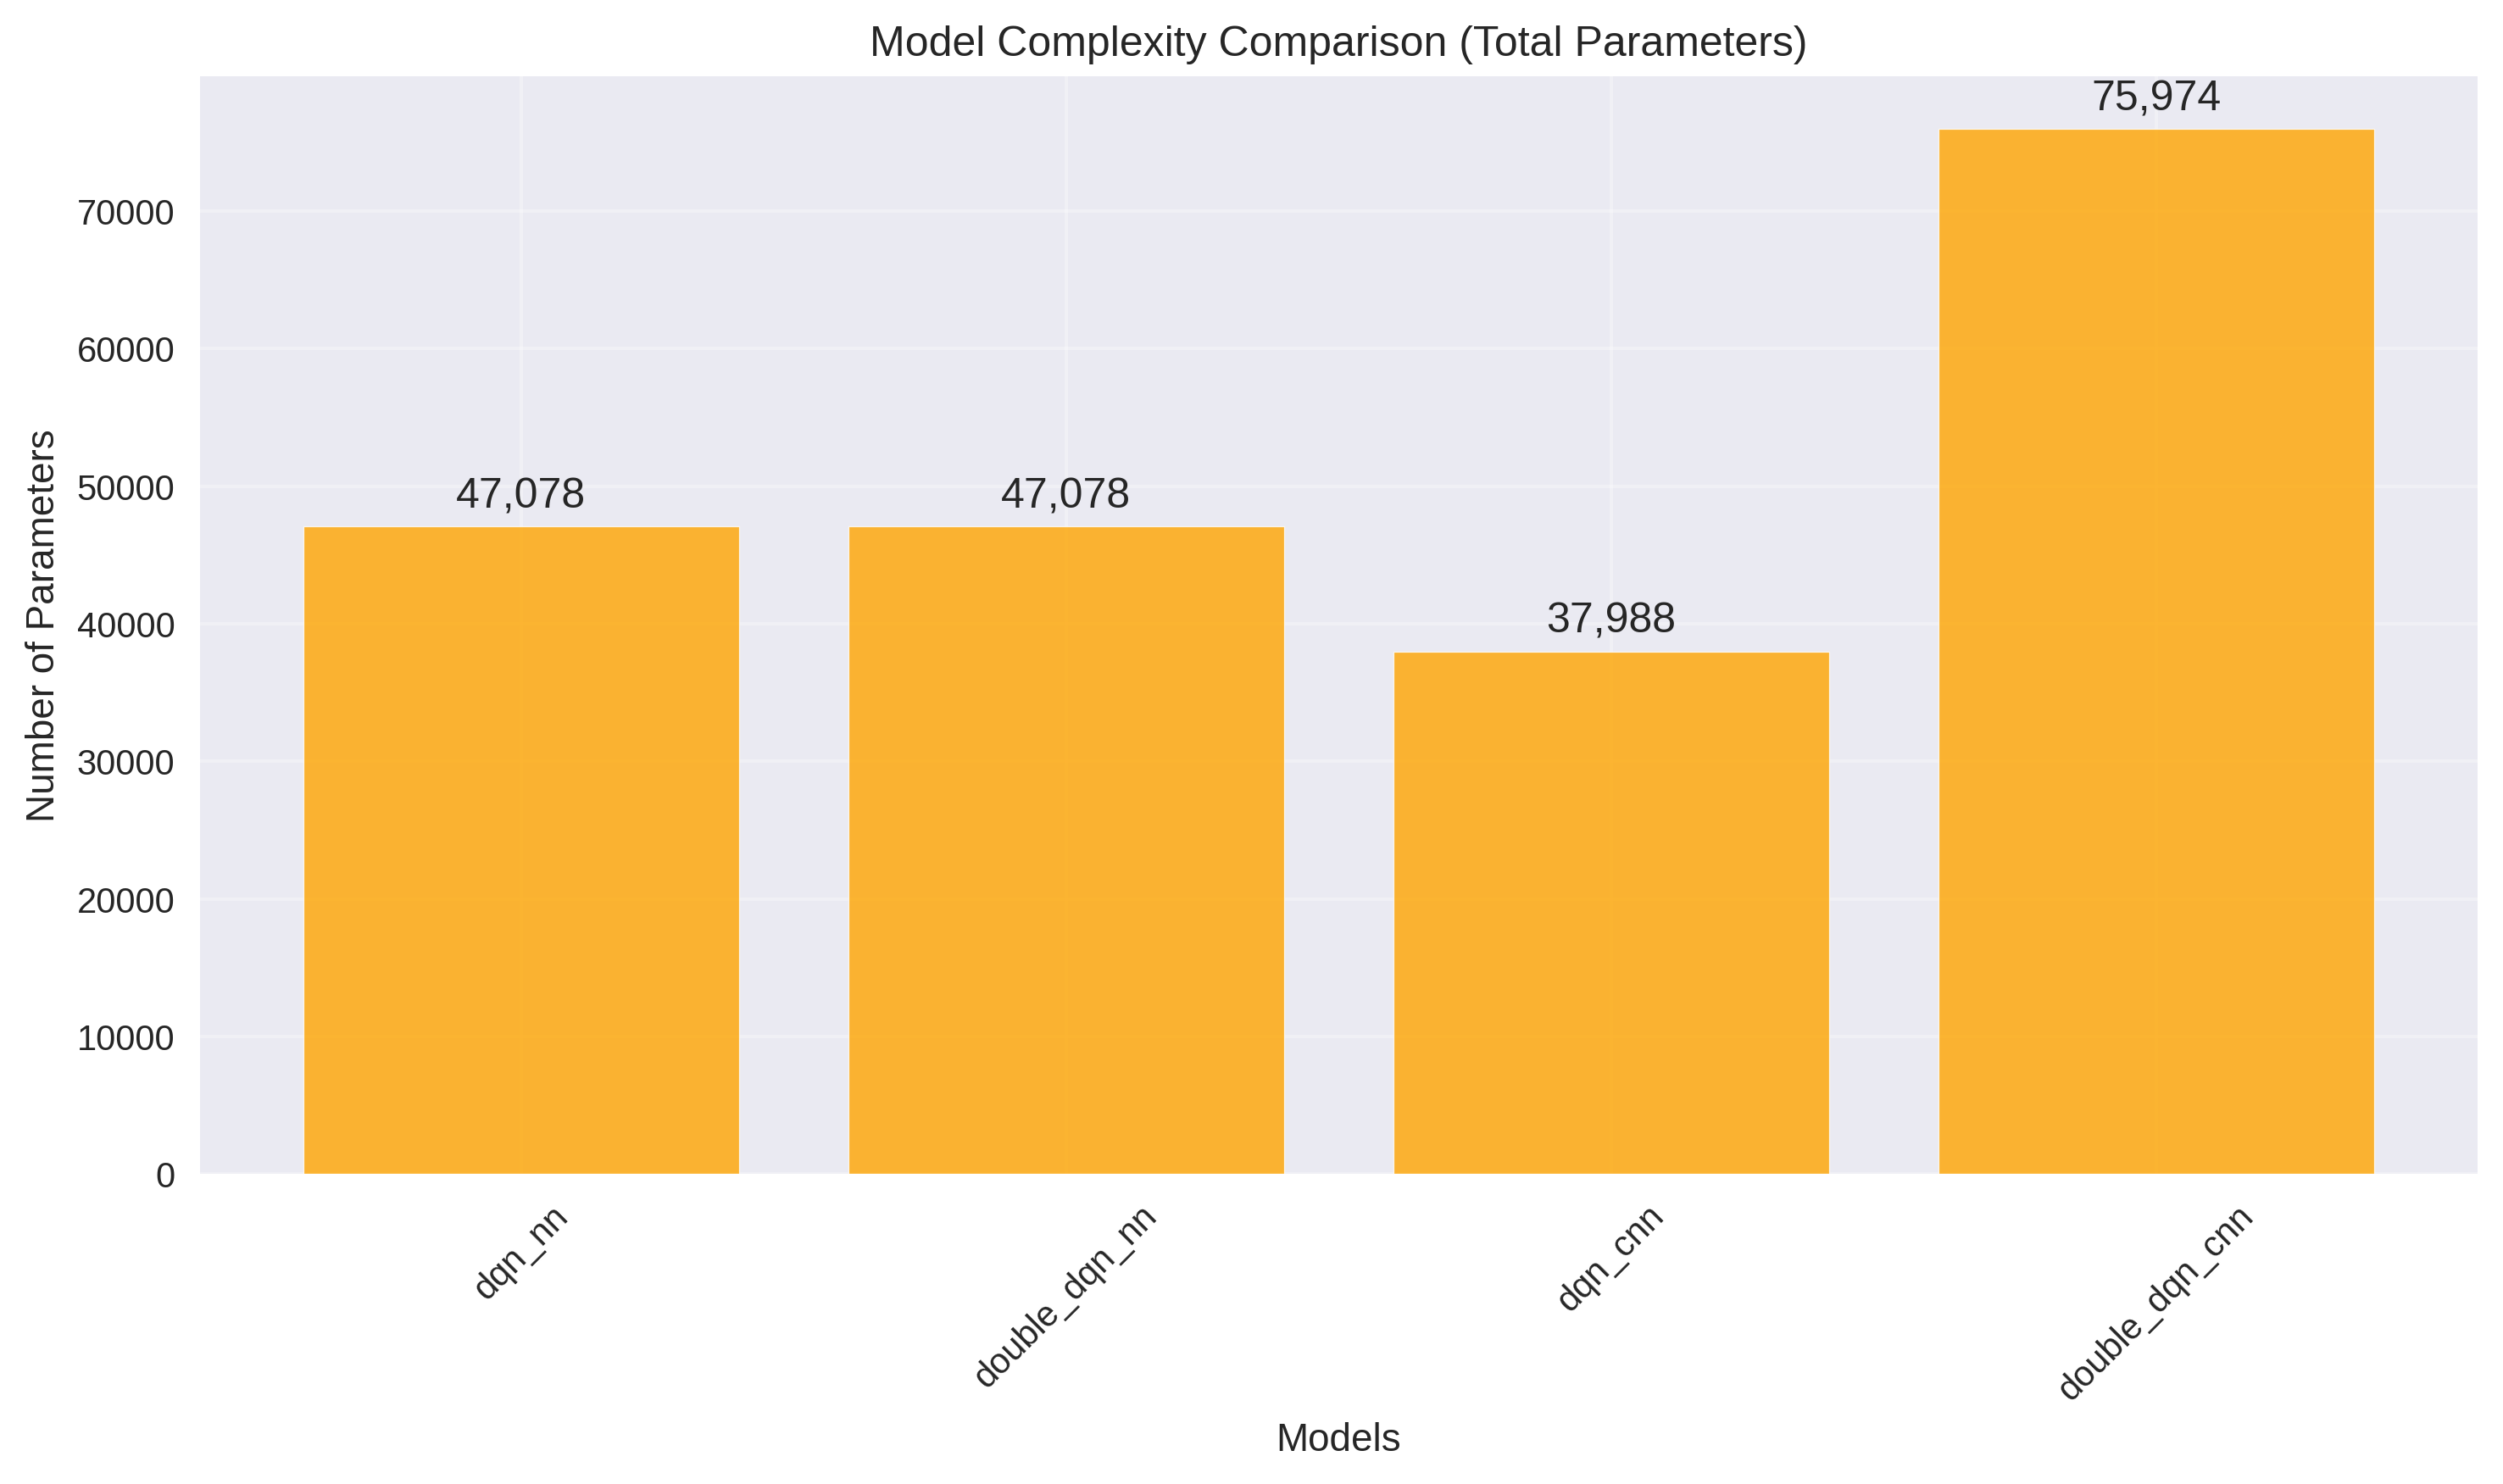
\includegraphics[width=0.8\textwidth]{images/model_complexity_comparison.png} % Replace with your actual comparison bar chart
    \caption{Model complexity Comparison Across All Models and Tasks}
    \label{fig:model_complexity_comparison}
\end{figure}
\begin{figure}[H]
    \centering
    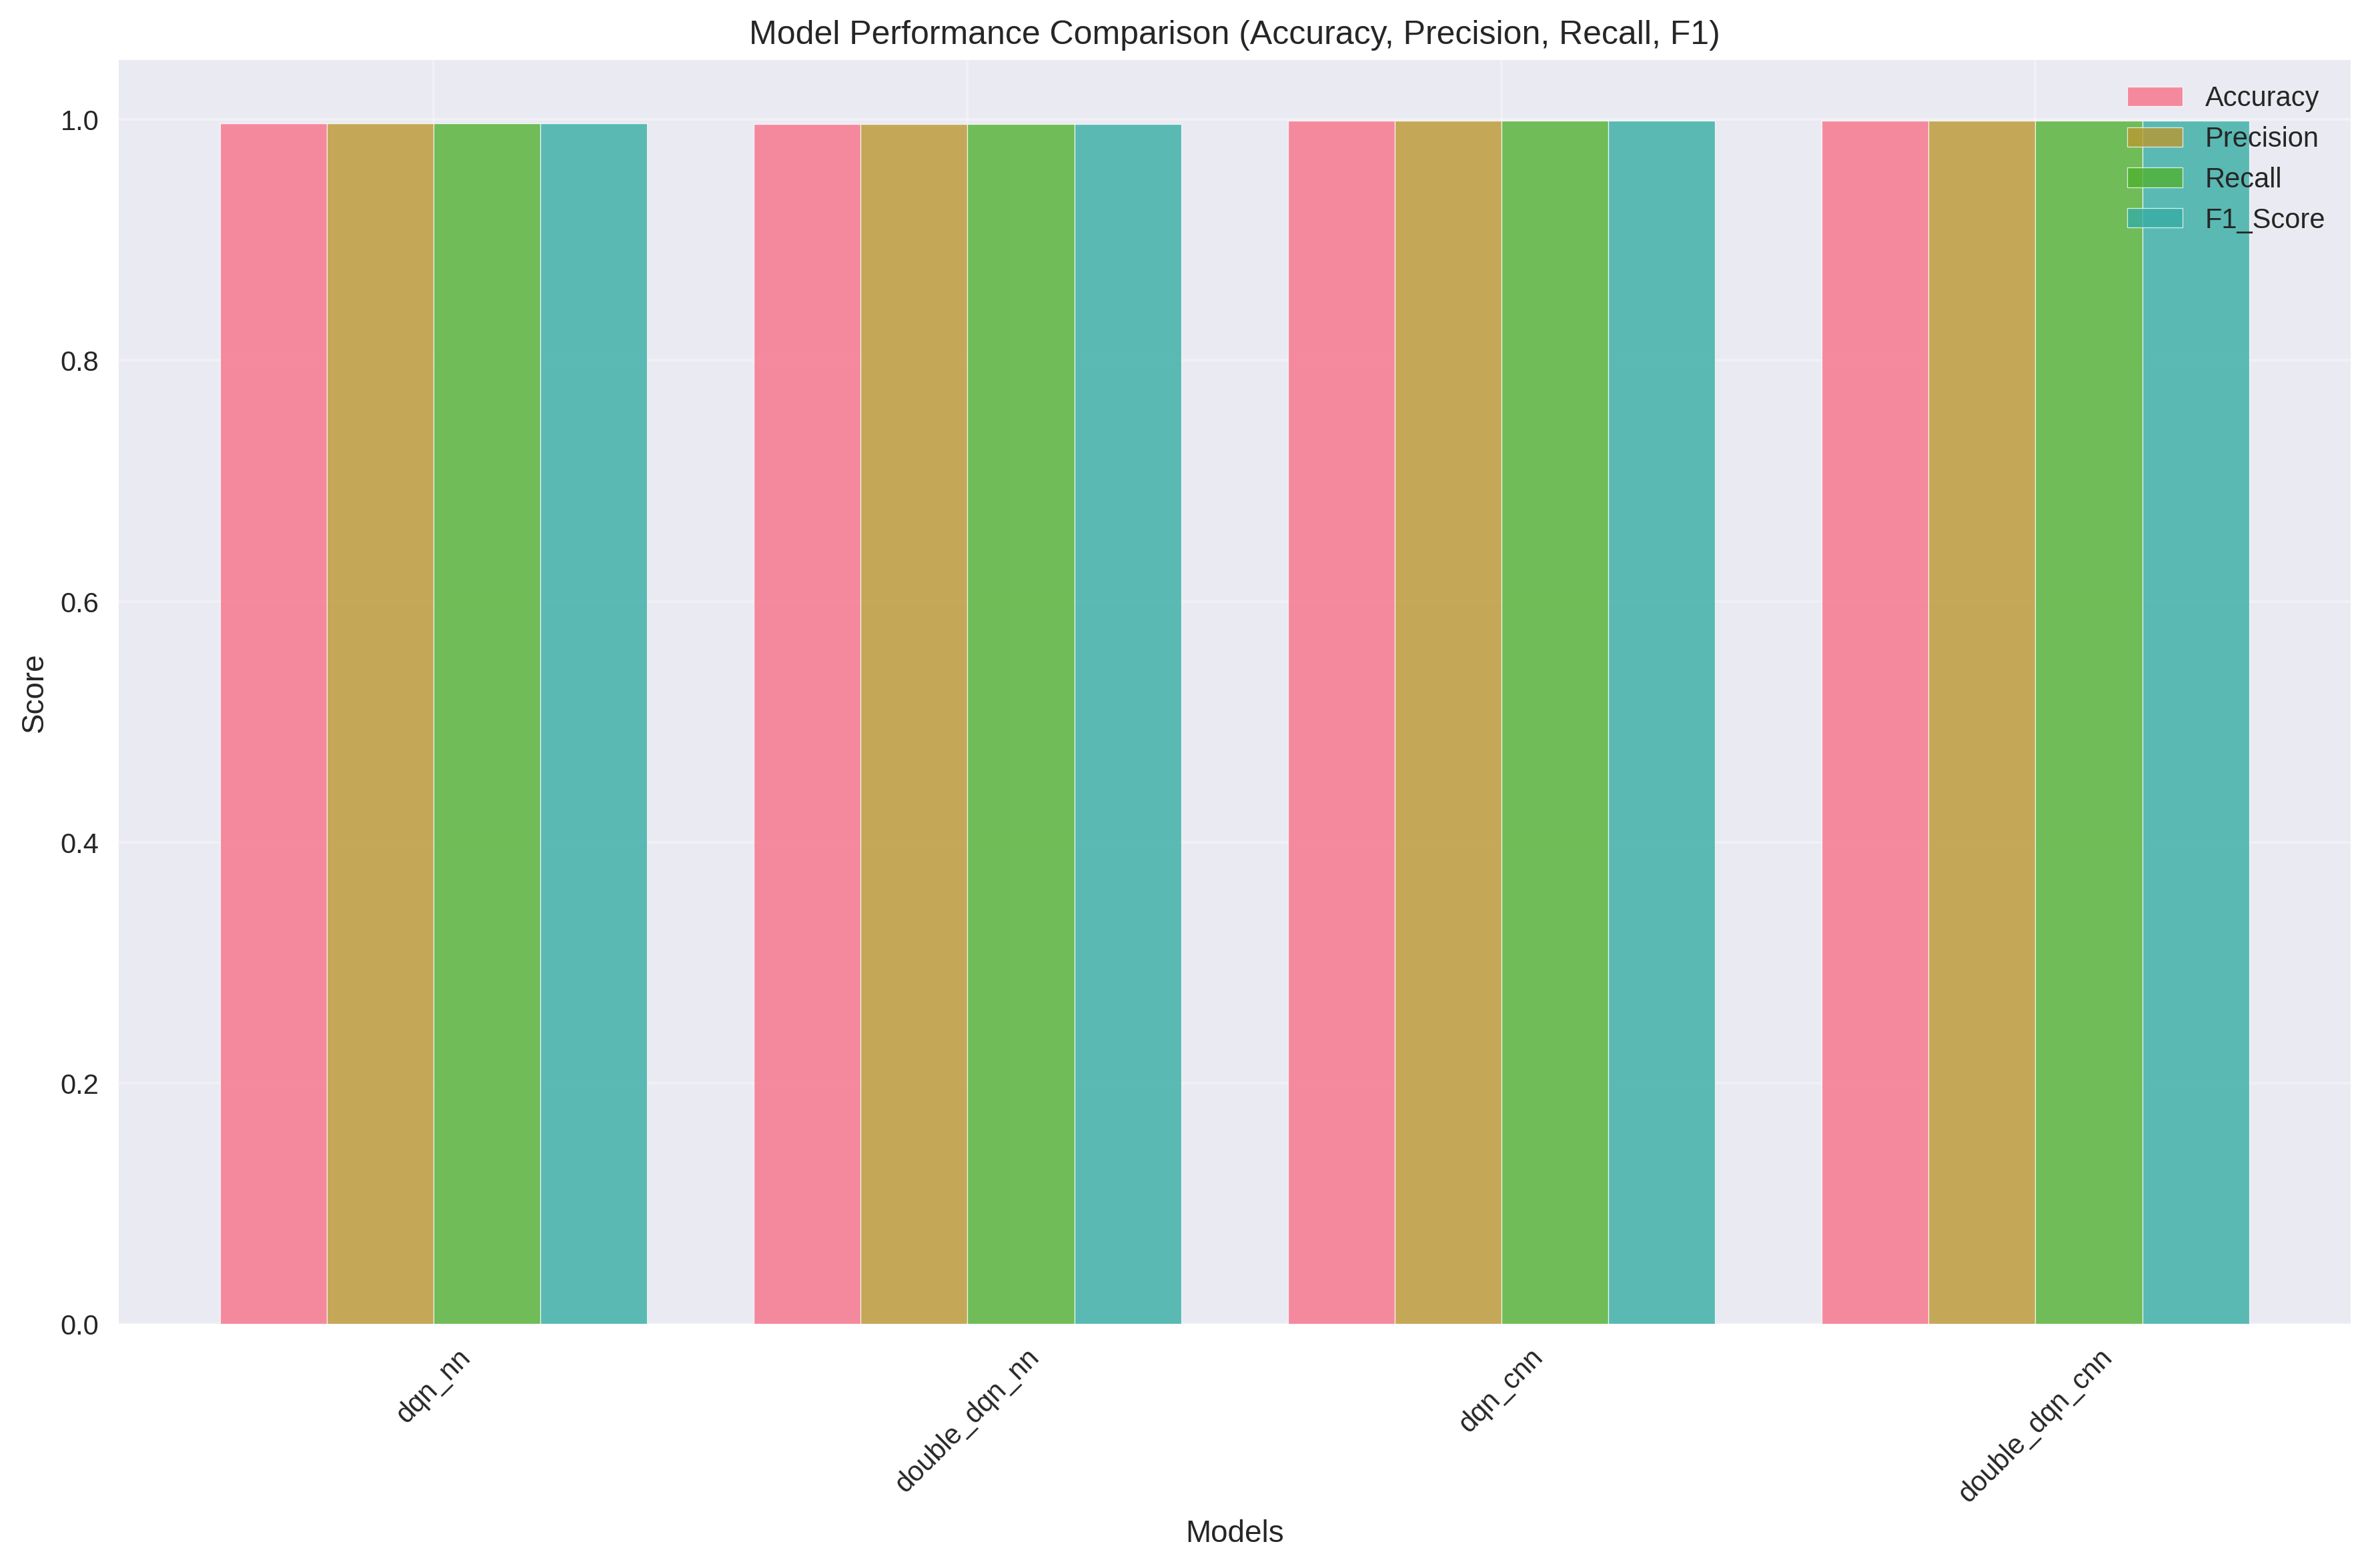
\includegraphics[width=0.8\textwidth]{images/performance_metrics_comparison.png} % Replace with your actual comparison bar chart
    \caption{Performance metrics Across All Models and Tasks}
    \label{fig:performance_metrics_comparison}
\end{figure}

Several key observations can be drawn from the results:
\begin{enumerate}
    \item \textbf{CNN-DQN Superiority:} Across both binary and multi-class tasks, the CNN-DQN model consistently delivered the highest performance. This validates our hypothesis that there are exploitable spatial correlations within the network features when arranged in an image-like format. The CNN's ability to learn hierarchical patterns provides a distinct advantage over the MLP, which treats features independently.
    \item \textbf{Effectiveness of DDQN:} The DDQN algorithm provided a modest but consistent performance boost over the standard DQN in both scenarios. This highlights the practical benefit of using DDQN to mitigate the Q-value overestimation problem, leading to more stable training and a more reliable policy.
    \item \textbf{Task Complexity Impact:} As expected, all models performed better on the binary classification task than on the multi-class task. The drop in performance for the multi-class scenario reflects the increased complexity of distinguishing between multiple subtle attack variations versus simply separating attack from benign traffic.
    \item \textbf{Viability of the RL Approach:} Most importantly, the extremely high scores achieved by all models, particularly the CNN-DQN (99.46% F1-Score in binary, 97.58% in multi-class), strongly demonstrate that adapting a DQN framework for a supervised classification task is not only feasible but also highly effective for DDoS detection.
\end{enumerate}

\section{Conclusion}
The experiments conducted in this chapter successfully evaluated the performance of our proposed RL-based detection models. The results clearly indicate that the CNN-DQN architecture is the most effective, achieving state-of-the-art detection rates on the CIC-DDoS2019 dataset for both binary and multi-class classification. The findings validate the novel approach of transforming tabular network data into a feature-image and leveraging a CNN for pattern extraction. Furthermore, the consistent, albeit smaller, gains from the DDQN algorithm underscore the importance of algorithmic stability in achieving robust performance. Overall, this empirical evaluation confirms that our DQN-powered system offers a powerful and accurate solution for modern DDoS detection.

\chapter*{General Conclusion}
\addcontentsline{toc}{chapter}{General Conclusion}

This thesis embarked on an exploration of a novel methodology for detecting Denial-of-Service (DoS) attacks by adapting the principles of Reinforcement Learning (RL), specifically Deep Q-Networks (DQN), to a traditionally supervised classification problem. Motivated by the limitations of static, signature-based Intrusion Detection Systems (IDS), which struggle against novel and evolving threats, our work sought to develop a more dynamic, adaptive, and intelligent detection framework. By reframing network traffic classification as a sequential decision-making process, we successfully designed, implemented, and evaluated a system capable of achieving exceptional detection accuracy.

\section*{Summary of Contributions}
The primary contributions of this research are multifaceted and can be summarized as follows:
\begin{enumerate}
    \item \textbf{A Novel Methodological Bridge:} We successfully developed a framework that bridges the gap between Reinforcement Learning and supervised classification for the cybersecurity domain. By simulating an RL environment from a static dataset and engineering a hybrid reward and target mechanism, we demonstrated how a DQN agent can be effectively trained to perform a classification task.
    \item \textbf{Advanced Architectural Design:} We proposed and implemented two distinct neural network architectures for the Q-function approximator: a standard Multi-Layer Perceptron (MLP) and a more advanced Convolutional Neural Network (CNN). The CNN-based approach, which involved a novel transformation of tabular feature vectors into 2D "feature-images," proved to be particularly innovative and effective.
    \item \textbf{Rigorous Empirical Validation:} The proposed models were rigorously trained and evaluated on the comprehensive and modern CIC-DDoS2019 dataset. Our top-performing model, the CNN-DQN, achieved an F1-Score of 99.46\% in binary classification and 97.58\% in multi-class classification, demonstrating state-of-the-art performance and confirming the viability of our approach.
    \item \textbf{Comparative Analysis:} Through a detailed comparison, we empirically proved the superiority of the CNN-based architecture for this task and quantified the stability improvements gained by using a Double DQN (DDQN) algorithm over the standard DQN.
\end{enumerate}

\section*{Study Limitations}
While the results are highly promising, it is important to acknowledge the limitations of this study, which also pave the way for future work:
\begin{itemize}
    \item \textbf{Static Environment:} The RL agent was trained and evaluated on a static, pre-collected dataset. This means the agent could not learn from the true, real-time consequences of its actions (e.g., how blocking traffic might alter an attacker's strategy). The full adaptive potential of RL is best realized in a live, dynamic environment.
    \item \textbf{Dataset Dependency:} The models' performance was validated on the CIC-DDoS2019 dataset. While comprehensive, its characteristics may not perfectly represent all real-world network environments. Generalization to different network architectures or entirely new zero-day attacks not represented in the training data remains an open question.
    \item \textbf{Feature Engineering Dependency:} The success of the CNN-DQN model is contingent on the effective construction of the feature-image. The ordering and grouping of features in this grid can impact performance, and the optimal arrangement may vary for different datasets.
    \item \textbf{Computational Overhead:} Training deep reinforcement learning models is computationally more intensive and time-consuming compared to traditional machine learning algorithms like Decision Trees or SVMs, which could be a consideration for resource-constrained environments.
\end{itemize}

\section*{Future Research Directions}
This research opens up several exciting avenues for future investigation:
\begin{itemize}
    \item \textbf{Online and Interactive Learning:} The most critical next step is to deploy the RL agent in a live or highly realistic simulated network environment. This would enable online learning, where the agent can continuously adapt its policies based on real-time feedback and the evolving nature of network traffic.
    \item \textbf{Exploration of Advanced RL Algorithms:} This work focused on DQN and DDQN. Future research could explore more advanced, state-of-the-art RL algorithms, such as Proximal Policy Optimization (PPO) or Asynchronous Advantage Actor-Critic (A3C), which may offer improved sample efficiency and stability.
    \item \textbf{Integration of Explainable AI (XAI):} A significant challenge with deep learning models is their "black box" nature. Integrating XAI techniques like SHAP (SHapley Additive exPlanations) or LIME (Local Interpretable Model-agnostic Explanations) could provide insights into *why* the agent classifies a certain flow as malicious, increasing trust and interpretability for security analysts.
    \item \textbf{Hierarchical and Multi-Agent RL:} A complex network could be defended by a team of RL agents. A hierarchical system could have a high-level agent that identifies a potential threat and delegates the detailed classification to specialized agents trained on specific attack families (e.g., one for volumetric attacks, another for protocol attacks).
    \item \textbf{Automated Reward Shaping and Feature Learning:} Future work could investigate methods for automatically learning the reward function or using techniques like autoencoders to learn the most effective feature representations, reducing the reliance on manual feature engineering.
\end{itemize}

In conclusion, this thesis has successfully demonstrated that Reinforcement Learning provides a powerful and promising paradigm for building the next generation of intelligent and adaptive Intrusion Detection Systems. By learning to make optimal decisions in the face of uncertainty, RL-powered agents are well-positioned to defend against the dynamic and ever-evolving landscape of cyber threats.


\begin{thebibliography}{99}

\bibitem{ibm_security_fundamental}
IBM, \emph{Security Fundamentals},\\
\url{https://www.linkedin.com/pulse/fundamentals-security-slammghana/}

\bibitem{ibm_principles_of_information_security}
CIA, \emph{Principles of Information Security},\\
\url{https://www.cleanpng.com/png-information-security-confidentiality-availability-1373941/}

\bibitem{fidelis_dos}
Fidelis Security, \emph{Understanding DoS and DDoS Attacks},\\
\url{https://fidelissecurity.com/blog/dos-ddos-attacks}

\bibitem{imperva_dos}
Imperva, \emph{Denial of Service (DoS) Attack},\\
\url{https://www.imperva.com/learn/ddos/denial-of-service/}

\bibitem{netscout_slowloris}
NETSCOUT, \emph{Slowloris Attack},\\
\url{https://www.netscout.com/blog/asert/slowloris-attack}

\bibitem{mdpi_dos}
MDPI, \emph{Anomaly-based Detection of DDoS Attacks Using Machine Learning},\\
\url{https://www.mdpi.com/2076-3417/10/3/1052}

\bibitem{ibm_ids}
IBM, \emph{What is an Intrusion Detection System (IDS)?},\\
\url{https://www.ibm.com/think/topics/intrusion-detection-system}

\bibitem{wikipedia_ids}
Wikipedia, \emph{Intrusion Detection System},\\
\url{https://en.wikipedia.org/wiki/Intrusion_detection_system}

\bibitem{fortinet_ids}
Fortinet, \emph{What is Intrusion Detection Systems (IDS)? How does it Work?},\\
\url{https://www.fortinet.com/resources/cyberglossary/intrusion-detection-system}

\bibitem{techtarget_ids}
TechTarget, \emph{What Is an Intrusion Detection System (IDS)?},\\
\url{https://www.techtarget.com/searchsecurity/definition/intrusion-detection-system}

\bibitem{cicddos2019}
Canadian Institute for Cybersecurity, \emph{CIC-DDoS2019 Dataset},\\
\url{https://www.unb.ca/cic/datasets/ddos-2019.html}

\end{thebibliography}



\end{document}

